\documentclass[11pt]{article}

\usepackage[margin=1in]{geometry}
\usepackage{amsmath,amssymb,amsthm}
\usepackage{booktabs}
\usepackage{graphicx}
\usepackage{xcolor}
\usepackage[round]{natbib}
\usepackage[colorlinks=true,linkcolor=blue,citecolor=blue,urlcolor=blue]{hyperref}

\bibliographystyle{plainnat}

\emergencystretch=3em

\newtheorem{proposition}{Proposition}
\newtheorem{corollary}{Corollary}
\theoremstyle{remark}
\newtheorem{remark}{Remark}

\title{An Omitted Mode Is a Rare Rule: The Sampling-Verification Danger Law in Continuous Code World Models}

\author{Javier Aguilar Mart\'in\\ AGILabs (\href{https://javieraguilar.ai}{javieraguilar.ai})}

\date{}

\begin{document}

\maketitle

\begin{abstract}
In the Code World Model (CWM) paradigm an LLM synthesizes an executable world model that a classical planner searches, accepted when it matches sampled transitions. In discrete games, a companion paper showed this gate certifies the wrong thing: a model can pass at 100\% transition accuracy and still lose, following $\mathrm{danger} = \mathrm{play\_cost} \times (1-\mathrm{rarity})^N$ \citep{aguilar2026verified}. This paper moves to continuous state spaces, where model-based RL treats world-model error as \emph{pervasive}, not localized. The law transfers (its ingredients are measure-theoretic) and we prove smooth (Lipschitz) pairs cannot realize the \emph{exactly} localized verified-but-wrong geometry (Section~\ref{sec:theory}): exact localization requires unbounded local Lipschitz structure, which hybrid boundaries supply, so an omitted mode is a rare rule. On two 1D hybrid instruments the gate misses the mode at the predicted $(1-r)^N$ rate and the mode-blind planner is exploited below random at every knob once the phantom reward's tail is removed, play\_cost knob-invariant to ${\approx}1.5\times10^{-4}$; a distrust-region planner collapses this to a single-contact transient, which we show is a separation fact rather than a covering one. With real LLM synthesis, on 1D every sample missing the mode yielded a certified, blind, exploited model; when it contained the mode, GPT-5.x repaired the exact rule (109/111) --- unlike the discrete setting. But repair is geometry-dependent: on a 4D bi-modal instrument with 2D modes it inverts. Neither GPT-5.x size recovers the region rule in any of \textbf{156} mode-containing seeds (disc, zero-curvature square, $3\times$-budget guidance); a Claude arm fails the same way. The mechanism the evidence is consistent with is a \emph{template prior} over low-complexity regions (half-planes on the disc, discs on the square), not boundary curvature, so the law's exhaustiveness is geometry-scoped; certification stays sound. Identifiability is a sample property; repair is model- and geometry-dependent. Localization --- both the danger and the repair --- is a representational property of \emph{code}.
\end{abstract}

\section{Introduction}
\label{sec:intro}

The companion paper \citep{aguilar2026verified} established, in discrete games, that transition accuracy on randomly sampled play-throughs is the wrong adequacy criterion for a world model used in planning, and quantified the failure: $\mathrm{danger} = \mathrm{play\_cost} \times (1-\mathrm{rarity})^N$, with the gate-miss factor exact under i.i.d.\ sampling. Its related-work discussion closed with a promissory note: the rare-rule gap is a localized, discrete failure that state-accuracy metrics mask by dilution --- a point worth revisiting in continuous settings, where the model-based RL literature \citep{lambert2020objective,hafner2020dreamer,janner2019mbpo} treats world-model error as pervasive and compounding rather than localized and pivotal.

This paper is that revisit. The question is not whether continuous world models can be wrong --- that literature is mature --- but whether the specific \emph{verified-but-wrong} geometry of the discrete result exists in continuous state spaces: a model that passes a sampling gate cleanly, is (in a precise sense) almost-everywhere correct, and is still exploited catastrophically by the planner that trusts it.

The answer is yes, and the continuous version of the story is in one respect cleaner than the discrete one. The discrete headline had two components: (a) a provable one (when the rare rule is absent from the sample, no learner can infer it \emph{from the sample} --- an identifiability event with probability exactly $(1-r)^N$) and (b) an empirical one (the LLMs tested did not infer the rule \emph{even when it was present} --- ``translation, not inference''). In the continuous \emph{one-dimensional} instruments the second component \textbf{vanishes for one of the three families we measured}: GPT-5.x infers an omitted hybrid mode from a handful of boundary-crossing transitions, writing the exact global rule. This turns out to be \emph{geometry-dependent}: on a third instrument, a 4D bi-modal patch field whose modes are 2D regions rather than 1D clamps, the residual returns --- neither GPT-5.x size recovers the region rule from data (0/156 mode-containing attempts over 20 distinct gate samples pooled over the disc, a zero-curvature square ablation, and a strongest-effort prompting/budget treatment), and a Claude cross-family arm on the same cell reproduces the same failure classes (Section~\ref{sec:patch2d-synthesis}), so ``translation, not inference'' comes back on two-dimensional boundaries even for the model that erased it on the clamps. Of the discrete headline's two components, what remains provable is exactly the gate-miss and identifiability propositions (Section~\ref{sec:theory}): with the mode absent from the sample --- the $(1-r)^N$ event --- no learner can recover it from the sample alone (a prior or the specification could still supply it; Proposition~\ref{prop:ident}). Sample-covered exactness is the acceptance criterion itself; that every accepted artifact's \emph{off-sample} content was also the true mode --- with a single exception, a prior-injected phantom mode erring only where its sample is silent --- is an empirical, code-inspected regularity for the models tested (GPT-5.x repairs every revealed clamp; Qwen stalls and the gate refuses its patches; Claude repairs most through a symmetry prior), not a theorem. The danger law here is not just exact; empirically, for the models tested, it is exhaustive \emph{on the 1D instruments} --- and Section~\ref{sec:patch2d-synthesis} shows that this exhaustiveness is itself geometry-scoped, failing on a 2D circular mode.

Contributions:
\begin{enumerate}
\item \textbf{Theory: three propositions transfer, ten are new.} The companion paper's gate-miss, identifiability and play-cost propositions transfer with only notational change, being measure-theoretic (Section~\ref{sec:theory}). Its genuinely discrete ingredient is the \emph{localization premise}, and we prove it requires unbounded local Lipschitz structure: for $L$-Lipschitz truth and model differing by $\eta$ at a point, the disagreement region contains a metric ball of radius $(\eta-\varepsilon)/2L$ (Proposition~\ref{prop:lipschitz}), so hybrid mode boundaries are exactly where the obstruction disappears and an omitted mode is a rare rule. Beyond those two the continuous setting forces, and rewards, the rest: a \emph{sharp} distribution-free bracket for the multi-mode joint gate-miss factor, replacing an independence assumption with none (Proposition~\ref{prop:jointmiss}); an identity showing the reveal-rarity's $\varepsilon$-invariance is exact below a threshold, together with the proof that no such threshold survives in the population and a quadratic rate that does (Propositions~\ref{prop:epsinv} and~\ref{prop:epsrate}); \emph{derived} rather than estimated normalizers for the play-cost ceiling, which removes the last measured supremum from Corollary~\ref{cor:playcost} (Proposition~\ref{prop:normalizers}); a coverage certificate for Lipschitz pairs, and a partition form of it that is exact on this instrument and twice as strong (Propositions~\ref{prop:coverage} and~\ref{prop:partition}); a detectability rate making smoothness quantitative (Proposition~\ref{prop:detectrate}); and a packing bound on the mitigation's fencing cost (Proposition~\ref{prop:fencecover}).

  We are explicit throughout about which side of the line each claim sits on. Proved: everything just listed, each with its hypotheses stated and its instantiating constants derived by scripts the numeric audit reads. Measured, and labelled as such: the LLM repair and non-repair counts, the $2$D lock-in rate, the CEM regime, the rarity values themselves, and --- after an honest attempt that got only part of the way --- how the exploited planner's pinning \emph{starts}.
\item \textbf{Two minimal hybrid instruments and two planner families} --- cart-with-wall (linear off-mode plant) and pendulum-with-stop (nonlinear) --- on which the full discrete phenomenology is measured with the same harness and planner, and no per-instrument re-calibration of either (the reward widths and fence bands do differ per instrument): the threshold law with the whole $(1-r)^N$ elbow inside the knob sweep, knob-invariant $\mathrm{play\_cost} \approx 1$ under random-shooting model-predictive control (MPC), and the reach mechanism in its cleanest form (Section~\ref{sec:mechanism}). A fixed cross-entropy-method (CEM) planner has near-zero play cost on all 11 rows with strictly lower imagined mode-crossing than MPC; on the two rows where its crossing fraction is exactly zero this is the bound's other branch, and on the other nine the bound is vacuous and the result is empirical (Section~\ref{sec:cem}). Three instrument-design lessons of independent value are recorded (Section~\ref{sec:lessons}).
\item \textbf{A pinned-integrator contract and a measured axis separation.} The pinned-integrator synthesis contract makes correct code float-exact --- a property of code exactness independent of the gate's tolerance --- so the synthesis gate (Section~\ref{sec:synthesis}) can run at $\varepsilon = 10^{-9}$. Separately, at a deployment-realistic $\varepsilon = 0.01$ (Section~\ref{sec:axes}), the gate rejects supra-tolerance global bias on every rollout, passes sub-tolerance bias harmlessly, and misses the hard mode at a rate that closely tracks the predicted $(1-r)^N$ (within sampling noise at gate scale; Section~\ref{sec:axes}). A smooth localized perturbation of comparable rarity has $\approx 0$, at higher amplitude \emph{negative}, play cost.
\item \textbf{A measured planner-side mitigation} (Section~\ref{sec:mitigation}): distrust-region replanning --- the planner checks its model's predictions against observed transitions and fences the refuted predictions --- collapses the pinned-forever exploitation (below random at 7 of those 11 rows; Section~\ref{sec:mechanism}) to a single-contact transient on all 11 knob rows across both hand-written \emph{1D} instruments, at zero cost when the model is right (bit-identical to plain MPC, tested). Why one contact suffices there is a separation fact rather than a covering one, and it is measured: the outcome is bit-identical over a $20\times$ range of the fence band. On a 2D circular mode the same fence degrades and, at the farthest knob, fails outright in $7$ of $20$ episodes, because its tie-break is an unsigned distance (Section~\ref{sec:patch2d-mitigation}). The gate-side law is untouched throughout: the gate still certifies a wrong model.
\item \textbf{The synthesis result: danger collapses to pure identifiability} (Section~\ref{sec:synthesis}). Real-LLM arms (GPT-5.x, 20 seeds/cell) with the identifiability event logged per seed: mode absent $\Rightarrow$ 20/20 verified-blind-exploited (regret 0.999; Wilson lower bound 0.84 over two \emph{disjoint} sample blocks, Section~\ref{sec:synthesis}); mode present $\Rightarrow$ repaired to the exact global rule (both sizes 10/10, large in $\le 1$ iteration), no artifact wrong on a transition its own sample covered was ever accepted in the GPT-5.x arms. Cross-family spot-checks in two more families reproduce the blind-exploited event in every family but diverge on repair --- Qwen repairs none (superstitious patches the gate refuses), Claude (agent-relayed) repairs most through a symmetry prior that can certify an invented mode unfalsifiable by its gate sample --- so repair-from-data is model-dependent in mechanism, while identifiability is a property of the sample, not the model. The whole result replicates on a second, nonlinear instrument (a pendulum with an angular hard stop): GPT-5.x repairs 62/62 mode-present seeds and every mode-absent seed is blind and exploited. On a third, 4D bi-modal instrument (PatchField2D) the repair finding \emph{inverts}: neither GPT-5.x size recovers the circular mode from data (0/76 mode-containing seeds), most often reducing the disc to a half-plane ($38/76$), and a Claude cross-family arm fails the same way. Two ablations then pin the mechanism: a \emph{zero-curvature square} is not repaired either (0/40 --- with the inverse error, discs written on square evidence), and region-first guidance at $3\times$ budget eliminates the half-plane yet yields hull fits of the one-sided contact evidence (0/40) --- \textbf{0/156 pooled}. Repair-from-data is geometry-dependent via a \emph{template prior} over region forms, not curvature, and the law's empirical exhaustiveness is correspondingly scoped --- while the all-or-nothing gate stays sound, certifying no partial artifact (Section~\ref{sec:patch2d-synthesis}).
\item \textbf{Smooth learners cannot localize} (Section~\ref{sec:smooth}): a closed-form linear fit on mode-free data passes both gates fully blind (identifiability is learner-independent); on mode-containing data it is tilted twelve orders of magnitude off-mode by four contact rows in 3200 while still missing the mode. Both the danger geometry and the repair capability are representational properties of code.
\end{enumerate}

Scope up front: three instruments (two 1D --- cart, pendulum --- plus a 4D bi-modal PatchField2D), two base planner families (random-shooting MPC and CEM, one fixed configuration each), 20 seeds per headline synthesis cell across the instruments (both GPT-5.x sizes; plus the caught cell on the pendulum and two bi-knob cells on PatchField2D), a 3-seed cross-family spot-check per 1D instrument (not full sweeps), and a probe-grade multilayer perceptron (MLP). Section~\ref{sec:limitations} gives the honest assessment and the full seed accounting.

\section{The instruments}
\label{sec:instrument}

This section specifies the hand-written hybrid instruments and the planner the later experiments reuse unless they say otherwise, and records the design lessons learned while calibrating them.

\subsection{Cart-with-wall}
\label{sec:cartwall}

State $(x, v)$; action $a \in [-a_{\max}, a_{\max}]$; semi-implicit Euler with fixed $dt$:
\[
a \leftarrow \mathrm{clamp}(a), \qquad
v' = v + (\mathrm{gain}\cdot a - \mathrm{drag}\cdot v)\,dt, \qquad
x' = x + v'\,dt,
\]
with defaults $dt = 0.1$, $\mathrm{gain} = 3$, $\mathrm{drag} = 0.3$, $a_{\max} = 1$. The \textbf{hybrid mode} is an inelastic wall at $x_\mathrm{wall}$: if $x' \geq x_\mathrm{wall}$, the next state is exactly $(x_\mathrm{wall}, 0)$. The \textbf{blind model} is the same code path with the wall branch removed --- the hand-written on-manifold proxy for a CWM synthesized from a spec that omits the wall, \emph{bit-exact off-mode by construction} (tested: exact float equality on wall-free trajectories). We call such a model \textbf{mode-blind} (the canonical term; instrument-specific synonyms like ``wall-blind'', or ``blind'' for short, mean the same thing). Reward is two sigmoid plateaus: a small reachable one on the left ($0.3$, at $x \leq -6$) and a large one on the right ($1.0$, at $x \geq 12$) whose approach every swept wall position blocks. Episodes are 80 steps from $x_0 \sim U(-0.5, 0.5)$, $v_0 = 0$.

The design requirements mirror the companion paper's material-at-cap instrument (paper 1's discrete instrument: a rare resource-cap rule likewise omittable from sampled play): (a) random rollouts rarely fire the mode --- the wall position is the \textbf{rarity knob} ($r$ sweeps $0.317 \to 0.0024$ over $x_\mathrm{wall} \in [2, 10]$; Table~\ref{tab:danger}); (b) the omission is \emph{exploited}, not merely mispredicted --- the wall-blind model predicts coasting through the wall toward the large plateau, so the planner it advises drives right and is pinned; (c) the truth planner's optimal play differs qualitatively --- it goes left.

The second instrument (pendulum with a hard angular stop; nonlinear gravity term) is described with its results in Section~\ref{sec:pendulum}, and the third (PatchField2D, a 4D bi-modal patch field) in Section~\ref{sec:patch2d}.

\subsection{Planner and play\_cost}
\label{sec:planner}

The planner is model-predictive control by random shooting \citep{nagabandi2018neural,chua2018deep}: at each step, sample candidate action sequences (piecewise-constant blocks plus the three constant sequences $\{-a_{\max}, 0, +a_{\max}\}$), roll each out on the \emph{model}, take the best first action, replan. The planner is a deterministic function of its model's responses and the seed, so the play-cost upper bound via query-hit mass applies verbatim (Section~\ref{sec:theory}; Corollary~\ref{cor:playcost} ties that bound to the normalization below). Single-agent control makes play\_cost a normalized regret, cleaner than a two-player arena (no opponent confound):
\[
\mathrm{play\_cost} \;=\; \frac{J_{\mathrm{truth}} - J_{\mathrm{model}}}{J_{\mathrm{truth}} - J_{\mathrm{rand}}},
\]
where $J_{\mathrm{truth}}$, $J_{\mathrm{model}}$, and $J_{\mathrm{rand}}$ are the returns of the truth-planner, the model-planner (written $J_{\mathrm{blind}}$ in the tables when the model is the blind one), and the uniform-random policy, all measured in the true environment on paired seeds. The blind planner can score \emph{below random} (it is actively exploited), so the normalized value can exceed 1; we report it unclamped.

\subsection{Three instrument-design lessons}
\label{sec:lessons}

Recorded because they will bite any continuous CWM study:
\begin{enumerate}
\item \textbf{I.i.d.\ per-step candidate sampling silently removes the mode from imagination.} With i.i.d.\ candidates, imagined displacement is diffusive; no sampled sequence reaches distant reward within the horizon, so the truth model and the blind model rank all candidates \emph{identically} and the wall never enters imagination --- the two arms become indistinguishable not because the models agree but because the planner never queries where they differ. Piecewise-constant blocks plus constant candidates fix it. The planner's \emph{query} distribution, not just its trajectory distribution, is part of the instrument.
\item \textbf{Point (Gaussian) reward lodes demand braking finesse that random shooting lacks}; sigmoid plateaus remove the parking problem and give clean imagined-value margins in both directions.
\item \textbf{The plant's drag time-constant must sit well inside the planning horizon}, or no arm can act on the reward at all (our first calibration had $\tau = 1/\mathrm{drag} = 10$\,s against a 3\,s horizon; nothing moved).
\end{enumerate}

\section{Theory: what transfers, what changes, what is new}
\label{sec:theory}

Notation: a verification gate draws $N$ i.i.d.\ rollouts from the gate policy $\rho$ (uniform-random actions from the initial-state distribution) and accepts a model $\hat f$ if it matches the truth $f$ within $\varepsilon$ in sup-norm on every visited transition.

\paragraph{Measure-space setup.} Fix a horizon $T$. A trajectory is a point of $(S \times A)^T$, equipped with the product Borel $\sigma$-algebra. The gate policy $\rho$ together with the transition kernel induced by $f$ defines a trajectory law $P_\rho$ on this space (the initial-state distribution pushed forward through $\rho$ and $f$). The query measure $\mu_{\mathrm{query}}(E)$ (the \emph{query-hit mass}) is the probability, under the planner's trajectory law, that at least one model query during the episode lands in $E$. We assume throughout that the critical region $R$, the disagreement region $E$, and the reward and dynamics maps are Borel measurable, so every probability below is well defined. With this in place the discrete arguments of \citet{aguilar2026verified} transfer with only notational change.

\begin{proposition}[gate miss; Proposition~1 of \citealp{aguilar2026verified}, transferred]
\label{prop:gatemiss}
Let $R$ be any measurable set of rollouts (``the critical event''; here: the rollout fires the wall mode) with $r = P_\rho(R)$. The probability that $N$ i.i.d.\ gate rollouts all avoid $R$ is exactly $(1-r)^N$.
\end{proposition}

Proved as Proposition~1 of the companion paper \citep{aguilar2026verified}; nothing in that proof uses discreteness, the event being Bernoulli($r$) with i.i.d.\ draws.

\begin{proposition}[joint gate miss: bracketed, not factored]
\label{prop:jointmiss}
Let $R_1, R_2$ be measurable critical events (two modes) with $r_i = P_\rho(R_i)$ and $r_\cup = P_\rho(R_1 \cup R_2)$. The probability that $N$ i.i.d.\ gate rollouts avoid \emph{both} is exactly $(1-r_\cup)^N$, and with no independence assumption
\[
  \bigl(1 - \min(1,\, r_1+r_2)\bigr)^N \;\leq\; (1-r_\cup)^N \;\leq\; \bigl(1 - \max(r_1, r_2)\bigr)^N,
\]
a bracket in which the product $\bigl((1-r_1)(1-r_2)\bigr)^N$ also lies. Assume $r_\cup < 1$ and $N \geq 1$ for the ratio below (at $N = 0$ both sides are $1$ whatever the dependence). The product equals the truth iff $P_\rho(R_1 \cap R_2) = r_1 r_2$, and in general
\[
  \frac{\bigl((1-r_1)(1-r_2)\bigr)^N}{(1-r_\cup)^N}
  = \left(1 + \frac{r_1 r_2 - P_\rho(R_1 \cap R_2)}{1-r_\cup}\right)^{\!N},
\]
so the product \emph{over}-estimates the joint miss probability under negative dependence ($P_\rho(R_1 \cap R_2) < r_1 r_2$) and \emph{under}-estimates it under positive dependence.
\end{proposition}

\begin{proof}
Proposition~\ref{prop:gatemiss} applied to the event $R_1 \cup R_2$ gives the exact value $(1-r_\cup)^N$. Monotonicity gives $r_\cup \geq \max(r_1,r_2)$ and subadditivity $r_\cup \leq \min(1, r_1+r_2)$; since $x \mapsto x^N$ is increasing on $[0,1]$, the bracket follows. For the product, $(1-r_1)(1-r_2) = 1 - r_1 - r_2 + r_1 r_2 \geq \max(0,\, 1 - r_1 - r_2)$ --- the $\max$ matters when $r_1 + r_2 > 1$, where the left-hand bracket end is $0$ --- and $\leq 1 - \max(r_1,r_2)$ because $r_1 r_2 \leq \min(r_1,r_2)$. Finally inclusion--exclusion gives $1 - r_\cup = 1 - r_1 - r_2 + P_\rho(R_1 \cap R_2)$, hence $(1-r_1)(1-r_2) - (1-r_\cup) = r_1 r_2 - P_\rho(R_1 \cap R_2)$, which yields the displayed ratio and its sign.
\end{proof}

\begin{remark}[the bracket is tight, and exact factorization is a property of the gate]
\label{rem:bracket}
The bracket is not merely valid but \textbf{sharp}: its ends are the Fr\'echet--Hoeffding bounds for $P_\rho(R_1 \cup R_2)$ given the marginals, pushed through the increasing map $x \mapsto x^N$, so no bound expressible in $r_1, r_2$ alone can be tighter --- the interval is the \emph{exact} range of joint miss probabilities consistent with the marginals. Both ends are attained: the lower one when the two critical events are disjoint ($P_\rho(R_1 \cap R_2) = 0$, whence $r_\cup = r_1 + r_2$), the upper one when one contains the other ($r_\cup = \max(r_1,r_2)$). This is the point of the bracket: it is the correct distribution-free statement about a multi-mode gate, replacing an independence assumption with no assumption at all, at the price of an interval instead of a point --- and the interval cannot be narrowed without measuring something beyond the marginals (which is what $r_\cup$, or equivalently $P_\rho(R_1 \cap R_2)$, is). The lower end is attained in our data --- at six of the nine PatchField2D knobs \emph{no} rollout out of 600 contacts both patches, so the measured $r_\cup$ equals $r_1 + r_2$ exactly there (Table~\ref{tab:patch2d}; a censored zero, so read it as $P(\text{both}) < 1/600$). Note that moving the modes apart pushes the joint factor \emph{towards} that lower end rather than towards the product: disjointness is the opposite of independence, not a route to it. It is tempting to say that a \emph{stratified} gate --- independent rollout budgets $N_1, N_2$ aimed at the two mode regions --- buys the product back. It does not, and the reason is worth stating because it locates the obstruction. For a stratified gate with per-stratum policies $\rho_i$,
\[
  P(\text{joint miss}) = \prod_i \bigl(1 - P_{\rho_i}(R_1 \cup R_2)\bigr)^{N_i} \;\leq\; \prod_i (1-r_i')^{N_i},
\]
where $r_i' = P_{\rho_i}(R_i)$ is stratum $i$'s own rarity, with equality iff no stratum's rollouts can reach the \emph{other} mode without also reaching their own ($P_{\rho_i}(R_j \setminus R_i) = 0$ for $j \neq i$) --- a strong extra hypothesis that PatchField2D itself violates, since under the gate policy a rollout contacting one patch sometimes contacts the other. Stratification factorizes over \emph{strata}, which the unstratified draws already were (they are i.i.d.); what it does not remove is the \emph{within-rollout} dependence between $R_1$ and $R_2$, and that is what blocked the product in the first place. And the advice would be circular anyway: aiming budgets at the mode regions presupposes knowing where they are, which is exactly what the danger law assumes you do not. One undirected random budget earns the bracket; so, in general, does a stratified one.
\end{remark}

Section~\ref{sec:patch2d} measures both ingredients on the bi-modal instrument, but it is worth being exact about which parts of that measurement can fail and which cannot. Because $r_1$, $r_2$, $r_\cup$ and $P(\text{both})$ are estimated from the \emph{same} rollouts, inclusion--exclusion holds identically in the plug-in estimates: the bracket contains the measured joint factor and the sign rule gets the direction right at all nine knobs \emph{by algebra}, with a residual of exactly $0$. Those are consistency checks on the arithmetic, not confirmations of the proposition, and we do not present them as evidence.

The falsifiable content is the dependence itself, and at the $600$ rollouts of Table~\ref{tab:patch2d} it was not resolvable: $P(\text{both})$ counts were $0$ to $3$, six of them censored zeros, so the observed $-17\%$ to $+12\%$ spread of the product's error was consistent with pure count noise and the direction of the dependence was unresolved. We therefore measured it properly, at $50{,}000$ rollouts per knob (\texttt{scripts/\allowbreak patch2d\_\allowbreak dependence\_\allowbreak 50k.py}), and the sign does change across the grid with non-overlapping Wilson intervals in both directions: at $(2,6)$, $P(\text{both}) = 8.6\times10^{-4}$ with $95\%$ interval $[6.4, 11.6]\times10^{-4}$ against $r_1r_2 = 19.0\times10^{-4}$ --- \emph{negative} dependence, the product over-estimating the joint hit rate --- while at $(4,6)$, $P(\text{both}) = 12.8\times10^{-4}$ with interval $[10.0, 16.3]\times10^{-4}$ against $r_1r_2 = 6.2\times10^{-4}$, \emph{positive} dependence in the opposite direction. At $(3,7)$ the dependence is negative again ($4.4\times10^{-4}$, interval $[2.9, 6.7]\times10^{-4}$, against $8.0\times10^{-4}$), and at $(4,7)$ the interval straddles the product and the knob is genuinely undecided --- so three of four knobs are resolved and they do not agree on the sign. So a product form cannot be rescued by a fixed correction factor: the sign of its error is a function of the geometry, which is exactly why the sharp bracket is the right object. The practical reading is that a multi-mode danger law needs the union event measured (or the bracket, which needs only the marginals), never the marginals multiplied.

\begin{proposition}[$\varepsilon$-invariance of a hard mode's reveal-rarity]
\label{prop:epsinv}
Fix a hard mode, a gate policy, and a model that agrees with the truth \emph{exactly} off the mode --- which the mode-blind model does by construction, the two sharing an integrator. For a rollout $\omega$ put
\[
  D(\omega) \;=\; \max\{\,\|f(s,a) - \hat f(s,a)\|_\infty \;:\; (s,a) \text{ a mode contact of } \omega\,\},
\]
with $D(\omega) = 0$ if $\omega$ never contacts the mode. Then the reveal-rarity at tolerance $\varepsilon$ --- the probability that a gate rollout contains a transition on which truth and model differ by more than $\varepsilon$ --- is exactly $P_\rho(D > \varepsilon)$, non-increasing in $\varepsilon$. Consequently, with $\varepsilon^\ast = \operatorname*{ess\,inf}\{D : D > 0\}$,
\[
  \text{reveal-rarity}(\varepsilon) \;=\; \underbrace{P_\rho(D > 0)}_{\text{mode-firing rarity } r} \quad\text{for every } \varepsilon < \varepsilon^\ast,
\]
and $\mathrm{pass@}N = (1-r)^N$ is \emph{exactly} $\varepsilon$-invariant on that range.
\end{proposition}

\begin{proof}
Off the mode the two models agree exactly, so any transition with $\|f - \hat f\|_\infty > \varepsilon$ is a mode contact; a rollout therefore contains one iff its largest contact disagreement exceeds $\varepsilon$, i.e.\ iff $D(\omega) > \varepsilon$. The display is then the definition of the essential infimum, and $\mathrm{pass@}N$ follows from Proposition~\ref{prop:gatemiss}.
\end{proof}

Two readings of $\varepsilon^\ast$ must be kept apart, and conflating them is what let an earlier draft present a sample statistic as a property of the instrument. Against the \emph{empirical} measure of one gate sample, $\varepsilon^\ast$ is the smallest positive $D$ observed and the identity above is exactly what Table~\ref{tab:epsstar} reports --- in-sample, and no more. Against the \emph{population} measure, $\varepsilon^\ast = 0$ on these instruments (Proposition~\ref{prop:epsrate}), so the display is empty there and the population content of the flatness is not a threshold at all but the quadratic rate proved next. So writing one symbol $r$ for the two rarities is licensed exactly in-sample, and approximately in population to within $C\varepsilon^2$.

There is a further question the threshold form invites and does not answer: what does $\varepsilon^\ast$ converge to? We chased it in both wrong directions before getting it right --- first treating it as a constant of the instrument, then --- once it turned out to move with $n$ --- scoping every flatness claim to the sample, and then briefly believing a diagnostic that showed a hard floor (it took the minimum over a \emph{sorted} prefix, which is the global minimum by construction). Measured properly the running minimum falls monotonically and does not settle: on \texttt{wall@4}, $0.420$ at $25$ firing rollouts, $0.123$ at $200$, $0.041$ at $3200$. The population threshold is zero, and what stands in its place is a rate --- which is the stronger object, since it holds at every $\varepsilon$ rather than below an unstable cutoff.

\begin{proposition}[flatness at a rate; no population threshold]
\label{prop:epsrate}
Let $D(w)$ be a rollout's largest sup-norm disagreement over its mode contacts and $r_{\mathrm{fire}} = P(D > 0)$ the mode-firing rarity. Then for every $\varepsilon > 0$,
\[
  0 \;\leq\; r_{\mathrm{fire}} - \mathrm{reveal\text{-}rarity}(\varepsilon) \;=\; P(0 < D \leq \varepsilon) \;\leq\; C\,\varepsilon^2,
  \qquad C = \frac{T\,M}{2\,\mathrm{gain}\,a_{\max}},
\]
where $T$ is the horizon and $M$ bounds the density of the clamped coordinate. Moreover $\operatorname*{ess\,inf}\{D : D > 0\} = 0$, so no positive $\varepsilon$ makes the two rarities equal: they agree only in the limit, at the quadratic rate above.
\end{proposition}

\begin{proof}
At a contact the truth clamps the velocity to $0$ while the model returns the pre-clamp post-action velocity $v'_t$, so $D \geq |v'_t|$; and the clamp fires only if $x_t + v'_t\,dt \geq x_\mathrm{wall}$ with $x_t < x_\mathrm{wall}$, so $v'_t \leq \varepsilon$ forces $x_t \in [x_\mathrm{wall} - \varepsilon\,dt,\, x_\mathrm{wall})$. Hence $\{0 < D \leq \varepsilon\} \subseteq \bigcup_{t \leq T}\{0 < v'_t \leq \varepsilon\} \cap \{x_t \in [x_\mathrm{wall} - \varepsilon dt, x_\mathrm{wall})\}$. Now $a_t$ is drawn independently of $(x_t, v_t)$ and $v'_t = (1-\mathrm{drag}\,dt)v_t + \mathrm{gain}\,dt\,a_t$, so conditionally on $v_t$ it is uniform on an interval of length $2\,\mathrm{gain}\,dt\,a_{\max}$ and $P(0 < v'_t \leq \varepsilon \mid x_t, v_t) \leq \varepsilon/(2\,\mathrm{gain}\,dt\,a_{\max})$. Multiplying by $P(x_t \in [x_\mathrm{wall} - \varepsilon dt, x_\mathrm{wall})) \leq M\varepsilon\,dt$ and union-bounding over $t \leq T$ gives the display. The density bound needs no hypothesis: $x_t$ equals terms free of $a_{t-1}$ plus $\mathrm{gain}\,dt^2 a_{t-1}$, so conditionally it is uniform on an interval of width $2\,\mathrm{gain}\,dt^2 a_{\max}$, whence $M \leq 1/(2\,\mathrm{gain}\,dt^2 a_{\max})$. For the essential infimum, each event in the union has positive probability for every $\varepsilon > 0$, since $a_{t-1}$ and $a_t$ have full support and can steer $x_t$ into the strip and then $v'_t$ into $(0,\varepsilon]$.
\end{proof}

Two constraints multiply, which is the whole content: a contact revealed only faintly needs both a nearly-zero post-action velocity \emph{and} a position already inside a strip of width $\varepsilon\,dt$. On the paper's constants $M \leq 16.67$ and $C = 222$, loose by orders of magnitude --- it is a union bound over eighty steps times two worst-case densities --- so the exponent is the content and we measure it too (\texttt{scripts/\allowbreak eps\_\allowbreak flatness\_\allowbreak rate.py}, 60{,}000 rollouts/arm): $2.57$ on \texttt{wall@4} and $2.10$ on \texttt{stop@1.0}, both at or above the proved $2$, and the bound holds at every grid point on both arms. The pendulum's $2.10$ sitting essentially on the theoretical exponent is the evidence that the two-constraint mechanism, and not something else, is what makes the flatness.

This also explains the instability that forced the scoping above: the minimum of $n$ draws from a law whose tail vanishes like $\varepsilon^{p}$ falls like $n^{-1/p}$, so $\varepsilon^\ast$ was never going to converge. Table~\ref{tab:epsstar} therefore reports an in-sample identity, which is what it is, and the population statement is Proposition~\ref{prop:epsrate}.

Note what $\varepsilon^\ast$ is: a per-rollout \emph{minimum} of a per-contact \emph{maximum}. A pinned rollout contacts the mode many times, and it only has to contact it coarsely \emph{once} to be revealed, which is why $\varepsilon^\ast$ sits two orders of magnitude above the smallest single-contact disagreement ($0.0018$ over the $919$ contacts on \texttt{wall@4}; \texttt{scripts/eps\_invariance\_threshold.py}).

Two things follow about how the threshold may be used, and an earlier draft of this section violated both. First, $\varepsilon^\ast$ is a property of a \emph{sample}, so comparing a threshold computed on one rollout stream against dips measured on another is not a prediction --- it is a comparison of two random quantities, and it failed on two of four arms when we did it. Computed on the sweep's own stream, the relation is an \emph{identity}: reveal-rarity equals firing-rarity at every grid $\varepsilon$ below $\varepsilon^\ast$ and the first grid point at or above it is where the sweep dips. Table~\ref{tab:epsstar} reports it that way, in-sample, and it is worth nothing more than an identity.

Second, a minimum is an unstable statistic --- upward-biased for the population infimum and monotonically decreasing in $n$ --- so no conclusion may rest on the last digit or on a comparison against the grid's edge. Measured across independent streams of the same size, $\varepsilon^\ast$ moves by a factor of $1.8$ on \texttt{wall@4} ($0.114$, $0.146$, $0.201$) and $1.4$ on \texttt{wall@8} ($0.396$, $0.438$, $0.538$, each from only $21$ to $25$ firing rollouts). And at ten times the sample it drops well below all of them: $0.065$ on \texttt{wall@4} and $0.272$ on \texttt{wall@8}. That last figure matters, because $0.272 < 0.3$: the claim that \texttt{wall@8} is flat \emph{throughout} the grid is a statement about the $2000$-rollout sample, not about the instrument, and at $20{,}000$ rollouts the grid's top point would dip. We therefore state flatness as holding on the range each sample resolves, which is what the proposition licenses, and not as a property of the arm.

\begin{table}[ht]
\centering
\small
\begin{tabular}{lrrrl}
\toprule
mode arm & $\varepsilon^\ast$ & firing & first grid $\varepsilon \geq \varepsilon^\ast$ & measured in the same sample \\
\midrule
cart \texttt{wall@8} & 0.3959 & 25 & none in grid & flat through $\varepsilon = 0.3$ \\
cart \texttt{wall@4} & 0.1137 & 277 & 0.3 & $0.1385$ to $\varepsilon = 0.1$, $0.1355$ at 0.3 \\
pendulum \texttt{stop@1.0} & 0.0791 & 282 & 0.1 & $0.1410$ to $3{\times}10^{-2}$, $0.1400$ at 0.1, $0.1240$ at 0.3 \\
pendulum \texttt{stop@1.4} & 0.0805 & 35 & 0.1 & $0.0175$ to $3{\times}10^{-2}$, $0.0170$ at 0.1, $0.0155$ at 0.3 \\
\bottomrule
\end{tabular}
\caption{The $\varepsilon$-invariance threshold, computed on the sweep's own rollout stream (2000 rollouts/arm, gate policy only, \texttt{--seed 10000} to match \texttt{continuous\_eps\_sweep.py}). Within one sample the relation is an identity, not a prediction: reveal-rarity is flat below $\varepsilon^\ast$ and the first grid point at or above it is where the sweep departs. The ``firing'' column is the number of rollouts the minimum is taken over --- $25$ on \texttt{wall@8} --- which is why the threshold itself carries the sample-to-sample spread discussed above and must not be read to the last digit.}
\label{tab:epsstar}
\end{table}

\begin{proposition}[identifiability; Proposition~3 of \citealp{aguilar2026verified}, transferred]
\label{prop:ident}
Let $M \subseteq S \times A$ be the mode region (for the cart the clamp fires depending on $(s,a)$ through $x' \geq x_{\mathrm{wall}}$) and instantiate Proposition~\ref{prop:gatemiss} at the critical event $R = \{\text{rollouts that visit } M\}$, so that ``miss'' means exactly that no sampled transition lies in $M$. Condition on that miss event and let $\hat f_1, \hat f_2$ be any two models that agree on $(S \times A) \setminus M$. Then every score that depends on the candidate models \emph{only through their values at the sampled inputs} --- the gate, a one-step likelihood, a one-step refinement objective --- is constant across the two, so no such score can distinguish them, and preference for the correct one must come from the prior or the specification.
\end{proposition}

\begin{proof}
On the miss event the sample visits no transition in $M$, and the two models agree off $M$, so they produce identical outputs on every sampled input; a score that reads them only there is therefore the same number for both.
\end{proof}

The qualifier is not decoration: a score that rolls a candidate \emph{forward under itself} (a multi-step prediction loss, or any objective evaluated on model-generated states) queries the candidate at inputs the sample never contained, and those can lie in $M$. Such a score is not constant across the two candidates, so it escapes this proposition --- it does not thereby become informative, since the two candidates disagree there precisely because nothing observed says which is right, but the proposition does not cover it and we do not claim it does. This holds for \emph{any} learner --- LLM, linear regression, MLP --- a point Section~\ref{sec:smooth} instantiates empirically.


\begin{proposition}[play-cost upper bound; Proposition~2 of \citealp{aguilar2026verified}, transferred]
\label{prop:playcost}
Assume returns are normalized to $[0,1]$ (WLOG, by rescaling $J \mapsto (J - J_{\min})/(J_{\max} - J_{\min})$; equivalently carry an explicit factor $J_{\max} - J_{\min}$ throughout). Let $E = \{(s,a) : f(s,a) \neq \hat f(s,a)\}$ be the \emph{exact} disagreement region --- exactness is what the coupling needs, since off $E$ the two models must return \emph{identical} answers. For any planner that is a deterministic function of model responses and a seed, $|J(f) - J(\hat f)| \leq \mu_{\mathrm{query}}(E)$, where $\mu_{\mathrm{query}}(E)$ is the probability that the planner queries its model somewhere in $E$ during an episode. (This is a hitting \emph{probability}, monotone and subadditive but not a measure; we keep the name query-hit mass for continuity with the companion paper.)
\end{proposition}

\begin{proof}[Proof (coupling; Proposition~2 of \citealp{aguilar2026verified}, recorded here rather than deferred)]
Couple the two runs on a common seed. On the event that no query lands in $E$, $f$ and $\hat f$ return identical responses to every query the planner issues (they agree off $E$), so with shared rng the two runs select the same action sequence and traverse the same states, realizing the same return. That event is unambiguous: the two runs are identical up to the first query landing in $E$, so ``no query ever lands in $E$'' is a single coupling-measurable event with one probability, not two model-dependent ones. The realized returns can therefore differ only on its complement, of probability $\mu_{\mathrm{query}}(E)$, where normalized returns differ by at most $1$; taking expectations gives $|J(f) - J(\hat f)| \leq \mu_{\mathrm{query}}(E)$. MPC's imagined rollouts are the queries.
\end{proof}

The raw $J$ reported in the tables (e.g.\ $J_\mathrm{truth} = 17.77$) is this normalized quantity rescaled by $J_{\max} - J_{\min}$, so the bound is a statement about the normalized return. The paper's reported play\_cost, however, divides by $J_{\mathrm{truth}} - J_{\mathrm{rand}}$ (Section~\ref{sec:planner}), \emph{not} by $J_{\max} - J_{\min}$; the following corollary states the relationship rather than silently identifying the two.

\begin{corollary}[play\_cost saturation]
\label{cor:playcost}
Let $J_{\max}, J_{\min}$ be the essential supremum and infimum of the \emph{realized} return under the episode law, both derived in Proposition~\ref{prop:normalizers}. With play\_cost the signed normalization of Section~\ref{sec:planner}, Proposition~\ref{prop:playcost} in raw units ($|J(f) - J(\hat f)| \leq \mu_{\mathrm{query}}(E)\,(J_{\max} - J_{\min})$) gives
\[
  |\mathrm{play\_cost}| \;\leq\; \mu_{\mathrm{query}}(E)\,\frac{J_{\max} - J_{\min}}{J_{\mathrm{truth}} - J_{\mathrm{rand}}}.
\]
\end{corollary}

\begin{proof}
Divide Proposition~\ref{prop:playcost}'s raw-unit bound by the knob-free constant $J_{\mathrm{truth}} - J_{\mathrm{rand}} > 0$, which is what the definition of play\_cost normalizes by.
\end{proof}

Pointwise extremes are what Proposition~\ref{prop:playcost} needs --- its coupling bounds a realized per-seed difference, not a difference of expectations --- and the distinction is not pedantic here: read as a supremum over policies of the \emph{expected} return, $J_{\max}$ would be $17.697$ on the cart (the best constant policy averaged over $x_0 \sim U(-\tfrac12,\tfrac12)$), \emph{below} the measured $J_{\mathrm{truth}} = 17.772$, whose seeds happen to have $\bar x_0 = -0.123$; the normalization would then exceed $1$ by construction.

\begin{proposition}[the normalizers, derived]
\label{prop:normalizers}
Fix the cart instrument with $x_\mathrm{wall} < x_\mathrm{right}$, and let $x_{\min}(t)$ be the position at step $t$ of the trajectory that starts at $x_0 = -x_0^{\mathrm{range}}$ and takes $a_s = -a_{\max}$ throughout. Then for \emph{every} policy and every admissible $x_0$,
\[
\begin{gathered}
  J \;\leq\; \sum_{t=1}^{T}\left[\frac{a_\mathrm{left}}{1 + e^{(x_{\min}(t) - x_\mathrm{left})/w}} \;+\; \frac{a_\mathrm{right}}{1 + e^{(x_\mathrm{right} - x_\mathrm{wall})/w}}\right]
  \;=:\; \bar J, \\[2pt]
  J \;\geq\; T \min_{x \in [x_{\min}(T),\, x_\mathrm{wall}]} r(x) \;=:\; \underline J,
\end{gathered}
\]
and both sides are explicit numbers.
\end{proposition}

\begin{proof}
\emph{Step 1: $x_t \leq x_\mathrm{wall}$.} Immediate from the clamp.

\emph{Step 2: $x_t \geq x_{\min}(t)$, clamp or no clamp.} Absent clamping, $x_t$ is affine in $(a_0,\dots,a_{t-1})$ with all coefficients positive --- each action enters through $\mathrm{gain}\,dt^2$ times a positive sum of powers of $1-\mathrm{drag}\,dt$ --- so it is minimised over admissible action sequences and starting points exactly at $a_s \equiv -a_{\max}$ from $x_0 = -x_0^{\mathrm{range}}$, which is $x_{\min}(t)$. The clamp needs a separate argument, because it lowers \emph{both} coordinates (to $x_\mathrm{wall}$ from a larger $x$, and to $0$ from a positive $v$), so a clamped trajectory is not dominated by its unclamped counterpart. Two elementary facts. The velocity recursion $v_{s+1} = (1-\mathrm{drag}\,dt)v_s - \mathrm{gain}\,a_{\max}dt$ under full left thrust does not involve $x$, so the all-left trajectory started at rest from any $x_0$ is $x_0 - L(t)$ for one and the same $L(t) = -dt\sum_{s \leq t} v_s$; in particular $x_{\min}(t) = -x_0^{\mathrm{range}} - L(t)$. And $L$ is increasing, since $v_0 = 0$ and $v_s \leq 0$ implies $v_{s+1} \leq -\mathrm{gain}\,a_{\max}dt < 0$, the factor $1-\mathrm{drag}\,dt$ lying in $(0,1)$. Now let the clamp last fire at time $\tau$, leaving the state $(x_\mathrm{wall}, 0)$; after $\tau$ the dynamics are affine, so the minimisation above applies to the remaining $t-\tau$ steps and
\[
  x_t \;\geq\; x_\mathrm{wall} - L(t-\tau) \;\geq\; -x_0^{\mathrm{range}} - L(t-\tau) \;\geq\; -x_0^{\mathrm{range}} - L(t) \;=\; x_{\min}(t),
\]
the middle step by $x_\mathrm{wall} \geq -x_0^{\mathrm{range}}$ and the last by monotonicity of $L$. If the clamp never fires, the first sentence of this step already gives it.

\emph{Step 3: from the envelope to the bounds.} $r$ is the sum of a term decreasing in $x$ and a term increasing in $x$, so on any interval it is at most the decreasing term at the left endpoint plus the increasing term at the right endpoint. Applying this on $[x_{\min}(t), x_\mathrm{wall}]$, which contains $x_t$ by Steps 1 and 2, and summing over $t$ gives $\bar J$. The lower bound is immediate from $r > 0$ and $x_t \in [x_{\min}(T), x_\mathrm{wall}]$, using that $x_{\min}$ is decreasing.
\end{proof}

so the bound reads $|\mathrm{play\_cost}| \lesssim \mu_{\mathrm{query}}(E)$ exactly when $J_{\mathrm{rand}} \approx J_{\min}$ and $J_{\mathrm{truth}} \approx J_{\max}$ --- the random policy near the reward floor, the truth planner near the ceiling. Both instruments are in this regime: on the cart $J_{\mathrm{rand}} = 0.53$ against a pinned $J_{\mathrm{blind}} \approx 0$ and $J_{\mathrm{truth}} = 17.77$; on the pendulum $J_{\mathrm{rand}} = 0.06$ and $J_{\mathrm{truth}} = 20.08$. The blind planner queries the wall region in every episode, so $\mu_{\mathrm{query}}(E) \approx 1$ and the normalized bound is saturated --- $\mathrm{play\_cost} \approx 1$, as observed in Sections~\ref{sec:mechanism}--\ref{sec:axes}.

On the cart the bound is nearly but not exactly saturated, and it is worth being precise about the gap rather than calling it attainment. With the derived normalizers of Proposition~\ref{prop:normalizers} --- $J_{\max} \leq 18.0359$ and $J_{\min} \geq 1.33\times10^{-6}$ at $x_\mathrm{wall} = 8$ --- and $\mu_{\mathrm{query}} = 1$, the ceiling reads $18.0359/17.238 = \mathbf{1.0463}$ against a measured $\mathrm{play\_cost} = 1.0310$: the measurement sits at $98.5\%$ of a bound with nothing measured in it. Deriving the normalizers rather than estimating them costs almost nothing --- the measured-supremum version of the same ceiling was $1.0445$, so the proof is $1.0017\times$ weaker --- and it removes the one step here that used to be an estimate standing in for a supremum. What is \emph{measured} rather than implied is the informative part --- the exploited planner reaches the realizable floor, $J_{\mathrm{blind}} \approx J_{\min}$ --- and that is what pushes play\_cost to the top of the range; the proposition supplies the ceiling, not the observation.

The bound is not merely valid but essentially attained, because the optimal policy really is ``push left and stay'': at $x_\mathrm{wall} \leq 6$ the push-left trajectory realises $\bar J$ to within $2\times10^{-7}$, so $J_{\max}$ is \emph{known} there rather than bounded, (\texttt{scripts/\allowbreak play\_\allowbreak cost\_\allowbreak proved\_\allowbreak bounds.py}, which also searches bang-bang, constant, single-switch and $4000$ random block policies at each knob as a redundancy check on the derivation). The slack grows only as the wall approaches the right plateau and lets its tail in: $1.0000$ at $x_\mathrm{wall} \leq 6$, $1.0015$ at $8$, $1.0799$ at $10$. The floor $\underline J$ is attained near $x = 2.70$, where the left plateau's tail has died and the right one has not begun; at $x_\mathrm{wall} = 2$ it is $2.87\times10^{-6}$, which is the measured $J_{\min}$ to two digits.

The same script asks how much of the \emph{pinning} is derivable, since $\mathrm{contact} = 1.00$ at every knob is the other measured input. Two of its three ingredients are structural. The wall is reachable in a small fraction of the horizon --- $14$ steps at $x_\mathrm{wall} = 2$ rising to $30$ at $10$, against $T = 80$, and this is the earliest possible contact because $x_t$ is maximised by full right thrust for the same monotonicity reason as above. And the blind model offers a return of $8.31$ for going right against $5.70$ for going left over the planner's $40$-step horizon, a ratio of $1.46$: the asymmetry that makes right the argmax is a property of the reward, not of the sampling. The third ingredient is not derivable and we do not dress it up: nothing forces the argmax over $200$ random block candidates to execute a \emph{positive first action}, since a trajectory may go left before turning.

That obstruction is real but it is about the wrong quantity. What the \emph{plan} targets is a different question, and it admits a bound (\texttt{scripts/\allowbreak phantom\_\allowbreak targeting\_\allowbreak probability.py}). Fix a state $s$ and let $\bar x = x_\mathrm{right} - 2w$. The same envelope argument as Proposition~\ref{prop:normalizers} --- applied now under the \emph{blind} model, over the planner's horizon --- bounds the imagined return of any candidate that never exceeds $\bar x$ by an explicit $U(s)$, while the full-right-thrust candidate achieves an explicit $L(s)$. Wherever $L(s) > U(s)$, any candidate scoring at least $L(s)$ must exceed $\bar x$, so if the sampled set holds one then \emph{the argmax's trajectory reaches the phantom plateau}: the planner is provably planning against reward the truth makes unreachable, which is the exploitation stated as a property of the plan rather than of the outcome.

The gap closes at every state we checked, from $+0.33$ at $(-\tfrac12, 0)$ to $+26.25$ at $(6,5)$. What does not is the probability that the sampled set holds such a candidate, and the shape of that is the point. From rest it is negligible --- $2\times10^{-4}$ from an exactly computable sub-event (all four blocks above a threshold, where the score is monotone so the corner is the worst case), $5\times10^{-3}$ estimated with a Wilson lower limit on the planner's own sampling law. Once the cart carries rightward velocity it is $1.000$ by both routes, from $(2,3)$ onward. So the honest statement is conditional: \textbf{phantom-targeting is self-reinforcing, not self-starting}. How the lure begins, the executed first action's sign, and hence $\mathrm{contact} = 1.00$ all stay measured.

\begin{proposition}[knob-invariance of play\_cost is arithmetic, not a regularity]
\label{prop:knobinv}
Let the rarity knob $k$ range over values for which the truth planner's realized return $J_{\mathrm{truth}}$ and the random policy's return $J_{\mathrm{rand}}$ are \emph{exactly} independent of $k$ (an idealization: the measured departure and its propagated effect are quantified after the proof). Then, directly from the definition of Section~\ref{sec:planner},
\[
  \mathrm{play\_cost}(k) \;=\; \underbrace{\frac{J_{\mathrm{truth}}}{J_{\mathrm{truth}} - J_{\mathrm{rand}}}}_{\text{knob-free}} \;-\; \frac{J_{\mathrm{blind}}(k)}{J_{\mathrm{truth}} - J_{\mathrm{rand}}},
\]
an affine function of the exploited planner's own return with knob-independent coefficients, and hence constant up to
\[
  \max_k \mathrm{play\_cost}(k) - \min_k \mathrm{play\_cost}(k) \;=\; \frac{\max_k J_{\mathrm{blind}}(k) - \min_k J_{\mathrm{blind}}(k)}{J_{\mathrm{truth}} - J_{\mathrm{rand}}},
\]
\end{proposition}

\begin{proof}
$\mathrm{play\_cost}(k) = (J_{\mathrm{truth}} - J_{\mathrm{blind}}(k))/(J_{\mathrm{truth}} - J_{\mathrm{rand}})$ by definition; splitting the numerator gives the first display, whose first term is knob-free by hypothesis, and the second display is the range of an affine function with a negative knob-free slope.
\end{proof}

So the entire knob-dependence is the exploited planner's \emph{residual} reward divided by the truth-minus-random margin, and a planner pinned with none gives play\_cost exactly $J_{\mathrm{truth}}/(J_{\mathrm{truth}} - J_{\mathrm{rand}})$.

The two hypotheses are measured, and measured sharply: on the cart the truth planner's return is knob-independent \emph{to twelve digits} ($J_{\mathrm{truth}} = 17.757356407381$ at all seven knobs of the sharp variant, $17.772246981024$ at all seven of the default), and $J_{\mathrm{rand}}$ varies across knobs by $3.9\times10^{-9}$ on the sharp variant and $1.2\times10^{-4}$ on the default --- the random policy does occasionally enter the mode region, so its knob-independence is approximate rather than structural, and measurably less approximate once the plateau tail is removed. With those in hand the proposition is not decoration: it predicts every measured play\_cost to $2.4\times10^{-10}$ on the sharp variant, and that residue is itself accounted for rather than left over: $\partial\,\mathrm{play\_cost}/\partial J_{\mathrm{rand}} = (J_{\mathrm{truth}} - J_{\mathrm{blind}})/(J_{\mathrm{truth}} - J_{\mathrm{rand}})^2 \approx 0.060$, which against $J_{\mathrm{rand}}$'s measured $3.9\times10^{-9}$ knob-variation predicts $2.3\times10^{-10}$ --- the observed residue to one digit. On the default the same propagation of a $1.2\times10^{-4}$ variation gives $7\times10^{-6}$, matching the $7.3\times10^{-6}$ observed there. So the ``knob-invariant $\mathrm{play\_cost} \approx 1$'' of Section~\ref{sec:mechanism} is an \emph{identity} once the planner is pinned, and what the sharp-plateau variant buys is not invariance itself but the vanishing of $J_{\mathrm{blind}}$ that makes the identity's residual term negligible. What remains empirical is the pinning ($\mathrm{contact} = 1.00$ and $J_{\mathrm{blind}} \approx 0$) and the truth planner's indifference to the knob. The latter is not automatic --- the clamp does change the imagined value of right-going candidates --- so we do not leave it at bit-identity. A candidate's imagined return under truth depends on the knob \emph{only if} its imagined trajectory reaches the clamp, so it suffices to check, at every knob and every replanning step, that (C1) the argmax candidate's imagined trajectory stays strictly below the smallest wall in the sweep, and (C2) every candidate that does reach the wall scores strictly below the argmax. C1 alone pins the argmax \emph{value} but not the argmax \emph{candidate}, and it is the candidate that determines the executed action, so the gap has to be closed explicitly. It is closed by the tie-break rather than by uniqueness: the planner keeps the \emph{first} maximiser, the candidate enumeration depends only on $(a_{\max}, \mathrm{rng}, \mathrm{horizon}, n_{\mathrm{samples}}, \mathrm{block})$ and not on the knob, and C2 keeps every clamping candidate strictly below the top --- so the first maximiser is the same knob-free candidate at every knob whether or not the top is attained twice. That distinction is not hypothetical: uniqueness \emph{fails} in the sweep, because the reward saturates to $1.0$ in floating point on the plateau and many candidates then score identically, so the script reports uniqueness as a diagnostic and the certificate rests on C1, C2 and the enumeration-order argument. The result is a machine-checked certificate over the planner's own candidate set rather than an observation about outputs. \texttt{scripts/\allowbreak truth\_\allowbreak plan\_\allowbreak invariance\_\allowbreak certificate.py} runs it over the harness's own $20$ episodes per knob, the same scope as the runs the paper reports: the certificate holds at \emph{every} knob of the sweep, with the argmax candidate never exceeding $x = 0.344$ and clamping candidates losing by a margin of $5.25$ or more. Pushed past the sweep, the margin contracts monotonically --- $4.12$ at $x_\mathrm{wall} = 11$, $0.51$ at $12$ --- and the certificate fails at $12.5$, where the argmax candidate itself reaches the wall. So the regime has a \emph{derived} boundary at $x_\mathrm{wall} \approx x_\mathrm{right} = 12$: the truth planner switches to the right plateau exactly once the wall stops blocking it, which is also where the mode stops being a trap and there is no danger left to measure. The sweep $[2,10]$ sits inside the certified region with a wide margin.

\paragraph{What does not transfer.} The companion paper's coverage certificates enumerate finite information-set spaces. Continuous state spaces admit no such enumeration; covering-number analogues under Lipschitz assumptions are left open (Section~\ref{sec:limitations}).

\paragraph{What the gate \emph{does} certify: the continuous coverage analogue.} The companion paper's coverage guarantee enumerates information sets, which is why its transfer was listed as open. With the disagreement ball of Proposition~\ref{prop:lipschitz} and the visitation density of Remark~\ref{rem:densitygeneral} the analogue is available, with a covering number in place of the enumeration.

\begin{proposition}[coverage certificate for Lipschitz models]
\label{prop:coverage}
Let $f, \hat f$ be $L$-Lipschitz on $U \subseteq S \times A$ in the sup-metric, and suppose $\hat f$ passes the gate at tolerance $\varepsilon$ on every visited transition. If the visited set is a $\rho$-net of $U$, then
\[
  \sup_{u \in U} \|f(u) - \hat f(u)\|_\infty \;\leq\; \varepsilon + 2L\rho .
\]
Moreover, if the gate's per-step visitation density is at least $c$ on $U$ and $M$ independent samples are drawn, then the visited set is a $\rho$-net with probability at least $1-\delta$ as soon as
\[
  M \;\geq\; \frac{\ln\!\big(N_{\mathrm{pack}}(U, \rho/2)/\delta\big)}{c \cdot \inf_{u \in U}\mathrm{vol}\big(B(u,\rho/2) \cap U\big)},
\]
where $N_{\mathrm{pack}}(U,\rho/2) \leq \mathrm{vol}(U \oplus B_{\rho/4})/\mathrm{vol}(B_{\rho/4})$.
\end{proposition}

\begin{proof}
For the first part, take $u \in U$ and let $v$ be a visited point with $\|u - v\|_\infty \leq \rho$; then $\|f(u) - \hat f(u)\| \leq \|f(v) - \hat f(v)\| + \|f(u)-f(v)\| + \|\hat f(u) - \hat f(v)\| \leq \varepsilon + 2L\rho$. For the second, fix a maximal $(\rho/2)$-packing of $U$; it is a $(\rho/2)$-cover, its cardinality is bounded as stated (the disjoint $(\rho/4)$-balls sit inside $U \oplus B_{\rho/4}$), and each packing point's $(\rho/2)$-ball has probability at least $p = c\,\mathrm{vol}(B(u,\rho/2) \cap U)$ --- only the part inside $U$, since that is where the density is assumed. For the corner evaluation: a sup-ball of radius $\rho/2$ around a corner of an axis-aligned box all of whose extents are at least $\rho/2$ meets the box in exactly one orthant of the ball. (Shearing does \emph{not} preserve that ratio, since the ball is defined by the sup-metric; the sheared case is computed numerically.) The chance that some such ball receives no sample is at most $N_{\mathrm{pack}} (1-p)^M \leq N_{\mathrm{pack}} e^{-pM}$, which is $\leq \delta$ under the displayed condition; when every ball is hit, each $u \in U$ lies within $\rho/2$ of a packing point that holds a visited sample, hence within $\rho$ of a visited point.
\end{proof}

Two details in that display are easy to get wrong in the loosening direction, and we got both wrong first. The cardinality that enters is the \emph{packing} number, which dominates the covering number, so an upper bound on it is what the union bound needs. And the ball mass must be intersected with $U$: the density is hypothesized only on $U$, so a packing point on $\partial U$ keeps only the part of its ball inside. If $U$ is an \emph{axis-aligned} box with every extent at least $\rho/2$, the infimum is attained at a corner, where exactly one orthant survives:
\[
  \inf_{u \in U}\mathrm{vol}\big(B(u,\rho/2) \cap U\big) \;=\; 2^{-(d+m)}\,\mathrm{vol}(B_{\rho/2}) .
\]
That equality is not shear-invariant, and the cart's $U$ is a sheared box: the sup-ball is axis-aligned while the region is not, so the slanted constraint clips the corner cap a little further. Computed rather than asserted, the factor is $0.950 \cdot 2^{-(d+m)}$ at the certified $\rho$ --- a $5\%$ effect, which is exactly the size of error that hand-asserted geometry produces, which is why the script computes it. For a region that is a \emph{union} of cells rather than a box there is no orthant argument at all, and the step-$t$ instantiation below uses a shape-free bound instead: if $u$'s cell has diameter at most $\rho/2$ then the whole cell lies inside $B(u,\rho/2)$, so the ball mass is at least $c\,\mathrm{vol}(C)$ times the surviving action interval.

Instantiated on the deployed cart gate (\texttt{scripts/\allowbreak gate\_\allowbreak coverage\_\allowbreak certificate.py}; $U$ the step-1 reachable set of Corollary~\ref{cor:cartdensity}, $c = 5/6$, $L = 1.27$, $\varepsilon = 0.01$, $\delta = 0.05$): one step per rollout --- the reading that needs no assumption about steps within a rollout --- gives $\rho = 1.165$ from $N = 40$ rollouts, certifying $\sup_U \|f - \hat f\|_\infty \leq 2.97$. (The corner hypothesis is satisfied, if barely: $U$'s narrowest extent is $0.6$ against $\rho/2 = 0.583$.) The wall's own disagreement is $4.2$, which exceeds that --- but the bound \emph{grows} with $L$, so what the certificate excludes is precisely a pair with $L = \max(\mathrm{Lip} f, \mathrm{Lip}\hat f) \leq 1.80$ carrying an error of $4.2$ on this region. That is a real but narrow class: a model smoother than the plant ($1.27$) cannot hide the wall's magnitude from this gate, a twice-rougher one can. The wall itself escapes by not being Lipschitz at all.

\paragraph{A partition beats a packing, and here it is exact.} Three of the four errors above were geometric factors in the \emph{packing} instantiation, and that is not a coincidence: a packing argument pays for the covering number twice, once in the cardinality $K$ and once in the ball mass, and both payments are geometry that has to be estimated. A \emph{partition} argument pays neither, and on this instrument its cell probabilities are not estimated at all.

\begin{proposition}[coverage by partition]
\label{prop:partition}
Let $\{C_1, \dots, C_K\}$ be a measurable partition of $U$ with $\mathrm{diam}_\infty(C_i) \leq \rho$ for every $i$, and let $q_i$ be the probability that one gate sample lands in $C_i$. After $M$ i.i.d.\ samples the visited set is a $\rho$-net of $U$ with probability at least $1 - \sum_i (1-q_i)^M$. In particular, if the sampling law is uniform on $U$ and the partition has equal volumes, $q_i = 1/K$ exactly and the failure probability is $K(1-1/K)^M$.
\end{proposition}

\begin{proof}
$C_i$ receives no sample with probability $(1-q_i)^M$; union-bound. If every cell holds a sample then each $u \in U$ lies in some $C_i$ together with a visited point, at sup-distance at most $\mathrm{diam}_\infty(C_i) \leq \rho$.
\end{proof}

No density constant, no covering number, no ball--boundary intersection appears. What makes the cart's gate a case where this is \emph{exact} rather than merely cleaner is a change of coordinates: the step-1 law is uniform on $U = \{|v| \leq V,\ |x - dt\,v| \leq \tfrac12,\ |a| \leq a_{\max}\}$, and in $y = x - dt\,v$ that is uniform on a \emph{box} $[-\tfrac12,\tfrac12] \times [-V,V] \times [-a_{\max},a_{\max}]$, the shear having unit Jacobian. Equal sub-boxes therefore have probability exactly $1/K$. The shear costs something in one place only --- the net radius must be measured in the original metric, where $|x - x'| \leq \Delta_y + dt\,\Delta_v$, so
\[
  \rho \;=\; \max\big(\Delta_y + dt\,\Delta_v,\; \Delta_v,\; \Delta_a\big).
\]
At the deployed $M = N = 40$ (one step per rollout, so the samples are genuinely independent) the largest admissible partition is $K = 8$, since $8 \cdot (7/8)^{40} = 0.038 \leq \delta$ while $9 \cdot (8/9)^{40} = 0.081$ exceeds it. Optimising the split gives $(n_y, n_v, n_a) = (2,1,4)$, hence $\rho = 0.600$ and
\[
  \sup_U \|f - \hat f\|_\infty \;\leq\; \varepsilon + 2L\rho \;=\; \mathbf{1.534}
\]
(\texttt{scripts/\allowbreak gate\_\allowbreak partition\_\allowbreak certificate.py}), against $2.97$ by the packing route --- a factor of two, bought entirely by changing the argument rather than by any new measurement or assumption, and with no Monte Carlo anywhere in it. It is worth naming what pins $\rho$: the optimum takes $n_v = 1$, i.e.\ $\Delta_v = 2V$, the \emph{whole} reachable velocity range. At forty independent samples the certificate cannot resolve velocity at all, and that is a fact about the gate rather than about the proof.

The same partition composes with the dependence treatment, and \emph{that} is what finally answers the mixing question. Proposition~\ref{prop:partition} needs only per-cell hitting probabilities, so instead of one step per rollout take $p_C = P(\text{one rollout puts no sample in } C)$ --- a plain Bernoulli parameter whatever the within-rollout dependence does --- measure it directly, and use $P(C \text{ unhit}) = p_C^N$, which is exact because \emph{rollouts} are i.i.d. A rollout gets eighty chances at $U$ rather than one, worth about six \emph{effective} independent samples after the correlation between consecutive steps: the admissible partition grows from $K = 8$ to $K = 36$ and, with $20{,}000$ MC rollouts and Hoeffding on $p_C$ (worst cell $0.800$, bounded above by $0.814$, giving $36 \cdot 0.814^{40} = 0.010 \leq \delta/2$), the deployed gate certifies
\[
  \rho = 0.363, \qquad \sup_U \|f - \hat f\|_\infty \;\leq\; \mathbf{0.933}.
\]
So the three readings finally line up in the right order and for the right reasons: $2.97$ if one insists on a packing argument, $1.534$ from an exact partition on independent samples, $0.933$ once the dependence is handled honestly, against the $0.43$ that assuming all $3200$ steps independent would have promised. Handling the dependence is worth a factor of $1.6$ --- not the $2\%$ we once claimed from a broken grid, and not the factor of four the optimistic reading suggested. And the sharper radius widens the excluded class: since $\varepsilon + 2L\rho$ grows with $L$, a bound of $0.933$ at $\rho = 0.363$ excludes any pair with $L = \max(\mathrm{Lip} f, \mathrm{Lip}\hat f) \leq 5.77$ carrying the wall's error of $4.2$ --- now $4.5\times$ the plant's own constant rather than $1.4\times$, so ``no smooth pair can carry the wall's error past this gate'' covers a genuinely broad class of models rather than a sliver.

\paragraph{Using all the steps, without assuming they are independent.} The obvious objection is that the gate takes $40 \times 80$ steps and the above uses 40 of them. Our first attempt to recover the rest was wrong in a way worth recording, because the error was invisible in the direction that flatters the gate. We argued that conditioning on a rollout's \emph{entire} state trajectory leaves the action indicators at the visiting times independent Bernoulli$(q_a)$, giving an exact per-rollout factor $\mathbb{E}[(1-q_a)^{O}]$. That is false: under this plant the action is recoverable from consecutive states, $a_t = ((v_{t+1}-v_t)/dt + \mathrm{drag}\,v_t)/\mathrm{gain}$, so conditioning on the whole trajectory \emph{determines} every action and the conditional indicator law is degenerate. The gate policy gives $a_t \perp s_t$, not $a_t \perp (s_0,\dots,s_T)$.

The repair is to notice that no factorization was needed. Only one independence fact enters, and it is a property of the design rather than of the dynamics: the $N$ gate rollouts are i.i.d. So with $p_C = P(\text{one rollout puts no sample in } C)$ --- a plain Bernoulli parameter, whatever the within-rollout dependence does ---
\[
  P(C \text{ unhit by the gate}) \;=\; p_C^{\,N} \quad \text{exactly},
\]
and $p_C$ is estimated by counting rollouts that miss $C$, with Hoeffding for the upper bound. Nothing is assumed about how steps within a rollout correlate because nothing needs to be. Two further discipline points, both of which cost us numbers: the grid must have \emph{every} cell no wider than $\rho$ (an \texttt{int} division with index clamping silently made the last cell $0.8$ wide at $\rho = 0.6$, so ``all cells hit'' certified a coarser net than claimed), and the falsification test below must use the same grid, or it validates the bug instead of catching it.

This $p_C$ route is what the previous paragraph's partition composes with, and on $U$ it is what gives the $0.933$ quoted there. Instantiated instead on a box $6.7\times$ larger ($|x|,|v| \leq 1$, $|a| \leq 1$; \texttt{scripts/\allowbreak gate\_\allowbreak coverage\_\allowbreak dependent.py}, 8000 MC rollouts) the deployed $N = 40$ certifies a net radius of $1.0$, i.e.\ $\leq 2.55$, and \emph{misses the next resolution by two rollouts} --- radius $0.667$ needs $N \geq 42$, radius $0.5$ needs $N \geq 194$. Those are not competing numbers but the region/resolution trade-off at fixed $N$: a larger region costs resolution, and forty rollouts buy little of either. One reading is retired outright --- treating all $3200$ steps as independent promised $\rho = 0.305$ and $0.785$, which is doubly invalid, since it assumes the independence \emph{and} uses the step-1 density at steps $t \geq 2$ --- and the honest all-steps answer, $0.933$, sits a factor of $1.2$ above what it promised. The binding constraint is not how steps correlate but how many \emph{rollouts} reach the worst cell.

\paragraph{The density at every step, and what it buys.} The certificate above lives on the one-step reachable set because that is where Corollary~\ref{cor:cartdensity} derives the density. The restriction lifts: the plant is linear and time-invariant, so $(x_t, v_t)$ is an affine image of $(x_0, a_0, \dots, a_{t-1})$, and splitting off the \emph{last two} actions gives $(x_t,v_t) = W_t + M(a_{t-1}, a_{t-2})^{\!\top}$ with $M$ the (time-invariant) Jacobian, columns in that order,
\[
  M = \begin{pmatrix} \mathrm{gain}\,dt^2 & \mathrm{gain}\,dt^2(1 + (1-\mathrm{drag}\,dt)) \\ \mathrm{gain}\,dt & (1-\mathrm{drag}\,dt)\,\mathrm{gain}\,dt \end{pmatrix}, \qquad |\det M| = 0.009
\]
(verified against finite differences). $W_t$ is independent of those two actions, so at \emph{every} $t \geq 2$ the step-$t$ law is the convolution of $W_t$'s law with the uniform law on the parallelogram $P = M[-a_{\max},a_{\max}]^2$, of area $4a_{\max}^2|\det M| = 0.036$. Hence, for every $u$, an identity rather than a bound:
\[
  p_t(u) \;=\; 27.78 \cdot P\big(W_t \in u - P\big) .
\]
Turning that into the object Proposition~\ref{prop:coverage} consumes took two corrections, and both had inflated the region (\texttt{scripts/\allowbreak gate\_\allowbreak density\_\allowbreak step\_\allowbreak t.py}). The proposition wants the density of $(s,a)$ on $\mathbb{R}^{3}$, not of $(x,v)$ on $\mathbb{R}^{2}$; since $a$ is uniform and independent, $p_{3\mathrm{D}} = p_{2\mathrm{D}}/2a_{\max}$, a factor the step-1 corollary includes and our first step-$t$ instantiation dropped. And the hypothesis is an \emph{infimum} over the region, whereas binning samples and dividing by cell volume estimates a cell \emph{average}, which does not bound it. The fix is exact and is the reason the cells are shaped like $P$ itself: for $C = c_0 + \lambda P$ and any $u = c_0 + \lambda p \in C$, every $w = c_0 - (1-\lambda)q$ with $q \in P$ has $u - w = \lambda p + (1-\lambda) q \in P$ by convexity alone, so $u - P \supseteq c_0 - (1-\lambda)P$ and
\[
  \inf_{u \in C} p_t(u) \;\geq\; 27.78 \cdot P\big(W_t \in c_0 - (1-\lambda)P\big),
\]
a genuine pointwise infimum, Monte-Carlo estimated with a Wilson lower bound per cell at level $\delta/K$ over a cell family fixed in advance (so selecting a level set afterwards is legitimate). Parallelograms tile, which is what makes such cells usable; an axis-aligned grid is not an option here, because $P$ is a sliver $0.12$ by $1.19$ and eroding it by any useful square leaves nothing. The tiling and the inclusion are theorems; what needs measuring is the price of the erosion, and the bound sits below a separately measured density by the predicted factor $(1-\lambda)^2$.

What the derivation delivers is the $(c, U)$ pairs, and they are substantial: at step 20 the level set $\{p \geq 0.05\}$ has volume $3.09$ in $(x,v,a)$ against the one-step set's $1.2$, at step 40 $\{p \geq 0.02\}$ has $6.13$, and at step 80 $\{p \geq 0.01\}$ still has $6.21$. One lesson survives unchanged from the first attempt: the certified region must be a \emph{level set} and not a box, because a box's corners pair extreme $x$ with extreme $v$, which the gate does not reach, so an infimum over a box is $0$ --- we measured that before believing it.

What does \emph{not} survive is the claim that later steps buy a better certificate. They buy \emph{extent} at the price of \emph{density}, and at fixed $N$ that is a losing trade --- so badly that with a shape-free bound on the ball mass, $N = 40$ certifies \emph{nothing} on any step-$t$ level set. We say what that is a negative result about. A union of cells admits no orthant argument, so the only bound available without a shape hypothesis is cell containment ($C \subseteq B(u,\rho/2)$ whenever $\mathrm{diam}\,C \leq \rho/2$), and that ignores the cell's neighbours, making it loose by a large factor. So this is not a proof that the gate certifies nothing on these regions; it is that we have no \emph{rigorous} step-$t$ certificate at this gate size, having declined to assert a geometric factor we could not verify. The conclusion that matters is unaffected either way: the step-1 corollary's $2.97$ stands, lifting the step-1 restriction did not improve it, and what limits the certificate is the gate's size and not the step index. And no level set at any step reaches the wall, which is the same boundary the corollary ran into.

\paragraph{The nonlinear case is not a separate case: the constant is universal.} The step-$t$ derivation above used the cart's linearity, and the natural worry is that a nonlinear plant needs its own argument. It does not. For \emph{any} plant of the semi-implicit form
\[
  \omega_{t+1} = \omega_t + \big(\mathrm{gain}\cdot a_t + F(\theta_t, \omega_t)\big)\,dt, \qquad
  \theta_{t+1} = \theta_t + \omega_{t+1}\,dt,
\]
with $F \in C^1$ arbitrary, the Jacobian of the last two actions satisfies
\[
  \bigl|\det \partial(\theta_t, \omega_t)/\partial(a_{t-2}, a_{t-1})\bigr| \;=\; \mathrm{gain}^2\, dt^3 \quad\text{identically},
\]
independent of $F$, of the state and of $t$. Writing $F_\theta, F_\omega$ for the partials: $\partial\omega_{t}/\partial a_{t-1} = \mathrm{gain}\,dt$ and $\partial\theta_t/\partial a_{t-1} = \mathrm{gain}\,dt^2$; $\partial\omega_t/\partial a_{t-2} = \mathrm{gain}\,dt(1 + F_\omega dt) + F_\theta\,\mathrm{gain}\,dt^3$ and $\partial\theta_t/\partial a_{t-2} = \mathrm{gain}\,dt^2 + dt\,\partial\omega_t/\partial a_{t-2}$; substituting, every $F$-dependent term cancels and the determinant is $-\mathrm{gain}^2 dt^3$. Checked numerically against four forces including a non-separable one, at several $(\mathrm{gain}, dt)$, to ten digits. So the density constant $c = 1/(4a_{\max}^2\mathrm{gain}^2 dt^3) = 27.78$ is the \emph{same} for the cart and the pendulum, and the certificate's hypothesis holds throughout that family. Its scope is exactly the hypothesis: the action must enter as an additive $\mathrm{gain}\cdot a_t$ in the velocity update. PatchField2D is therefore \emph{outside} it --- there the action sets a force \emph{direction}, $a \mapsto \mathrm{gain}(\cos\phi,\sin\phi)$ with $\phi = \pi a/a_{\max}$, so the two-action map is not affine in the actions and the determinant is not constant. Within the family there is one further exception, and it is the expected one: wherever the mode clamp fires, the two-action map is constant, so $\det = 0$ exactly and no density argument reaches the mode. The obstruction is intrinsic, not a limitation of this technique.

\paragraph{But the certified region is not where the planner looks.} The certificate bounds the model on the region the \emph{gate} covers; the play cost is driven by the region the \emph{planner} queries (Proposition~\ref{prop:playcost}). Those are different measures, and the honest way to relate them is to measure the overlap (\texttt{scripts/\allowbreak certified\_\allowbreak region\_\allowbreak query\_\allowbreak mass.py}: every imagined MPC step is a query). Of the exploited planner's $1.3$ million queries per episode pair, \textbf{$1.9\%$} fall inside the box $|x|,|v| < 1$ --- the region the dependence-exact certificate covers --- and $7.8\%$ inside $|x| < 3, |v| < 2$, a box that \emph{contains} every step-$t$ level set and therefore upper-bounds the certified share; for the truth planner, $2.3\%$ and $7.3\%$. So the certificate is sound and \emph{nearly irrelevant to play}: not because the bound is loose --- it is conservative by about $5\%$ in $N$ --- but because the gate covers a couple of percent of the query mass. That is this paper's thesis restated as a measurement rather than an argument, and it is the reason the continuous coverage analogue, once obtained, does not rescue sampling verification: \emph{the gate certifies where it looks, and the planner looks somewhere else}.

\paragraph{Is the bound tight?} A bound that merely holds could be loose by orders of magnitude, so we measured the truth --- and for the partition certificate the answer is that it is essentially exact. Running $400$ independent gates against the certificate's \emph{own} partition (\texttt{scripts/\allowbreak gate\_\allowbreak partition\_\allowbreak validation.py}, which reads the partition from the certificate's output rather than re-implementing it, because the previous generation of this pair shared a grid bug and therefore validated it): the $K = 8$ exact partition is covered in $385/400$ trials, a measured failure rate of $0.0375$ against the certificate's bound of $0.0383$ --- tight to $2\%$, as it should be, since the per-cell probability is an equality and only the union bound gives anything away. The $K = 36$ all-steps partition is covered in $400/400$, failure $[0, 0.0095]$ against a bound of $0.0096$, so there the Hoeffding slack is finer than $400$ trials can resolve. For the coarser box-region certificate the older test still applies (\texttt{scripts/\allowbreak gate\_\allowbreak coverage\_\allowbreak validation.py}): coverage at net radius $1.0$ in $200/200$, $198/200$ at $0.667$ where the certificate declines to license it (asking $N \geq 42$ against $40$), then $128/200$ at $0.5$ and $10/200$ at $0.4$, where it asks for $194$ and $2189$.

What the numbers exclude matters more than the numbers. The hard mode's own disagreement is $4.2$ (the wall-region probe error of Section~\ref{sec:smooth}), above every bound above --- but the certificate buys $\varepsilon + 2L\rho$, which \emph{grows} with $L$, so the statement carries a quantifier that the radius sets: at the best rigorous radius, $\rho = 0.363$, \textbf{no pair with $L = \max(\mathrm{Lip} f, \mathrm{Lip}\hat f) \leq 5.77$ can carry an error of $4.2$ past this gate on this region}, with probability at least $1-\delta$ over the gate's draws. That is $4.5\times$ the plant's own $1.27$, so it is a broad class rather than a sliver --- and the scope came from fixing the argument, not from a new experiment: the packing instantiation's $\rho = 1.165$ would have licensed only $L \leq 1.80$. The wall does pass the gate, escaping by the only route left, namely by not being Lipschitz at all. The continuous coverage analogue therefore closes exactly the case the paper says it closes (smooth models) and is silent exactly where the danger lives (hybrid modes), which is the same boundary Proposition~\ref{prop:lipschitz} draws.

\paragraph{What is new: the localization premise is a theorem-shaped obstruction.}

\begin{proposition}[smoothness forbids localized error]
\label{prop:lipschitz}
Let $f, \hat f : S \times A \subseteq \mathbb{R}^{d} \times \mathbb{R}^{m} \to \mathbb{R}^d$ be $L$-Lipschitz on the joint state-action space in the sup-metric on $S \times A$, with $L \in [0,\infty)$ (i.e.\ $L = \max(\mathrm{Lip}\, f, \mathrm{Lip}\, \hat f)$). Suppose $\|f(s_0,a_0) - \hat f(s_0,a_0)\|_\infty = \eta$ at some $(s_0,a_0) \in S \times A$. Fix any tolerance $\varepsilon < \eta$ and write $E_\varepsilon = \{(s,a) \in S \times A : \|f(s,a) - \hat f(s,a)\|_\infty > \varepsilon\}$. If $L > 0$, then $E_\varepsilon$ contains the open metric ball $B\!\left((s_0,a_0), \tfrac{\eta-\varepsilon}{2L}\right) \cap (S \times A)$ (the intersection matters only when $(s_0,a_0)$ lies near $\partial(S \times A)$). If $L = 0$, then $f - \hat f$ is constant and $E_\varepsilon$ is all of $S \times A$ --- the degenerate extreme of the same statement, and the reason the radius is written for $L > 0$.
\end{proposition}

\begin{proof}
$g = f - \hat f$ is $2L$-Lipschitz on $S \times A$, so for $\|(s,a) - (s_0,a_0)\|_\infty < (\eta-\varepsilon)/2L$ we have $\|g(s,a)\|_\infty \geq \eta - 2L\,\|(s,a)-(s_0,a_0)\|_\infty > \varepsilon$; the inequality is strict, so the ball is open. The $L = 0$ case is immediate: $g \equiv g(s_0,a_0)$ with $\|g(s_0,a_0)\|_\infty = \eta > \varepsilon$.
\end{proof}

The disagreement region $E_\varepsilon$ lives in the same joint state-action space as the exact disagreement region $E$ of Proposition~\ref{prop:playcost}, and satisfies $E_\varepsilon \subseteq E$ for every $\varepsilon \geq 0$, so the ball is \emph{directly} a lower bound on the query-relevant region the planner can hit --- no fixed-action slice argument is needed to bring the two together. The inclusion is the only relation the two need: Proposition~\ref{prop:playcost} requires exact agreement off $E$, so it cannot be restated at tolerance $\varepsilon$ without a perturbation term (a $\varepsilon$-sized answer difference can flip an argmax over 200 candidates and decouple the runs). (Restricting to a fixed action $a_0$ recovers the state-slice form: the open ball of radius $(\eta-\varepsilon)/2L$ in $S \times \{a_0\}$ lies in $E_\varepsilon$, the version convenient when reasoning about a single instrument's mode.)

Read as its contrapositive: a model error that is \emph{large somewhere} (large enough to matter at play) and \emph{invisible at tolerance $\varepsilon$ outside a metrically tiny region} requires $L$ large --- in the limit, a discontinuity. This is exactly the sense in which the discrete localization premise (``the wrong model is exact off the rule region'') is discrete: it is unsatisfiable by smooth truth/model pairs, up to the ball-radius quantification. Two consequences structure the paper: (i) the natural continuous home of the danger geometry is \textbf{hybrid dynamics} --- contacts, hard stops, saturations, regime switches --- where the truth itself has unbounded local Lipschitz constant across a mode boundary (our wall: $v$ jumps to 0), and an omitted mode is precisely a rare rule; (ii) the premise is \emph{representationally} available to programs (an omitted or added branch is bit-exact off the omitted case) and not to smooth learned models, a distinction Section~\ref{sec:smooth} measures.

\begin{proposition}[smooth localized error is detectable at a rate]
\label{prop:detectrate}
In the setting of Proposition~\ref{prop:lipschitz} with $L > 0$, let $\rho = (\eta-\varepsilon)/2L$ be the radius of the guaranteed disagreement ball $B \subseteq E_\varepsilon$. Fix a step index $k \leq T$ and suppose the gate's step-$k$ visitation law admits a density bounded below by $c > 0$ with respect to Lebesgue measure on $B$. If moreover the disagreement is centred at sup-distance at least $\rho$ from $\partial(S \times A)$, so that the ball is not clipped, then one gate rollout reveals the disagreement with probability at least
\[
  q \;=\; c\,(2\rho)^{d+m} \;=\; c\left(\frac{\eta-\varepsilon}{L}\right)^{d+m}
\]
(the sup-metric ball is a cube of side $2\rho$). Without the interiority hypothesis the same argument gives $q = c\,\mathrm{vol}(B \cap (S\times A))$, which for a box-like $S \times A$ is at worst $2^{-(d+m)}$ of the above (a corner keeps one orthant); for a general region no such uniform factor exists, and the intersected volume must be computed. By Proposition~\ref{prop:gatemiss} the gate's miss probability is at most $(1-q)^N$. Equivalently --- what it takes to \emph{hide} --- keeping the miss probability above $\delta$ against $N$ rollouts forces
\[
  L \;\geq\; (\eta-\varepsilon)\left(\frac{c\,N}{\ln(1/\delta)}\right)^{1/(d+m)} .
\]
\end{proposition}

\begin{proof}
$B \subseteq E_\varepsilon$ by Proposition~\ref{prop:lipschitz}, and the step-$k$ visitation of $B$ has probability at least $c \cdot \mathrm{vol}(B) = c(2\rho)^{d+m}$ by the density hypothesis; a rollout that visits $E_\varepsilon$ at step $k$ reveals a disagreement, so the per-rollout reveal probability is at least $q$ and the critical event of Proposition~\ref{prop:gatemiss} has $r \geq q$, giving $P(\text{miss}) = (1-r)^N \leq (1-q)^N$. For the converse, $(1-q)^N > \delta$ requires $q < 1 - \delta^{1/N} \leq \ln(1/\delta)/N$; substituting $q = c((\eta-\varepsilon)/L)^{d+m}$ and solving for $L$ gives the display.
\end{proof}

Three readings. (i) It is the \emph{measure} counterpart of Proposition~\ref{prop:lipschitz}: smoothness does not merely forbid exact localization, it forces a detection rate. (ii) The Lipschitz constant needed to hide a fixed error grows only like $N^{1/(d+m)}$, so whenever $cN/\ln(1/\delta) > 1$ --- comfortably true here, where it is $48$ --- raising the dimension lowers that constant and hiding gets \emph{easier} with dimension (below $1$ the exponent flips the comparison, so the reading is not dimension-free) --- the same dimensional loosening paper~3 studies as a rarity knob. (At fixed $c$ is the honest qualifier: $c$ carries dimensions of inverse volume, so the dimension-free way to say it is Remark~\ref{rem:densitygeneral}'s volume ratio --- the ball's share of the reachable set shrinks with dimension at fixed radius.) (iii) The hypothesis is where the work is: verifying a visitation-density lower bound is instrument-specific. Our gate's step-$0$ law is supported on a lower-dimensional set (the initial-state distribution has $v = 0$ exactly), so nothing can be claimed there; from step $1$ on the actions supply the missing direction and $c$ is derivable, which is what Corollary~\ref{cor:cartdensity} does. Alongside the derivation we have the direct measurement: the smooth bump arm of Section~\ref{sec:axes} has reveal-rarity $0.18$ against the hard wall's $0.14$ at comparable amplitude --- the smooth error is, if anything, \emph{more} detectable, exactly as this proposition's direction requires, and its harmlessness comes from $\mathrm{play\_cost} \approx 0$ rather than from hiding.

\begin{remark}[the constant in general: a volume ratio]
\label{rem:densitygeneral}
Proposition~\ref{prop:detectrate}'s $c$ is not an instrument-specific fudge; it is the gate's step-$k$ visitation density, which for a gate policy with box-uniform initial states and actions is available in closed form by change of variables. If the step-$k$ law of $(s,a)$ is uniform on a set $U \subseteq S \times A$ --- as it is at $k=1$ whenever the one-step map is affine in the randomized coordinates --- then $c = 1/\mathrm{vol}(U)$ exactly, and --- provided the ball is contained in $U$, which is a separate condition from Proposition~\ref{prop:detectrate}'s interiority hypothesis (that one concerns $\partial(S\times A)$, this one $\partial U$) and is what makes the ratio a probability at all --- the proposition's conclusion reads
\[
  q \;\geq\; \frac{\mathrm{vol}(B)}{\mathrm{vol}(U)},
\]
\emph{the fraction of the gate's one-step reachable volume that the guaranteed disagreement ball occupies}. For non-uniform laws the same computation goes through the pushforward, but the extrema live on the \emph{source} space: with $F$ the one-step map, injective on the relevant set, the change of variables gives $p_U(u) = p_0(F^{-1}u)/|\det DF(F^{-1}u)|$ and hence $c = \inf_{F^{-1}(B)} p_0 \big/ \sup_{F^{-1}(B)} |\det DF|$. Without injectivity the density is a sum over preimages and this is only a lower bound (which is the direction we need). The uniform case is the one where numerator and denominator are constant. The dimensional reading of Proposition~\ref{prop:detectrate} is then geometric rather than analytic: hiding is easy exactly when the ball is a small fraction of the reachable volume, and raising $d+m$ shrinks that fraction for fixed radius.
\end{remark}

\begin{corollary}[the constant, computed for this instrument]
\label{cor:cartdensity}
For the cart's gate at step $k=1$ the density hypothesis is not an assumption: the gate policy gives $v_1 = \mathrm{gain}\cdot dt\cdot a_0$ with $a_0 \sim U(-a_{\max}, a_{\max})$, $x_1 = x_0 + dt\,v_1$ with $x_0 \sim U(-\tfrac12,\tfrac12)$, and $a_1 \sim U(-a_{\max},a_{\max})$ independent, so on $\{|v_1| < \mathrm{gain}\,dt\,a_{\max}\} \cap \{|x_1 - dt\,v_1| < \tfrac12\} \cap \{|a_1| < a_{\max}\}$ the joint $(x_1,v_1,a_1)$ density is \emph{constant} --- not a product of marginals, since $x_1 = x_0 + dt\,v_1$ makes $x_1$ and $v_1$ dependent, but constant on that sheared set, with the value the three normalizations give because the shear has unit Jacobian:
\[
  c \;=\; \frac{1}{2\,\mathrm{gain}\,dt\,a_{\max}} \cdot 1 \cdot \frac{1}{2 a_{\max}} \;=\; \frac{5}{6}
  \qquad\text{at } \mathrm{gain} = 3,\ dt = 0.1,\ a_{\max} = 1
\]
($d + m = 3$ here). Equivalently, by Remark~\ref{rem:densitygeneral}, the step-1 law is uniform on a set of volume $\mathrm{vol}(U) = (2\,\mathrm{gain}\,dt\,a_{\max}) \cdot 1 \cdot (2a_{\max}) = 1.2$ and $c = 1/1.2 = 5/6$ --- the reveal probability is literally the ball's share of the one-step reachable volume. Monte Carlo on an interior box agrees to $1.3\%$ (\texttt{scripts/\allowbreak gate\_\allowbreak density\_\allowbreak constant.py}). Proposition~\ref{prop:detectrate} is therefore quantitative on this instrument: hiding an $\eta$-sized disagreement \emph{centred where this density holds} from the deployed gate ($\varepsilon = 0.01$, $N = 40$) with probability above $\tfrac12$ requires
\[
  L \;\geq\; (\eta - \varepsilon)\left(\frac{5/6}{\ln 2 / 40}\right)^{1/3} = 3.636\,(\eta - \varepsilon),
\]
i.e.\ $L \geq 1.78$ for $\eta = 0.5$ and $L \geq 3.60$ for $\eta = 1$, against the plant's own sup-metric Lipschitz constant of $1.27$.
\end{corollary}

Three scope conditions decide what this corollary does and does not say, and all three were stated too loosely in an earlier draft.

The first is the proposition's own interiority hypothesis. Because $L$ scales with $\eta - \varepsilon$ in this instantiation, the ball's radius is the same $\rho = 1/(2 \cdot 3.636) = 0.1375$ in every row, and the ball is a full cube only for centres at sup-distance $\rho$ from $\partial U$ --- which is $33.9\%$ of $U$'s volume. On the remaining two thirds the clipped-ball form applies and $q$ is smaller, by up to $2^{3}$.

Second, since $f$ is the plant, $L = \max(\mathrm{Lip} f, \mathrm{Lip}\hat f) \geq 1.27$ always, so the constraint has content only above $\eta \approx 1.27/3.636 + \varepsilon \approx 0.36$: rows below that are satisfied automatically and prove nothing. At $\eta = 0.5$ the requirement $L \geq 1.78$ does bite --- a pair no rougher than $1.4\times$ the plant cannot hide an error of that size here.

Third, and most restrictive: \emph{this route says nothing about the wall}. The density $c = 5/6$ is supported on the one-step reachable set, i.e.\ $|x_1| < 0.53$, while the mode sits at $x_\mathrm{wall} \in [2,10]$, where the step-1 visitation density is exactly zero and Proposition~\ref{prop:detectrate} is vacuous. Nor does the guaranteed ball bridge the gap: at $L = 1.27$ its radius is $1.65$, and reaching $|x| \leq 0.53$ from $x = 8$ would need an $L$ below the plant's own. So the honest statement about the hard mode is not a theorem from this corollary but the measurement of Section~\ref{sec:axes} --- the wall is \emph{detected} at rate $0.14$, and the smooth bump at $0.18$, so the smooth error is if anything the more visible of the two, exactly as this proposition's direction requires --- together with Proposition~\ref{prop:lipschitz}'s qualitative obstruction, which needs no density and therefore holds at the wall. The smooth arms' harmlessness comes from play\_cost, not from invisibility. That the quantitative route reaches only a neighbourhood of the origin is not a technical gap to be papered over: it is the same fact the rest of the paper is about, that a sampling gate's guarantees live where it looks.


\begin{remark}[metric, not measure]
The ball in Proposition~\ref{prop:lipschitz} is metric, and its \emph{probability} under the gate's visitation measure can still be small --- smoothness bounds how spatially concentrated an error can be, not how often the gate visits it. The proposition removes the \emph{exact} localization premise for smooth pairs; the $(1-r)^N$ mechanism itself is representation-independent and applies to any critical region of small visitation measure.
\end{remark}

\section{The mechanism and the threshold law}
\label{sec:mechanism}

This section measures the danger law's full phenomenology on the hand-written instruments, before any LLM enters the loop. All numbers CPU-only, with the hand-written blind model as the on-manifold proxy (\texttt{scripts/continuous\_reach.py}; 30{,}000 rarity rollouts and 20 MPC episodes/arm per knob; Wilson 95\% CIs \citep{wilson1927} in the versioned results). One convention holds for every table below: a printed $0$ is a \emph{censored} zero --- no occurrence in the sample, not a demonstrated impossibility --- and its content is the Wilson upper bound, which the versioned JSON carries. The ones worth naming inline: $0/20$ truth-planner contacts is $[0, 0.16]$, $0/300$ gate passes is $[0, 0.013]$, and $0/2000$ rarity is $[0, 0.0019]$. We do not restate this at each cell, but no zero in this paper should be read as ``never''.

\begin{table}[ht]
\centering
\small
\begin{tabular}{rrrrrrrrrrr}
\toprule
$x_\mathrm{wall}$ & rarity & $J_\mathrm{truth}$ & $J_\mathrm{blind}$ & $J_\mathrm{rand}$ & play\_cost & blind hit & truth hit & d@20 & d@40 & d@80 \\
\midrule
2 & 0.3168 & 17.77 & 0.00 & 0.53 & 1.031 & 1.00 & 0.00 & 0.001 & 0.000 & 0.000 \\
3 & 0.2135 & 17.77 & 0.00 & 0.53 & 1.031 & 1.00 & 0.00 & 0.008 & 0.000 & 0.000 \\
4 & 0.1352 & 17.77 & 0.00 & 0.53 & 1.031 & 1.00 & 0.00 & 0.056 & 0.003 & 0.000 \\
5 & 0.0797 & 17.77 & 0.00 & 0.53 & 1.031 & 1.00 & 0.00 & 0.196 & 0.037 & 0.001 \\
6 & 0.0439 & 17.77 & 0.00 & 0.53 & 1.031 & 1.00 & 0.00 & 0.420 & 0.171 & 0.028 \\
8 & 0.0114 & 17.77 & 0.02 & 0.53 & 1.030 & 1.00 & 0.00 & 0.818 & 0.650 & 0.410 \\
10 & 0.0024 & 17.77 & 0.94 & 0.53 & 0.977 & 1.00 & 0.00 & 0.930 & 0.886 & 0.804 \\
\bottomrule
\end{tabular}
\caption{The danger curve on the wall-position knob. ``blind/truth hit'' = fraction of episodes in which that planner's trajectory fires the wall mode; d@$N$ = $\mathrm{play\_cost}\cdot(1-r)^N$. Rarity is measured on \textbf{30{,}000} random rollouts (Wilson 95\% CIs in the versioned JSON), the same sample size as the pendulum's, so the mode-firing and reveal-rarity estimates of the same event are now directly comparable.}
\label{tab:danger}
\end{table}

\begin{figure}[ht]
\centering
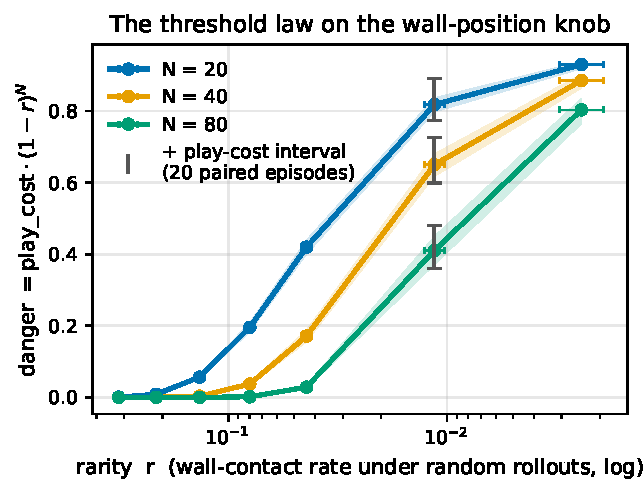
\includegraphics[width=0.55\textwidth]{figures/danger_threshold.pdf}
\caption{The threshold law on the wall-position knob (Table~\ref{tab:danger} rendered): danger $\approx 0$ while the wall is inside the random envelope, rises through the elbow, plateaus at full play\_cost; $N$ shifts the threshold.}
\label{fig:threshold}
\end{figure}

\begin{figure}[ht]
\centering
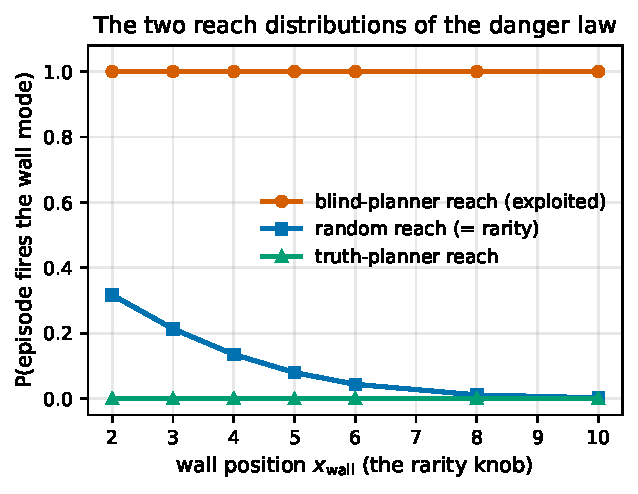
\includegraphics[width=0.55\textwidth]{figures/reach_mechanism.pdf}
\caption{The two reach distributions of the danger law: the exploited planner's mode reach is flat at 1.00 across the knob; random reach (= rarity) falls two orders of magnitude; the truth planner's trajectory reach is 0.00 --- the mode lives on its \emph{query} distribution (Proposition~\ref{prop:playcost}), not its path.}
\label{fig:reach}
\end{figure}

Readings: \textbf{the threshold law again} --- danger $\approx 0$ while the wall sits inside the random-rollout envelope, rises through the elbow, and plateaus at full play\_cost, with the entire elbow inside the sweep (Figure~\ref{fig:threshold}). \textbf{play\_cost is knob-invariant and $\approx 1$} (exceeding 1 at every knob except the largest, where far-plateau leakage gives 0.977): the blind planner is not merely uninformed but \emph{exploited} --- MPC on the wall-less model plans into the phantom region, is pinned at the wall (final $x = x_\mathrm{wall}$ exactly, contact rate 1.00 at every knob), and replans the same doomed plan every step, for the entire episode, scoring below random at every knob but the largest (0.00 vs 0.53). The 0.977 at $x_\mathrm{wall} = 10$ is the sigmoid tail of the far plateau leaking $J_\mathrm{blind} = 0.94$; the mechanism is unchanged. \textbf{The reach mechanism} appears in its cleanest form (Figure~\ref{fig:reach}), with the query/trajectory distinction now visible. Gate-miss exactness is re-verified in-tests and again at gate scale in Section~\ref{sec:axes}.

\paragraph{The residual leak is a reward artifact, not a mechanism fact --- measured, not argued.} At the widest knobs the pinned planner scores \emph{above} the uniform-random policy (cart $x_\mathrm{wall}=10$: $J_\mathrm{blind} = 0.94$ against $J_\mathrm{rand} = 0.53$; the three farthest pendulum stops likewise), which is why the claim above is ``exploited at every knob'' rather than ``below random at every knob''. The cause is the far plateau's sigmoid \emph{tail}: a planner pinned at $x = 10$ still collects $1/(1+e^{(12-10)/\mathrm{width}})$ per step, which at $\mathrm{width} = 0.5$ is $0.018$ and over 80 steps is most of $J_\mathrm{blind}$. A \textbf{sharp-plateau variant} (\texttt{scripts/continuous\_sharp\_plateau.py}, cart width $0.5 \to 0.2$, pendulum $0.25 \to 0.1$; sibling JSONs, the default instruments and every synthesis artifact untouched) removes the tail and settles it:
\begin{itemize}
\item \textbf{The exploitation claim strengthens.} On the cart the blind planner is below random at \textbf{7/7} knobs instead of 6/7, by two to thirteen orders of magnitude ($J_\mathrm{blind}$ from $2.3\times10^{-13}$ to $2.4\times10^{-3}$ against $J_\mathrm{rand} = 0.532$); on the pendulum, 5/6 instead of 3/6 --- and 6/6 with the asymmetric variant below.
\item \textbf{play\_cost becomes knob-invariant to ${\approx}1.5\times10^{-4}$}: cart $[1.0307, 1.0309]$ (spread $1.4\times10^{-4}$, against the default's $5.5\times10^{-2}$) and pendulum $[0.9999, 1.0000]$ (spread $1.5\times10^{-4}$, against $6.1\times10^{-2}$) --- a $400\times$ tightening on both, i.e.\ the invariance the default sweeps show approximately is exact once the tail is gone.
\item \textbf{It costs no planner competence}, the pre-registered risk: a sharper plateau gives random shooting less gradient to follow, yet $J_\mathrm{truth}$ moves only $17.77 \to 17.76$ (cart) and $20.08 \to 20.05$ (pendulum), and contact stays $1.00$ at every knob.
\item \textbf{The residue, and its fix.} Narrowing \emph{both} plateaus starves the random policy too ($J_\mathrm{rand}$ collapses to $3.6\times10^{-4}$ on the pendulum), which is why one knob there still reads above random: at $\theta_\mathrm{stop} = 2.0$, $J_\mathrm{blind} = 3.1\times10^{-3}$ against that collapsed baseline. The diagnosis says what to do --- narrow only the \emph{phantom} plateau, whose tail is what a pinned planner collects, and leave the real one at its default width. That variant ($\mathrm{width}_\mathrm{right} = 0.08$, per-plateau widths; \texttt{-{}-width-right}) gives \textbf{6/6} knobs below random: $J_\mathrm{blind}$ between $4.3\times10^{-4}$ and $7.1\times10^{-4}$ against a surviving $J_\mathrm{rand} \in [0.0572, 0.0584]$, with $J_\mathrm{truth}$ unchanged at $20.08$, contact $1.00$ everywhere, and play\_cost in $[1.0028, 1.0029]$ --- a spread of $7.1\times10^{-5}$, tighter still than the symmetric variant and $850\times$ tighter than the default. So on both instruments the strong form holds: exploited, pinned, and below random at \emph{every} knob, with play\_cost invariant to $10^{-4}$, once the phantom's tail is gone.
\end{itemize}
So the mechanism does not depend on the leak, and the knob-invariance claim is the one that sharpens: it is exact, not approximate, in the instrument without a tail.

\subsection{Robustness: the same law on a nonlinear plant}
\label{sec:pendulum}

The cart's off-mode dynamics are linear, which is convenient for Section~\ref{sec:smooth} but invites the worry that the phenomenology depends on it. A second instrument --- a pendulum (gravity term $\sin\theta$, $\theta = 0$ hanging down) with a hard angular stop, same interface, same MPC, same two-plateau reward on $\theta$ --- reproduces the identical picture with \emph{no} re-calibration (rarity is natural here: gravity confines the random walk near the bottom, so climbing to the stop is rare):

\begin{table}[ht]
\centering
\small
\begin{tabular}{rrrrrrr}
\toprule
$\theta_\mathrm{stop}$ & rarity & $J_\mathrm{truth}$ & $J_\mathrm{blind}$ & play\_cost & blind hit & d@40 \\
\midrule
0.8 & 0.2876 & 20.08 & 0.01 & 1.002 & 1.00 & 0.000 \\
1.0 & 0.1270 & 20.08 & 0.03 & 1.002 & 1.00 & 0.004 \\
1.2 & 0.0509 & 20.08 & 0.05 & 1.000 & 1.00 & 0.124 \\
1.4 & 0.0196 & 20.08 & 0.12 & 0.997 & 1.00 & 0.452 \\
1.6 & 0.0070 & 20.08 & 0.26 & 0.990 & 1.00 & 0.748 \\
2.0 & 0.0007 & 20.08 & 1.23 & 0.942 & 1.00 & 0.917 \\
\bottomrule
\end{tabular}
\caption{Pendulum-with-stop: threshold law, knob-invariant exploitation (pinned at the stop in every episode at every knob), truth planner untouched by the mode. The mechanism does not care that the plant is nonlinear --- only that the mode is hard and rare under the gate's measure. Rarity is the fraction of \textbf{30{,}000} random rollouts that fire the stop (Wilson 95\% CIs for every row in the versioned JSON). The sample was raised from 3000 specifically because the widest knob was a censored zero there ($0/3000$); at 30{,}000 it resolves to $0.0007$ $[0.0004, 0.0010]$, so every row is now a point estimate and every d@40 a number rather than a bound.}
\label{tab:pendulum}
\end{table}

\subsection{Two modes at once: a 4D bi-modal instrument}
\label{sec:patch2d}

Both instruments so far are one hard boundary in a 2D state. \textbf{PatchField2D} closes both structural gaps at once --- a 4D state and two independent modes --- and asks what the 1D instruments cannot: does the danger law compose mode-wise? State $(x, y, v_x, v_y)$; a \emph{scalar} action $a \in [-a_{\max}, a_{\max}]$ is mapped to a heading $\phi = \pi\,\mathrm{clamp}(a)/a_{\max}$ so all planner machinery (which consumes scalar actions) is reused unchanged; semi-implicit Euler:
\[
v_x' = v_x + (\mathrm{gain}\cos\phi - \mathrm{drag}\,v_x)\,dt, \quad
v_y' = v_y + (\mathrm{gain}\sin\phi - \mathrm{drag}\,v_y)\,dt,
\]
$x' = x + v_x'\,dt$, $y' = y + v_y'\,dt$. The two \textbf{modes} are circular sticky patches $P_i = \mathrm{disc}(c_i, R)$: if $(x', y') \in P_i$ the next state is $(x, y, 0, 0)$ --- the probe stops inelastically at its \emph{previous} position with zero velocity (the 2D analogue of the wall clamp, and the structure the 2D mitigation exploits, Section~\ref{sec:patch2d-mitigation}). Reward is two radial sigmoid lodes, a small real one near the start and a large phantom one behind the patches; the mode-blind planner aims straight at the phantom and freezes at a patch edge. The two knobs are the patch centers' distances along and off the start-to-lode corridor ($k_1$ the near patch, $k_2$ the far one); defaults are frozen once, never tuned per cell.

Table~\ref{tab:patch2d} sweeps the $3\times3$ knob grid (\texttt{scripts/continuous\_patch2d.py}; 600 rarity rollouts and 20 MPC episodes/arm per cell). The per-mode rarities separate cleanly ($r_1 \in [0.085, 0.245]$, $r_2 \in [0.0067, 0.0100]$), $J_\mathrm{blind} = 0$ at every cell (the blind planner freezes at a patch edge every episode; $J_\mathrm{rand} = 0.11$), and play\_cost is knob-invariant at $[1.005, 1.006]$ --- the same below-random exploitation as the 1D instruments, now on a 4D plant. \textbf{The danger law applies per mode and to the pair --- but it does not \emph{factor}.} Proposition~\ref{prop:gatemiss} holds for any measurable critical event, so the per-mode gate-miss factors are $(1-r_i)^N$ and the joint one is $(1-r_\cup)^N$, where $r_\cup$ is the probability that a rollout contacts \emph{either} patch (Proposition~\ref{prop:jointmiss}). We \emph{measure} $r_\cup$ rather than compose it: writing the joint factor as the product $(1-r_1)^N(1-r_2)^N$ would assume the two per-mode contact events are independent within a rollout, and they are not. At 600 rollouts $P(\text{both})$ is only $0$ to $3$ counts per knob, so the product's $-17\%$ to $+12\%$ relative error across this grid is not by itself evidence of anything: six of the nine cells are censored zeros, which force the product to over-estimate by construction. The dependence was therefore re-measured at $50{,}000$ rollouts on four knobs (\texttt{scripts/\allowbreak patch2d\_\allowbreak dependence\_\allowbreak 50k.py}), where it \emph{is} resolvable and does change direction: negative at $(2,6)$ and $(3,7)$, positive at $(4,6)$, all three with Wilson intervals excluding $r_1r_2$, and undecided at $(4,7)$. The mechanism is visible in the sign: a rollout that freezes at the near patch has spent its travel (negative), while reaching a far patch usually means passing the near one (positive). Both columns are in the versioned JSON (\texttt{d40\_joint} and \texttt{d40\_joint\_indep\_approx}); the table reports the measured one. Three honest notes: the $r_2$ knob is only weakly resolved at 600 rollouts (its trend is under-resolved, not flat), the $k_1{=}4$ one-hit bump in $r_2$ is sampling noise rather than a knob effect, and the four-decimal \texttt{d@40} figures in the $P_2$ and joint columns inherit that resolution --- at $4$ to $6$ hits in $600$ the interval on $\mathrm{d@40}\,P_2 = 0.7700$ is $[0.51, 0.91]$, so those digits are bookkeeping, not precision.

\begin{table}[ht]
\centering
\small
\begin{tabular}{rrrrrrrrrr}
\toprule
$k_1$ & $k_2$ & $r_1$ & $r_2$ & $r_\cup$ & $J_\mathrm{truth}$ & play\_cost & d@40 $P_1$ & d@40 $P_2$ & d@40 joint \\
\midrule
2 & 6 & 0.2450 & 0.0100 & 0.2517 & 17.98 & 1.006 & 0.0000 & 0.6732 & 0.0000 \\
2 & 7 & 0.2450 & 0.0083 & 0.2533 & 18.02 & 1.006 & 0.0000 & 0.7200 & 0.0000 \\
2 & 8 & 0.2450 & 0.0067 & 0.2517 & 18.08 & 1.006 & 0.0000 & 0.7700 & 0.0000 \\
3 & 6 & 0.1417 & 0.0083 & 0.1500 & 18.57 & 1.006 & 0.0022 & 0.7197 & 0.0015 \\
3 & 7 & 0.1417 & 0.0083 & 0.1500 & 18.47 & 1.006 & 0.0022 & 0.7197 & 0.0015 \\
3 & 8 & 0.1417 & 0.0067 & 0.1483 & 17.72 & 1.006 & 0.0022 & 0.7699 & 0.0016 \\
4 & 6 & 0.0883 & 0.0083 & 0.0917 & 20.85 & 1.005 & 0.0249 & 0.7192 & 0.0215 \\
4 & 7 & 0.0883 & 0.0100 & 0.0950 & 19.52 & 1.006 & 0.0249 & 0.6727 & 0.0185 \\
4 & 8 & 0.0850 & 0.0083 & 0.0933 & 19.08 & 1.006 & 0.0288 & 0.7196 & 0.0200 \\
\bottomrule
\end{tabular}
\caption{PatchField2D mechanism sweep ($3\times3$ knobs; 600 rarity rollouts, 20 MPC episodes/arm; $J_\mathrm{blind} = 0$, $J_\mathrm{rand} = 0.11$ at every cell). d@40 $P_i$ = $\mathrm{play\_cost}\cdot(1-r_i)^{40}$ (per-mode danger); $r_\cup$ = measured probability that a rollout contacts either patch; d@40 joint = $\mathrm{play\_cost}\cdot(1-r_\cup)^{40}$, the danger law at the joint critical event --- \emph{not} the product $((1-r_1)(1-r_2))^{40}$, which would assume within-rollout independence and errs by $-17\%$ to $+12\%$ here. Full table (with $J_\mathrm{blind}$, $J_\mathrm{rand}$, hit rates) in \texttt{docs/EXPERIMENTS.md}.}
\label{tab:patch2d}
\end{table}

\subsection{A second planner family: play\_cost is planner-dependent}
\label{sec:cem}

Proposition~\ref{prop:playcost} bounds play cost by the planner's query-hit probability on the disagreement region: a blind model can change behavior only to the extent that the planner queries where it is wrong. That is an upper bound and therefore only one implication --- low query reach forces low play cost; high query reach permits but does not force high play cost --- so ``two branches'' below names two \emph{measured} regimes that sit at the two ends of the bound, not a dichotomy the proposition predicts. Random-shooting MPC's constant candidates reach the distant phantom plateau in imagination and produce play\_cost ${\approx}1$. We repeated the full 11-knob grid with a second base planner, the cross-entropy method (CEM; \texttt{scripts/continuous\_cem.py}; horizon 40, 5 iterations, 64 samples, elite fraction 0.125, minimum standard deviation 0.05; one fixed setting across both instruments). The crossing columns in Table~\ref{tab:cem} are the fraction of sampled imagined trajectories that cross the omitted boundary, measured for BOTH planners with one plan from the same paired initial state per episode seed (episode-accumulated CEM fractions, which tell the same story, are recorded in the results JSON).

\begin{table}[ht]
\centering
\small
\begin{tabular}{lrrrrrr}
\toprule
instrument & knob & pc MPC & pc CEM & contact CEM & crossing CEM & crossing MPC \\
\midrule
cart & 2.0 & 1.031 & 0.000 & 0.00 & 0.0309 & 0.3865 \\
cart & 4.0 & 1.031 & 0.000 & 0.00 & 0.0055 & 0.2453 \\
cart & 6.0 & 1.031 & 0.000 & 0.00 & 0.0003 & 0.1483 \\
cart & 8.0 & 1.030 & 0.000 & 0.00 & 0.0000 & 0.0773 \\
cart & 10.0 & 0.977 & 0.000 & 0.00 & 0.0000 & 0.0369 \\
pendulum & 0.8 & 1.002 & 0.009 & 0.70 & 0.1150 & 0.6392 \\
pendulum & 1.0 & 1.002 & 0.025 & 0.25 & 0.0483 & 0.5530 \\
pendulum & 1.2 & 1.000 & $-0.011$ & 0.00 & 0.0164 & 0.4672 \\
pendulum & 1.4 & 0.997 & $-0.021$ & 0.00 & 0.0053 & 0.3842 \\
pendulum & 1.6 & 0.990 & $-0.021$ & 0.00 & 0.0013 & 0.3039 \\
pendulum & 2.0 & 0.942 & 0.000 & 0.00 & 0.0002 & 0.2158 \\
\bottomrule
\end{tabular}
\caption{The same certified-blind models under two base planner families (20 paired episodes/row). ``pc'' is blind-model play\_cost within that planner family; crossing is the sampled imagined-boundary-crossing proxy for query-hit mass, one plan per episode seed from paired initial states for both planners. CEM stays near zero play cost and below MPC's crossing fraction on every row.}
\label{tab:cem}
\end{table}

CEM's blind-model play cost lies in $[-0.0213,0.0248]$ on every row --- and the seed-paired 95\% t-interval includes zero on all 11 rows --- while its imagined crossing fraction is strictly below MPC's throughout. Two of those eleven intervals deserve their asterisk. On the five cart rows every per-seed difference is $0.0$ exactly, so the interval is degenerate $[0,0]$ and ``includes zero'' is a restatement of bit-identity rather than an inference; we report it as bit-identity in the prose for that reason. On the pendulum rows the standard deviation is inflated roughly fortyfold by one seed (index 16, differences $-0.427$ to $-0.423$ across three knobs), so the interval is a real interval but its width is that outlier's, not a noise scale. On the cart, truth- and blind-model CEM returns are identical and contact is zero everywhere. The nearest pendulum stops are an honest qualification: CEM contacts $\theta_\mathrm{stop}=0.8$ in 70\% of episodes and $1.0$ in 25\%, but does not enter MPC's pinned, below-random regime; contact is zero from $\theta_\mathrm{stop}\geq1.2$. Contact is therefore not itself exploitation. One caveat before crediting Proposition~\ref{prop:playcost} with this. The bound is in terms of $\mu_{\mathrm{query}}(E)$, the probability that \emph{at least one} query in an episode lands in the disagreement region, whereas the crossing column is the \emph{fraction} of imagined candidates that cross. With ${\sim}200$ candidates $\times$ 40 imagined steps per replan, any nonzero crossing fraction makes $\mu_{\mathrm{query}}(E) \approx 1$ and the bound $\lesssim 1$ --- true but vacuous. So only the two rows with crossing \emph{exactly} $0$ (cart $x_\mathrm{wall} = 8, 10$) genuinely instantiate the bound's low-reach branch, where $\mu_{\mathrm{query}} = 0$ forces $\mathrm{play\_cost} = 0$ and CEM delivers it. On the remaining nine rows the near-zero play cost is consistent with the proposition but not explained by it: it is an empirical planner-dependence result, and the crossing fraction is a \emph{proxy} for query reach rather than the quantity the bound constrains. What survives in either reading is Section~\ref{sec:lessons}'s first lesson --- if search does not discover the phantom, it cannot optimize toward it.

Two caveats prevent the wrong conclusion. CEM's pendulum truth return varies from 15.36 to 16.46 (versus MPC's 20.08), consistent with local optima; the comparison is blind-CEM against truth-CEM, not a claim that CEM is globally optimal. And limited reach is not knowledge or mitigation: a planner that misses a phantom distant reward can also miss a real one. This is one fixed CEM configuration, not a hyperparameter sweep.

\textbf{PatchField2D: the anticipated 2D competence gap did not materialize.} On the 4D bi-modal instrument (\texttt{scripts/continuous\_cem\_patch2d.py}) blind CEM is again \emph{not} exploited: play\_cost is $-0.022 / {+}0.017 / {+}0.020$ at knobs $(2,6)/(3,7)/(4,8)$ with the seed-paired 95\% $t$-interval including zero on all three rows, and CEM's imagined crossing fraction is below MPC's on every row ($0.070 < 0.208$, $0.027 < 0.149$, $0.009 < 0.094$). Here CEM is \emph{competent in aggregate} --- the 2D competence gap we anticipated did not appear --- but with per-seed variance (one truth-CEM episode at $\approx 0.97$), and its blind contact rate is a uniform $0.05$ (nonzero, unlike the cart's $0.00$, and without positive play cost). The same low-query-reach branch of Proposition~\ref{prop:playcost}, one more instrument.

\section{Axis separation: the gate fails only where the law says it can}
\label{sec:axes}

The classic continuous-model failure axis is pervasive sub-tolerance error; the danger law's axis is a localized hard mode. A tolerance gate ($\varepsilon = 0.01$, deployment-realistic) must be shown to fail \emph{only} on the second axis, and only at the $(1-r)^N$ rate. Five arms, one table (\texttt{scripts/continuous\_axes.py}; reveal-rarity $=$ P(a random rollout contains a transition where truth and model differ $> \varepsilon$), 20{,}000 rollouts; pass@40 over 300 independent $N{=}40$ gates; 20 MPC episodes/arm). For the hard mode, the mode-firing rarity of Tables~\ref{tab:danger}--\ref{tab:pendulum} and the reveal-rarity here coincide as events --- the mode error exceeds every deployment-realistic $\varepsilon$ (the $\varepsilon$-sweep below), so a rollout fires the mode iff it reveals a disagreement --- which licenses the shared symbol $r$.\footnote{With both samples raised, the two estimates of the same event now agree to the third decimal: mode-firing rarity $0.1352$ on 30{,}000 rollouts (Table~\ref{tab:danger}) against reveal-rarity $0.1351$ on 20{,}000 (Table~\ref{tab:axes}). At the earlier sample sizes they read $0.1430$ and $0.1385$ --- the gap was resampling noise, as this now confirms rather than asserts.}

\begin{table}[ht]
\centering
\small
\begin{tabular}{lrrrrr}
\toprule
arm & reveal-rarity & $(1-r)^{40}$ & pass@40 measured & play\_cost & d@40 \\
\midrule
wall@4 omitted & 0.1351 & 0.0030 & 0.003 & 1.031 & 0.0031 \\
wall@8 omitted & 0.0103 & 0.6622 & 0.667 & 1.030 & 0.6821 \\
drag bias $\times$1.03 (sub-$\varepsilon$) & 0.0001 & 0.9940 & 0.997 & 0.000 & 0.0000 \\
drag bias $\times$2.0 (supra-$\varepsilon$) & 1.0000 & 0.0000 & 0.000 & 0.000 & 0.0000 \\
$C^\infty$ bump@4, amp 0.5 & 0.1829 & 0.0003 & 0.000 & 0.000 & 0.0000 \\
$C^\infty$ bump@4, amp 1.0 & 0.2018 & 0.0001 & 0.000 & $-0.745$ & $-0.0001$ \\
\bottomrule
\end{tabular}
\caption{Axis separation at $\varepsilon = 0.01$, $N = 40$; d@$N$ = $\mathrm{play\_cost}\cdot(1-r)^N$, as in Table~\ref{tab:danger}. Danger lives in one quadrant only: rare $\wedge$ hard-mode. Reveal-rarity is measured on \textbf{20{,}000} rollouts (raised from 2000 because the sub-$\varepsilon$ arm was a censored zero there): it now resolves to $0.0001$, and its predicted pass rate $0.9940$ sits inside the measured $[0.9814, 0.9994]$ instead of above it.}
\label{tab:axes}
\end{table}

\begin{figure}[ht]
\centering
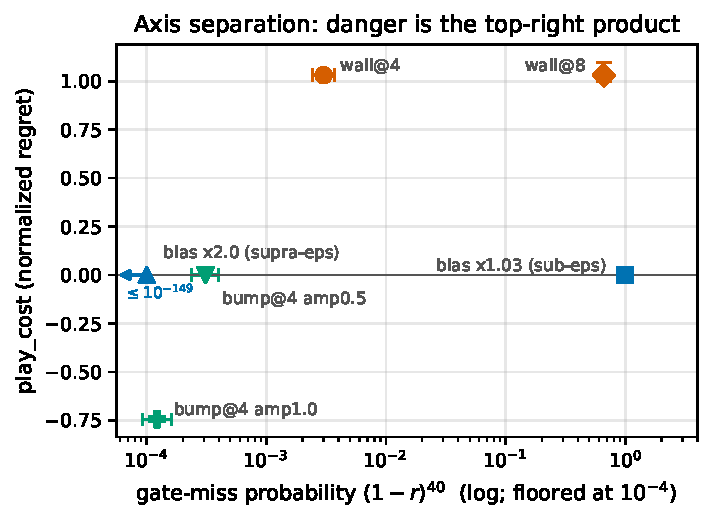
\includegraphics[width=0.6\textwidth]{figures/axis_separation.pdf}
\caption{Table~\ref{tab:axes} as the danger quadrant: gate-miss probability (log) vs play\_cost. Only the rare hard mode reaches the top right; danger is the product of the coordinates.}
\label{fig:axes}
\end{figure}

Readings (Table~\ref{tab:axes}, rendered as the danger quadrant in Figure~\ref{fig:axes}): \textbf{gate exactness at gate scale} --- measured pass@40 matches $(1-r)^{40}$ in both wall rows --- 0.003 vs 0.0030 and 0.667 vs 0.6622, each prediction inside the 300-gate Wilson interval. Two bookkeeping points that we got wrong before and that matter for reading any of these agreements. First, $\hat r$ carries its own error, and the prediction $(1-\hat r)^{40}$ inherits it: propagating the rarity's Wilson interval, the $20{,}000$-rollout reveal-rarity $0.01025$ $[0.00895, 0.01174]$ predicts a pass rate in $[0.623, 0.698]$, which contains the measured $0.667$. Once that propagation is done, the earlier ``marginal failure'' on $2000$ rollouts dissolves: $\hat r = 0.0125$ $[0.0085, 0.0184]$ there predicts $[0.476, 0.711]$, comfortably containing $0.667$ --- so the old $0.6046$ point estimate was never below the interval in any meaningful sense; it was a point compared against an interval while its own interval went unquoted. Second, this instrument has \emph{two} rarity estimates for what Proposition~\ref{prop:epsinv} says is one event: $0.01140$ from the $30{,}000$-rollout mode-firing sweep of Table~\ref{tab:danger} (predicting $0.632$) and $0.01025$ from the $20{,}000$-rollout reveal-rarity here (predicting $0.662$). Their intervals overlap and the proposition says the events coincide below $\varepsilon^\star$, so this is sampling noise and not a contradiction --- but the $10\%$ relative gap is larger than either interval's half-width suggests one should ignore, and we quote the reveal-rarity throughout this table and the firing rarity throughout Table~\ref{tab:danger} rather than mixing them. The proposition is the observed acceptance rate, not asymptotic decoration. \textbf{The gate polices the pervasive axis}: a global drag bias above tolerance is revealed on every rollout and never accepted; a sub-tolerance bias is accepted at 0.997 --- which the law now \emph{predicts} rather than excuses: that arm does reveal a disagreement on a thin slice of rollouts (reveal-rarity $0.0001$, the extreme velocity tail), for a predicted pass rate of $0.9940$ --- and it is harmless at play. Verified-and-fine is a real cell, and the gate finds it. \textbf{Smoothness kills consequence, not detectability}: the $C^\infty$ drag bump at the wall's location has comparable rarity to the wall (0.18 vs 0.14 --- it is just as \emph{detectable}, confirming Proposition~\ref{prop:lipschitz} is about error geometry, not about hiding from the gate, and matching the direction of Proposition~\ref{prop:detectrate}) yet play\_cost 0.000 at amplitude 0.5. At amplitude 1.0 play\_cost turns \emph{negative} ($-0.745$): the truth planner, seeing the slowdown near its horizon edge, is over-pessimistic and often settles for the small plateau, while the bump-blind planner pushes through and wins. A smooth localized omission produces planner-side timing effects of ambiguous sign; only the hard mode produces the one-way exploitation geometry (pinned, forever, below random).

\textbf{Is $\varepsilon = 0.01$ a special setting, or is the axis separation itself $\varepsilon$-invariant?} A sweep over $\varepsilon \in \{10^{-9}, 10^{-6}, 10^{-4}, 10^{-3}, 10^{-2}, 3{\times}10^{-2}, 0.1, 0.3\}$ (\texttt{scripts/continuous\_eps\_sweep.py}; Table~\ref{tab:eps-sweep} for the cart, full grid in \texttt{docs/EXPERIMENTS.md}) answers: $\varepsilon$-invariant. Mode-arm reveal-rarity is flat across the entire deployment-realistic range --- on the cart, \texttt{wall@8} is bit-identically flat through the whole grid including $\varepsilon = 0.3$, and \texttt{wall@4} only dips slightly (never widens) at the top of the grid. The pervasive bias arms switch sharply at their own error scale on both instruments instead.

\begin{table}[ht]
\centering
\small
\begin{tabular}{rrrr}
\toprule
$\varepsilon$ & wall@8 rarity & bias $\times$1.03 rarity & bias $\times$2.0 rarity \\
\midrule
$10^{-6}$ & 0.0125 & 1.0000 & 1.0000 \\
$10^{-2}$ & 0.0125 & 0.0000 & 1.0000 \\
0.1 & 0.0125 & 0.0000 & 0.0040 \\
0.3 & 0.0125 & 0.0000 & 0.0040 \\
\bottomrule
\end{tabular}
\caption{Reveal-rarity vs. $\varepsilon$ (cart). The mode arm is flat across the whole grid; the pervasive arms switch at their own error scale.}
\label{tab:eps-sweep}
\end{table}

The pendulum replicates both halves: its mode arms are flat too (only a slight dip at the top of the grid --- \texttt{stop@1.0} rarity 0.1410 at $\varepsilon \le 3{\times}10^{-2}$, dipping to 0.1400 at $\varepsilon = 0.1$ and 0.1240 at $\varepsilon = 0.3$), and its bias arms switch at the same error-scale boundaries as the cart's. pass@40 $\approx (1-r)^{40}$ continues to hold for the mode arms at every $\varepsilon$ in the grid, on both instruments. (The sweep's own rarity column is measured on 2000 rollouts per cell, since what it has to establish is \emph{flatness in $\varepsilon$} rather than a third digit; the 20{,}000-rollout estimate of the same quantity in Table~\ref{tab:axes} is $0.0103$ against this sweep's $0.0125$, one estimate's noise apart. An earlier version of this note recorded the closed-form prediction sitting marginally below the empirical Wilson lower bound; with the rarity re-measured on 20{,}000 rollouts that gap closes.) play\_cost is not re-measured across $\varepsilon$: the model under test does not depend on the gate's tolerance, so play behavior is $\varepsilon$-independent by construction --- the sweep varies only what the gate can see. The gate's $\varepsilon$ is a pervasive-error dial, not a mode-detection dial: tightening it cannot catch the hard mode, and loosening it does not widen the hole.

\textbf{The 4D bi-modal instrument replicates the flat mode arm, once per mode.} On PatchField2D the $\varepsilon$-sweep (\texttt{scripts/continuous\_eps\_sweep\_patch2d.py}) gives \emph{exactly} flat mode-arm reveal-rarity across the entire grid: patches-omitted $0.147$, patch-1-only $0.142$, patch-2-only $0.005$ --- each constant at every $\varepsilon$. The per-mode arms recover the per-mode rarities of the mechanism sweep (Section~\ref{sec:patch2d}), so the tolerance axis is orthogonal to the mode hole on the bi-modal instrument too, and separately for each mode.

\section{Mitigation: the exploitation is planner-mediated}
\label{sec:mitigation}

The exploitation measured in Sections~\ref{sec:mechanism} and~\ref{sec:axes} is planner-mediated, not model-mediated, and a planner-side fix collapses it without touching the model or the gate --- this does \textbf{not} contradict the danger law (the gate still certifies a wrong model; Proposition~\ref{prop:ident} is untouched). Like those sections, this one uses the hand-written instruments and blind models, not LLM synthesis. Distrust-region replanning (\texttt{src/cwm/continuous/mitigation.py}, strictly additive) compares the model's prediction against the observed transition after every real step ($\mathrm{tol} = 10^{-6}$); a disagreement records the \emph{position of the model's refuted prediction} --- not the pre-state --- as a one-sided fence, since false predictions always lie on or beyond the mode boundary. While scoring a candidate rollout, the first imagined step whose position interval crosses a fence's $\varepsilon$-band ($\varepsilon = 0.25$ cart, $\varepsilon = 0.1$ pendulum) truncates the rollout --- reward kept, everything downstream dropped --- which makes the fence leap-proof at any imagined speed; candidates are then ranked by (truncated return, distance to the nearest fence), which structurally prefers the real side \emph{in one dimension}. The qualifier is load-bearing and we had dropped it: the tie-break is an unsigned distance, so in 1D, where the fence lies beyond the boundary and the real side is the only other direction, maximizing it flees the mode --- but in 2D it is symmetric between rounding the patch and plunging through it, and Section~\ref{sec:patch2d-mitigation} measures what that costs. With zero violations this is bit-identical to plain MPC by construction (tested bitwise) --- mitigation costs nothing when the model is right. Only this design is undodgeable: three earlier attempts (pre-state flee-balls; full-state point fences, dodged by the planner probing crossing velocities) were each defeated by the argmax planner acting as an adversary against the fence. The collapse is scoped to \textbf{hard-boundary hybrid modes}: the one-sided fence works precisely because a refuted prediction lies on or beyond the mode boundary, so fencing its far side cannot cut off any real trajectory. This structural fact is what these wall/stop instruments supply; less structured failure modes (soft or moving boundaries, errors not confined to a hard stop) do not obviously admit such a fence and are untested --- this is a hard-boundary mitigation, not yet a general planner-side one.

\begin{table}[ht]
\centering
\small
\begin{tabular}{lrrr}
\toprule
knob & pc\_blind & pc\_mit & first-contact step \\
\midrule
\multicolumn{4}{l}{\emph{cart} ($x_\mathrm{wall}$)} \\
2  & 1.031 & 0.290 & 11.6 \\
4  & 1.031 & 0.446 & 16.9 \\
6  & 1.031 & 0.578 & 21.3 \\
8  & 1.030 & 0.699 & 25.1 \\
10 & 0.977 & 0.806 & 28.7 \\
\multicolumn{4}{l}{\emph{pendulum} ($\theta_\mathrm{stop}$)} \\
0.8 & 1.002 & 0.113 & 7.0 \\
1.0 & 1.002 & 0.129 & 8.1 \\
1.2 & 1.000 & 0.143 & 9.0 \\
1.4 & 0.997 & 0.160 & 10.0 \\
1.6 & 0.990 & 0.177 & 11.0 \\
2.0 & 0.942 & 0.212 & 13.0 \\
\bottomrule
\end{tabular}
\caption{Mitigation sweep (20 episodes/knob, both instruments). pc\_blind / pc\_mit = play\_cost of the blind planner under plain MPC / under distrust-region mitigation. Full 11-row table with contact rates and violation counts in \texttt{docs/EXPERIMENTS.md}.}
\label{tab:mitigation}
\end{table}

The collapse is large at every knob (Table~\ref{tab:mitigation}): \texttt{pc\_blind} stays pinned at $\approx 0.94$--$1.03$ everywhere (established in Section~\ref{sec:mechanism}, Tables~\ref{tab:danger} and~\ref{tab:pendulum}), while \texttt{pc\_mit} never exceeds $0.81$. Exactly one violation suffices to fence the mode on \emph{every} one of the 11 rows --- the mitigated planner must touch the mode once, which is identifiability operationalized: you cannot avoid what you have never seen. The residual \texttt{pc\_mit} is the honest cost of that unavoidable first contact, and it grows with the lure distance, read off the first-contact step: cart $0.290 \to 0.806$ as first contact goes $11.6 \to 28.7$ of 80 steps (knob $2 \to 10$); pendulum $0.113 \to 0.212$ as first contact goes $7.0 \to 13.0$ (knob $0.8 \to 2.0$). The cart knob $=10$ row is the least favorable in the sweep (\texttt{pc\_mit} $0.806$, close to blind's $0.977$) because the transient consumes most of the horizon --- but the blind planner stays pinned \emph{forever} there ($J$ $0.94$ of $J_\mathrm{truth}$ $17.77$) while the mitigated planner escapes and recovers most of the horizon ($J$ $3.88$): the normalized cost looks modest, the actual return does not.

\paragraph{Why exactly one violation, and what sets the count in general.} The single-violation sufficiency is not a lucky measurement either --- it is a covering number equal to one.

\begin{proposition}[the mitigation's new-coverage violations are bounded by a packing number]
\label{prop:fencecover}
Run distrust-region replanning with band $\varepsilon$. Let $F$ be the \emph{fence locus} --- the set of points at which a violation can record a fence, i.e.\ the possible refuted predictions --- and let $B$ be the \emph{entry barrier}, the set of points at which an imagined trajectory can enter the mode region. Two conclusions, with different hypotheses. (i) With no hypothesis at all, the number of violations that place a fence farther than $\varepsilon$ from every fence already placed is at most $N_{\mathrm{pack}}(F,\varepsilon)$, the $\varepsilon$-packing number of $F$, and $N_{\mathrm{pack}}(F,\varepsilon) \leq N_{\mathrm{cov}}(F,\varepsilon/2)$. (ii) If moreover $B \subseteq F \oplus B_\varepsilon$ --- every barrier point within $\varepsilon$ of some fenceable point --- then once the accumulated fences $\varepsilon$-cover $B$, no further violation occurs at all.
\end{proposition}

\begin{proof}
Fences placed farther than $\varepsilon$ from all their predecessors are pairwise more than $\varepsilon$ apart, so they form an $\varepsilon$-packing of $F$ and there are at most $N_{\mathrm{pack}}(F,\varepsilon)$ of them; for the comparison, a $(\varepsilon/2)$-ball has sup-diameter $\varepsilon$ and so contains at most one packing point, giving (i) with no hypothesis used. For (ii): once the fences $\varepsilon$-cover $B$, every imagined trajectory entering the mode region crosses $B$ within $\varepsilon$ of a fence and is truncated, so no candidate scores the phantom and no further violation occurs --- which is where the hypothesis $B \subseteq F \oplus B_\varepsilon$ is used, since otherwise no set of fences on $F$ can cover $B$.
\end{proof}

Two things in that statement are weaker than an earlier version of it, and both were forced by counterexample rather than caution. The bound is a \emph{packing} number, not a covering number. A covering number counts an \emph{optimal} cover, and the planner is not optimal --- it is explicitly an adversary against the fence --- so it can place every point of a maximal packing before the balls start pre-empting one another. On the unit circle at $\varepsilon = 0.5$ that is $12$ points, pairwise chord distance $0.5176 > \varepsilon$, and a grid sweep confirms every one of the $12$ adds coverage the others had not: $12$ against a covering number of $7$ (\texttt{scripts/\allowbreak circle\_\allowbreak covering\_\allowbreak number.py}). And the count is of \emph{new-coverage} fences only. Duplicates --- fences within $\varepsilon$ of an existing one --- are not bounded by this argument at all, and in our own data they dominate the tail: one episode records $28$ violations of which $24$ are at an identical point.

The two instrument families instantiate the two extremes of that bound.
\begin{itemize}
\item \textbf{1D: the measured $1.00$ is separation, not covering.} A position or angular clamp has a single boundary point, and Table~\ref{tab:mitigation} measures a mean of exactly $1.00$ violations on all eleven rows. We first read that as the covering bound at $N_{\mathrm{cov}} = 1$ being tight. It is not, and checking the instrument says so plainly (\texttt{scripts/\allowbreak fence\_\allowbreak separation\_\allowbreak census.py}): the fence is recorded at the model's refuted \emph{prediction}, which overshoots the wall by $0.17$ to $0.58$ against a band of $\varepsilon = 0.25$, so the band fails to contain $x_\mathrm{wall}$ in four of five cart episodes --- and the count is $1$ anyway. A hypothesis that fails while its conclusion holds is not the explanation.

  What is doing the work is that in one dimension a single point beyond the boundary \emph{disconnects} the agent from the phantom: every imagined path to the lure crosses it, so the segment test truncates all of them, wherever in the far region the fence landed. That mechanism has a signature the covering story does not --- insensitivity to $\varepsilon$ --- and it holds where we can measure it: sweeping $\varepsilon$ over a $20\times$ range on the pendulum ($0.1$ down to $0.005$) leaves the returns and violation counts \emph{bit-identical}, and on the cart they are identical from $0.25$ down to $0.05$. It is not unconditional: at $\varepsilon = 0.01$ two of four cart seeds record a second violation, the strip between the boundary and the fence having grown wide enough for a real contact that no imagined segment crosses. So the honest 1D statement is a separation fact with a measured range of validity, not a covering number of $1$. The topological contrast with 2D is then the real one: removing one arc leaves a circle connected, so no single fence can separate a disc patch's inside from its outside, and the cut number jumps from $1$ to $2$ before any metric question arises.
\item \textbf{2D: the bounded quantity is the \emph{distinct} fence count, and it is a quarter of the budget.} A disc patch of radius $R$ has its fence locus inside the disc and its entry barrier on $\partial\,\mathrm{disc}$. A fence at a boundary point $\varepsilon$-covers an arc of angular width $4\arcsin(\varepsilon/2R)$, so a circle's packing number at $R = 1$, $\varepsilon = 0.5$ is $\mathbf{12}$ and its covering number is $7$ (both brute-force verified in \texttt{scripts/\allowbreak circle\_\allowbreak covering\_\allowbreak number.py}, which also exhibits the 12-point sequence and checks that one fewer ball does not cover). PatchField2D is \emph{bi-modal}, so the budget for an episode that touches both patches is $24$, not $12$ --- an earlier draft used one circle's worth.

  Against that budget, what the proposition bounds is the number of \emph{new-coverage} fences, and measuring it per episode (\texttt{scripts/\allowbreak fence\_\allowbreak separation\_\allowbreak census.py}) settles a claim we had got wrong twice. The distinct fence count never exceeds $2 / 5 / 6$ at knobs $(2,6)/(3,7)/(4,8)$ --- at most a quarter of the $24$-fence budget, not the ``about two thirds'' an earlier draft inferred. The raw violation counts are much larger and are dominated by \emph{duplicates}: the two worst episodes record $28$ violations each while placing at most $6$ distinct fences, and the per-episode distribution is heavily skewed (medians $1 / 1 / 2$ against means $1.05 / 2.65 / 4.25$). Quoting a $20$-episode mean against a per-episode bound compared the wrong two quantities in the first place.

  The arc percentages that used to appear here ($17\% / 43\% / 68\%$ of the circle) are withdrawn: they were the violation count divided by the budget, i.e.\ saturation assumed and restated as a percentage, then used to explain the count. Measured directly as the angular spread of fence bearings per patch per episode, the median probed arc is $0\% / 0\% / 87\%$ --- zero at the two near knobs because the typical episode places a single fence, and large at the far knob because the few episodes that map the boundary map most of it. That is a different shape of claim than a smooth progression, and it is what the instrument does.

  (A metric packing number at \emph{fixed} radius is the relevant quantity because the algorithm fixes the band $\varepsilon$; it is a different question from the minimal \emph{good} cover of a circle by contractible arcs, which is $3$ with no radius constraint and is the nerve-theoretic object paper~3 builds on. The free-centre optimum of $6$ is a zero-slack tiling special to $\varepsilon = R/2$ and closed balls, so it should not be read as a robust constant.)
\end{itemize}
\begin{corollary}[the deployment \emph{fencing} cost is exponential in the boundary's dimension]
\label{cor:fencedim}
Proposition~\ref{prop:fencecover} is dimension-free --- its proof uses only packing and covering of $F$ --- so instantiating it needs only a packing number. If $F$ is a $p$-dimensional Lipschitz piece of diameter $D$, then $N_{\mathrm{pack}}(F,\varepsilon) \leq N_{\mathrm{cov}}(F,\varepsilon/2) = O\big((2D/\varepsilon)^{p}\big)$, so the number of new-coverage contacts the mitigation must pay before it closes the phantom off grows exponentially in the \emph{boundary's} dimension $p$ (not the state's). The packing correction changes the constant, not the order, which is why the dimensional reading survives it intact. A $p=2$ mode surface would cost $O((2D/\varepsilon)^2)$ --- the precise sense in which the \emph{danger} is dimension-free while the \emph{fencing} is not.

Two caveats on instantiating the exponent. The constant hides the parametrization's Lipschitz constant and $p$-volume, which matters here because the whole quantitative dispute is over a constant. And two data points ($p = 0$ and $p = 1$) cannot distinguish $(2D/\varepsilon)^p$ from any other function agreeing at $p \in \{0,1\}$; the exponential form is the theorem's, not the measurement's.
\end{corollary}

We use \emph{fencing} rather than \emph{repair} for this cost deliberately: repair in this paper means the LLM rewriting the model from data (Section~\ref{sec:patch2d-synthesis}, where it fails outright on 2D regions), and the fencing cost is a planner-side quantity that leaves the model untouched. The covering-number analogue that Section~\ref{sec:limitations} once listed as open now appears on \emph{both} sides: gate-side for Lipschitz pairs (Proposition~\ref{prop:coverage}) and mitigation-side as the fencing count here. The dimensional reading is the paper's own: the danger law's $(1-r)^N$ is dimension-free, but fencing a mode at deployment time costs a packing number of its fence locus, which grows with that locus's dimension.

\subsection{The 2D mitigation: a partial collapse, and lock-in at the far knob}
\label{sec:patch2d-mitigation}

The distrust-region fence generalizes to PatchField2D (\texttt{scripts/\allowbreak continuous\_\allowbreak mitigation\_\allowbreak patch2d.py}): fences are the 2D positions of refuted predictions, which lie \emph{inside} an unreachable patch (the stay-at-previous-position clamp forces a refuted prediction strictly inside the disc, so fencing it cannot cut off any real trajectory), and a candidate rollout truncates when an imagined step \emph{segment} passes within $\varepsilon$ of a fence (segment-to-point distance, leap-proof); the 1D code path is preserved \emph{behaviorally} bit-identically --- the generalization rewrote the shared internals, so this is pinned by tests rather than by the diff: the no-violation case reduces to plain MPC exactly, and the 1D mitigated episodes with violations are golden-pinned to the run the sweep used (\texttt{tests/test\_mitigation\_1d\_regression.py}). But the collapse is now \textbf{partial and decays with patch distance} (Table~\ref{tab:patch2d-mitigation}): \texttt{pc\_blind} $\approx 1.006$ falls to \texttt{pc\_mit} $0.257 / 0.541 / 0.862$ at knobs $(2,6)/(3,7)/(4,8)$, with mean violations $1.05 / 2.65 / 4.25$ (against the 1D instruments' clean $1.0$) and first contact at step $8.5 / 12.35 / 15.25$.

We described that as a \textbf{boundary-mapping transient} --- the planner rounding one fence disc, re-contacting the edge elsewhere, accreting fences along the probed arc. The per-episode data say something less flattering, and the difference matters because it is a different failure mode rather than a slower version of success. The distributions are skewed, not shifted: medians $1 / 1 / 2$ against those means, with two episodes recording $28$ violations. And a growing fraction of episodes end \emph{pinned} at blind-level return --- $0/20$, $2/20$, $\mathbf{7/20}$ across the three knobs --- with every episode of $\geq 5$ violations returning near zero. In those episodes the agent is frozen against a patch edge and re-violates at the same predicted point every remaining step: at $(4,8)$, one episode records $24$ consecutive fences at an identical position. The mechanism is the tie-break. With a fence a few hundredths away, every candidate truncates at the first imagined step, so the ranking falls through to distance-to-nearest-fence --- an \emph{unsigned} scalar, which in 1D can only mean fleeing the mode but in 2D is symmetric between rounding the patch and plunging through it. So the mitigation does not merely decay with distance: at the farthest knob it \emph{fails outright} in a third of episodes, and what remains of the decaying-transient reading is the near knob, where the median episode places one fence and the collapse is clean.

This is the honest scope of a \emph{hard-boundary} mitigation on a curved 2D mode: the one-sided fence is sound (a refuted prediction lies inside an unreachable patch, so fencing it cannot cut off a real trajectory) and it works where the geometry lets an unsigned tie-break point away from the mode. It does not survive a boundary the agent can be pinned against. Fixing that needs a \emph{signed} away-direction in 2D --- the fence's outward normal rather than its distance --- which is a design change we have not tested, not a re-tuning.

\begin{table}[ht]
\centering
\small
\begin{tabular}{rrrrr}
\toprule
$(k_1, k_2)$ & pc\_blind & pc\_mit & mean viol. & first contact \\
\midrule
$(2, 6)$ & 1.006 & 0.257 & 1.05 & 8.50 \\
$(3, 7)$ & 1.006 & 0.541 & 2.65 & 12.35 \\
$(4, 8)$ & 1.006 & 0.862 & 4.25 & 15.25 \\
\bottomrule
\end{tabular}
\caption{PatchField2D mitigation sweep (paired seeds). The collapse is partial and degrades with patch distance. Read the means with the distribution beside them: medians are $1/1/2$, maxima $2/28/28$, and the count is dominated by duplicate fences (at most $2/5/6$ \emph{distinct} positions per episode). The degradation is not a longer transient but a growing fraction of outright failures --- $0/20$, $2/20$, $7/20$ episodes end pinned at blind-level return (\texttt{scripts/\allowbreak fence\_\allowbreak separation\_\allowbreak census.py}).}
\label{tab:patch2d-mitigation}
\end{table}

\section{LLM synthesis: the danger collapses to pure identifiability}
\label{sec:synthesis}

Real-LLM arms (\texttt{scripts/continuous\_danger\_synthesis.py}; Azure GPT-5.x mini and large\footnote{\textbf{Exact models.} ``large'' is the Azure OpenAI deployment \texttt{gpt-5.4} and ``mini'' is \texttt{gpt-5.4-mini}, both at API version \texttt{2025-04-01-preview}; the cross-family arms are \texttt{Qwen/Qwen3-Coder-30B-A3B-Instruct} (Hugging Face Inference Providers router) and Claude Sonnet (agent-relayed, Section~\ref{sec:synthesis}). Every result JSON under \texttt{results/} records its own \texttt{model} field, so each number is attributable to a named deployment; the runs are dated 2026-07-07 to 2026-07-20 in the repository history. We write ``GPT-5.x'' in prose where the claim holds for both sizes.}; $N = 40$ training rollouts which double as the gate, as in the companion paper's sweep; $\varepsilon = 10^{-9}$ pinned-integrator gate; \textbf{20 seeds/cell on the headline $x_\mathrm{wall} = 8$ cell, both sizes} (the companion paper's standard); 6 MPC play episodes/seed; per-seed JSON with the synthesized code versioned in the repository). The contract pins the integrator (Section~\ref{sec:cartwall}'s equations, stated in the spec text, constants generated from the environment instance so they cannot drift); the \emph{full} arm includes the wall clause, the \emph{incomplete} arm omits it. Crucially, each seed logs whether the wall fired in its training sample --- the identifiability event that the companion paper could not condition on post hoc.

\paragraph{One design fact governs every pooled count in this paper.} The gate sample of seed index $i$ is drawn with rollout seed $10^4(i{+}1)$ \emph{independently of which model is being run} (\texttt{scripts/continuous\_danger\_synthesis.py}), so at every instrument and knob the mini and large arms are synthesized from the \emph{same} samples. Pooling the two sizes therefore doubles the number of \emph{synthesis draws}, not the number of independent gate samples: a pooled $k/2n$ is $n$ shared samples with two model draws each. Two consequences we hold to throughout. (i) Any empirical check of the gate-miss rate $(1-r)^N$ is a per-size statement --- the mode-absent/present split is a property of the sample, so it is \emph{identical} across sizes by construction and cannot be pooled at all. (ii) For the conditional outcomes (blind-and-exploited, repaired), pooling across sizes is meaningful because the synthesis draw is independent, but a Wilson interval over the pooled count assumes independence the samples do not have; we therefore quote the per-size bound as the conservative one and mark pooled bounds as such wherever they appear.

\textbf{On the two headline cells we removed the constraint instead of caveating it.} A \texttt{-{}-seed-offset} run shifts the sample block ($\mathrm{rollout\_seed} = 10^4(i{+}1{+}\mathrm{offset})$), so re-running the \emph{large} arm at offset 20 gives it a block \emph{disjoint} from mini's. The headline cart cell and the headline pendulum knob therefore have three arms: mini on block $S_0$, large on $S_0$ (same samples, different model) and large on $S_{20}$ (different samples, same model) --- two orthogonal replications instead of one. Pooling mini@$S_0$ with large@$S_{20}$ is then a pool of \emph{independent} samples, and the Wilson interval over it is legitimate. Every bound below labelled ``disjoint'' is of that kind; the per-size bound is still reported for the cells where only shared blocks exist (the pendulum caught knob, PatchField2D, the ablations).

\paragraph{Full arm (both sizes, 40 seeds): gate 1.000 in 0 refinement iterations, wall probes exact, play at truth parity --- every seed.} The pinned-integrator premise holds with a real LLM: correct synthesis is float-exact through the sandbox, so $\varepsilon = 10^{-9}$ costs nothing and the tolerance axis is fully disarmed. As in the discrete setting, given the rule, the model translates it perfectly.

\paragraph{Incomplete arm.} Three-way structure:
\begin{enumerate}
\item \textbf{Wall absent from the sample} (the $(1-r)^N$ event; 10/20 seeds at $x_\mathrm{wall} = 8$ for each size, consistent with $(1-0.0114)^{40} \approx 0.63$): every such seed --- \textbf{20/20 across mini and large} --- passed the gate at 1.000, fully wall-blind on the probes, and was exploited at play: pinned at the wall, contact rate 1.0, \textbf{play\_cost 0.999}. Pooling the two \emph{disjoint} blocks --- mini on $S_0$ and large on $S_{20}$ --- gives $\mathbf{20/20}$ on 20 independent samples and a Wilson 95\% lower bound of $\mathbf{0.84}$. The two pooled arms differ in \emph{both} sample block and model size, so that interval covers the mixture rate rather than either arm's; the per-arm figures are $10/10$ each, Wilson lower bound $0.72$. the third arm (large on $S_0$, the same 10 samples mini saw) reproduces the conditional model-for-model, $10/10$. The gate-miss rate is now poolable too: $20/40$ of the independent samples lacked the mode against the predicted $0.6046$ (Wilson $[0.35, 0.65]$; the $0.6046$ that appeared in earlier drafts came from the superseded 2000-rollout rarity). This is the discrete headline, synthesized end-to-end in a continuous CWM: a verified, almost-everywhere-exact model that performs worse than random.
\item \textbf{Wall present, repaired:} the LLM does \emph{not} stay blind. It reads the failing transitions and writes the true global rule --- \texttt{if x2 >= 8.0: return [8.0, 0.0]} (or the equivalent \texttt{if x2 > 8.0: x2 = 8.0}) --- not a curve fit. At 20 seeds both sizes repaired \textbf{every} wall-present seed: \textbf{large 10/10 in 0--1 iterations} (two from the synthesis examples alone), \textbf{mini 10/10 in 0--5 iterations}. This is the divergence from the discrete setting, where rules demonstrated by example transitions were persistently not learned (translation-not-inference). A numerically-manifested discontinuity is learnable from data in a way a symbolic game rule was not.
\item \textbf{Wall present, not repaired:} at 20 seeds on the headline cell GPT-5.x produced \textbf{no stalls}, but stalls are real where they occur (the 5-seed $x_\mathrm{wall} = 4$ cell; the Qwen cross-family arm below). They are not near-misses of the rule but \textbf{superstitious local patches}: e.g.\ \texttt{if abs(x2 - 4.0) <= 0.15 and abs(v2) <= 2.5: x2 = 4.0; v2 = 0.0} (verbatim from the $x_\mathrm{wall} = 4$ cell, mini seed 20000, gate $0.974$), or Qwen's \texttt{if x2 >= 8.0 and v2 <= 0.0: ...} --- clamps fitted to the \emph{observed manifestation} of the mode (low-speed, near-wall contacts), which mispredict other approaches to the wall. \textbf{The gate rejected every one of them} (gate $0.49$--$0.999$, never 1.000).
\end{enumerate}

\paragraph{Cross-family spot-checks (two families).} \emph{Qwen} (HF router, \texttt{Qwen/\allowbreak Qwen3-\allowbreak Coder-\allowbreak 30B-\allowbreak A3B-\allowbreak Instruct}, 3 seeds): the full arm is clean (3/3 gate 1.000, blind 0.0), so the pinned-integrator premise is not GPT-specific; on the incomplete arm the identifiability branch reproduces (the 1/3 wall-absent seed is gate-1.000 wall-blind and exploited, play\_cost 0.999), but Qwen \emph{repaired neither} of its two wall-present seeds (gate 0.999 and 0.491, both superstitious patches the gate refused). \emph{Claude} (Sonnet, agent-relayed via the companion paper's protocol on \texttt{scripts/continuous\_claude\_step.py} --- verbatim pipeline messages relayed to fresh, context-free instances per message, same $\varepsilon = 10^{-9}$ gate and MPC play as the API arms; seeds 10000/20000/30000 plus one full control per instrument; \texttt{results/continuous\_claude\_relay.json}): both full controls are clean (2/2 gate 1.000, blind 0.0, play\_cost 0.0), and both mode-absent seeds are certified fully blind and exploited (cart play\_cost 0.999, pendulum 0.995) --- the identifiability event fires family-independently, as Proposition~\ref{prop:ident} requires. On repair Claude is neither GPT-5.x nor Qwen: cart seed 20000 repaired the exact one-sided rule in 1 iteration, and cart seed 30000 repaired at iteration 5 after a period-2 oscillation (symmetric $\pm 8$ walls $\to$ both removed $\to$ symmetric again $\to$ removed $\to$ one-sided correct), but pendulum seed 20000 was certified in 1 iteration carrying an invented mode (next paragraph) and pendulum seed 30000 stalled at 5 iterations (gate 0.9972), oscillating between the symmetric-stop and no-stop artifacts without ever finding the one-sided rule. So across three families the mode-absent blind-and-exploited event fired for every one (it is a property of the sample; Proposition~\ref{prop:ident}), while repair-from-data is model-dependent \emph{in mechanism, not merely in rate}: GPT-5.x repairs every revealed mode exactly (62/62 pendulum, 20/20 cart), Qwen repairs none (superstitious local patches), and Claude repairs most but through a \emph{symmetry prior} --- it generalizes one-sided boundary evidence into a symmetric pair of boundaries.

\paragraph{A fourth artifact class: certified with an invented mode unfalsifiable by its gate sample.} Claude's symmetry prior produces an outcome beyond the correct/blind/superstitious-patch trichotomy. Where the training sample covers the invented side, the gate refutes the phantom and the memoryless refine loop oscillates (cart seed 30000's period-2 cycle above; pendulum seed 30000's stall at gate 0.9972). But where the sample is \emph{silent} on the invented side, the phantom is unfalsifiable: pendulum seed 20000 was certified at gate 1.000 in a single iteration while carrying a phantom symmetric stop at $\theta = -1.4$ that this seed's rollouts never reach (verbatim \texttt{elif th2 < -th\_max: th2 = -th\_max; om2 = 0.0}, the second branch of a symmetric pair, with \texttt{th\_max = 1.4} its own constant) --- a verified artifact, exact on every sampled transition, that nonetheless encodes a hard stop which does not exist. This is a clean natural experiment: the \emph{same} symmetric artifact was refuted at pendulum seed 30000 and certified at seed 20000, the only difference being whether the sample covered $\theta < -1.4$. It is Proposition~\ref{prop:ident}'s prior caveat measured directly --- on inputs the sample never touches, the artifact's content comes from the model's prior, and the gate cannot police it. Note the classification did not flag it: the \texttt{mode\_blindness} probe scored 0.0 (correct) because it probes only the true $+1.4$ mode's region; code inspection, not the probe, caught the invented mode (Section~\ref{sec:limitations}).

\paragraph{Honesty notes (Claude arm).} (i) Agent-relayed means an agent scaffold over a subscription transport, not an API, though the relayed messages are byte-identical to the pipeline's; in the two multi-iteration cells a handful of refinement replies prefixed a one-line explanation before the code block (two distinct sentences, repeated across the oscillation) despite the output-only-code instruction --- recorded, and the code block still parsed; no relay was refused this time (contrast the discrete probe). (ii) The refine loop is memoryless in the API arms too --- \texttt{refine\_continuous} sends a single user message per iteration (\texttt{src/cwm/continuous/contract.py}) --- so the oscillation is protocol behavior, not a relay artifact. (iii) $n$ is small: 3 seeds plus one control per instrument, one alternate family.

The branches compose into the paper's central claim. With the mode in the data, the synthesize--refine--gate loop behaved soundly \emph{on every transition the sample covered}: it recovers the exact mode or refuses the artifact (sample-covered exactness is the acceptance criterion itself; the empirical, code-inspected regularity --- not a theorem --- is that every accepted artifact's off-sample content was also the true mode, except Claude's phantom pendulum stop, which errs only where its sample is silent: the Proposition~\ref{prop:ident} prior caveat, not a gate failure). With the mode absent, no loop can help (Proposition~\ref{prop:ident}: the sample carries no evidence for the mode --- though a prior or the specification still could supply it), and the acceptance of a blind artifact is not a failure of the LLM, the refinement, or the gate implementation --- it is the sampling event whose probability is exactly $(1-r)^N$. The discrete danger law had a provable core plus an empirical residual (the rule not learned even when shown); on the continuous 1D instruments the residual \emph{can} vanish --- it does for GPT-5.x, which repairs every revealed clamp --- so \textbf{the law becomes the entire failure surface} for a capable-enough synthesizer, and shrinks toward it even for a weaker one (this is geometry-scoped: Section~\ref{sec:patch2d-synthesis} shows the residual returns on a 2D circular mode, where even GPT-5.x does not repair). The actionable consequence sharpens correspondingly: in this regime, spec completeness and gate-sample coverage are not two independent worries --- coverage \emph{is} the dominant worry, because the synthesis loop repairs what the sample reveals.

(Scope: 20 seeds/cell on the headline cell, both GPT-5.x sizes; the wall-absent conditional is 20/20 across sizes and consistent across three independent runs --- the 5-seed first run, the 20-seed tightened run, and the 3-seed Qwen run; the wall-present repair rate is 20/20 for GPT-5.x on this cell, 0/2 for Qwen, and mechanism-dependent for Claude (exact on both cart seeds, one via a period-2 oscillation) --- model-dependent, small-$n$ on the cross-family arms. LLM synthesis is stochastic across calls; the three-way structure and the identifiability conditional are stable run-to-run, per-seed iteration counts are not.)

\paragraph{Second-instrument robustness (pendulum-with-stop, Section~\ref{sec:pendulum}, 20 seeds/cell, both sizes).} The synthesis arm is not cart-only. Running the identical pipeline on the nonlinear pendulum --- headline $\theta_\mathrm{stop} = 1.4$ (rarity 0.019) and caught $\theta_\mathrm{stop} = 1.0$ (rarity 0.128; ``caught'' labels a cell whose mode is common enough that the gate sample essentially always contains it, so the identifiability event essentially never fires) --- reproduces every branch, including a 3-seed Qwen cross-family spot-check at the headline knob (Table~\ref{tab:pendulum-synthesis}).

\begin{table}[ht]
\centering
\footnotesize
\begin{tabular}{lccc}
\toprule
cell (20 seeds each) & full & absent $\to$ blind \& exploited & present $\to$ repaired (stalled) \\
\midrule
mini $\theta_\mathrm{stop}=1.4$ & 20/20 & $9 \to 9$ (pc 0.995) & $11 \to 11$ (0) \\
large $\theta_\mathrm{stop}=1.4$ & 20/20 & $9 \to 9$ (pc 0.995) & $11 \to 11$ (0) \\
mini $\theta_\mathrm{stop}=1.0$ & 20/20 & $0 \to$ --- & $20 \to 20$ (0) \\
large $\theta_\mathrm{stop}=1.0$ & 20/20 & $0 \to$ --- & $20 \to 20$ (0) \\
Qwen $\theta_\mathrm{stop}=1.4$ (3 seeds) & 3/3 & $1 \to 1$ (pc 0.995) & $2 \to 0$ (2 stalled @0.9997) \\
\bottomrule
\end{tabular}
\caption{Pendulum synthesis cells (20 seeds/cell, both GPT-5.x sizes; 3-seed Qwen spot-check at $\theta_\mathrm{stop}=1.4$). $k \to m$ = of the $k$ seeds in that branch, $m$ had the stated outcome (blind \& exploited, resp.\ repaired); the parenthetical count is stalled seeds; pc = play\_cost.}
\label{tab:pendulum-synthesis}
\end{table}

Pooled across both knobs and both sizes (Table~\ref{tab:pendulum-synthesis}), every mode-absent occurrence was blind and exploited at play\_cost 0.995 (headline knob, disjoint blocks: $15/15$ on 15 independent samples, Wilson 95\% lower bound $0.796$; the same-sample pair mini/large@$S_0$ adds $9/9$ each) --- the same fixed-point exploitation as the cart's play\_cost $\approx 1$ --- and GPT-5.x repaired \textbf{62/62} mode-present seeds to the exact angular clamp (verbatim at the headline knob: \texttt{if th2 >= 1.4: return [1.4, 0.0]}), 0 stalls (Wilson 95\% lower bound 0.942, pooled over two knobs and two sizes on 31 shared samples; the per-size, per-knob cells are 11/11 and 20/20). Qwen reproduces the mode-absent blind-exploited event but stalls on both its mode-present seeds, the same superstitious-patch signature as on the cart; Claude's agent-relayed spot-check on this instrument produced the phantom-mode artifact discussed in Section~\ref{sec:synthesis} (a certified stop at $\theta = -1.4$ its sample never reaches, plus a stall at the other mode-present seed). Repair is model-dependent; identifiability, being a property of the sample, is not --- on this instrument too. The mechanism was already validated on two instruments (Section~\ref{sec:pendulum}); the synthesis result now is as well: a nonlinear plant with an angular, not positional, hard stop reproduces the same danger law and the same repair capability, so the repair finding is not a cart artifact.

\subsection{The repair finding inverts on a 2D circular mode}
\label{sec:patch2d-synthesis}

Everything above --- and the (b)-residual-vanishes claim of the Introduction --- was measured on \emph{one-dimensional} hard boundaries: a position clamp (cart) and an angular clamp (pendulum), on which GPT-5.x repaired \textbf{109 of 111} revealed modes (over $22$ distinct \emph{rollout-seed blocks} on the cart and $34$ on the pendulum --- the honest sampling unit, since the gate sample's random stream depends on the seed index and offset alone and not on the instrument, the knob, the patch shape or the prompt variant, so varying those adds treatments rather than samples; \texttt{scripts/\allowbreak sample\_\allowbreak stream\_\allowbreak census.py} recounts every campaign at block level. Quoting the block-level bound as the conservative one, all-repair gives a Wilson $95\%$ lower bound of $0.851$ on the cart and $0.898$ on the pendulum, against the $0.951$ and $0.976$ a cell-level count would suggest. The two exceptions live in the 5-seed $x_\mathrm{wall} = 4$ cell). PatchField2D asks whether that repair survives a genuinely 2D mode --- a circular boundary $(x'-c_x)^2 + (y'-c_y)^2 \le R^2$ --- and whether an artifact can repair one patch while staying blind to the other (\textbf{partial repair}, which the design predicted and per-mode blindness makes measurable). We ran the identical pipeline (Azure GPT-5.x mini and large, 20 seeds/cell, $N = 40$, $\varepsilon = 10^{-9}$) on two bi-knob cells, $k = (3,7)$ and $k = (5,9)$, classifying each seed by which modes its training sample contained \{miss both, see one miss the other, see both\}. The full arm is clean (20/20 per cell, both sizes).

\paragraph{We predicted partial repair; we measured none.} Across the \textbf{66} see-one-miss-the-other seeds (64 see-$P_1$-miss-$P_2$ plus 2 miss-$P_1$-see-$P_2$), \textbf{zero} produced a partial-repair certificate --- not one artifact repaired the seen patch and stayed blind to the unseen one while passing the gate. More strongly, of the \textbf{76} incomplete-arm seeds whose sample contained \emph{at least one} mode, \textbf{0/76 recovered the circular disc rule at all}.

\paragraph{The mechanism: translation succeeds, induction of the boundary collapses.} A 76-artifact code inspection locates the failure precisely. \emph{Plant translation succeeds}: ${\approx}74/76$ artifacts reproduce the exact 4D semi-implicit integrator and the reward. What collapses is \emph{induction of the 2D circular boundary}. The dominant modal failure ($38/76$) is \textbf{dimensional reduction}: the disc is modeled as a \emph{half-plane} --- a 1D CartWall-style clamp at the right location but the wrong shape, e.g.\ substituting \texttt{if x2 > 4.0: ...} for a circle --- learning the freeze mechanic but not its circular trigger. The remaining classes: $20/76$ pure-blind (no patch logic), $9/76$ superstitious local patches, and $9/76$ disc-form attempts, none of them correct. The $\varepsilon$-exactness alternative --- that correct-form discs merely failed the $10^{-9}$ arithmetic gate --- is \textbf{falsified}: no correct-form disc failed on arithmetic; the discs that failed were the wrong \emph{shape}. A \emph{behavioral} audit confirms this hand inspection on every claim (\texttt{scripts/patch2d\_artifact\_audit.py}: probe each artifact's \texttt{step()} on a state grid, classify the shape of its deviation-from-integrator set): 39/76 half-plane-form, 13 behaviorally blind, 8 disc-form, 7 measure-zero textual traps, 4 point, 3 square-form, 2 bounded-other; integrator arithmetic exact in 74/76; and --- the point that matters for partial repair --- \textbf{no artifact \emph{encodes} its seen patch}. On the see-one-miss-the-other branch (the 66 seeds where a partial repair is even definable), $28$ freeze sets do \emph{contain} the seen patch (coverage $>0.9$), but they contain it the way a half-plane contains a disc: their frozen area runs from $15\times$ to $81\times$ the patch's own ${\approx}1.2\%$ share of the probed box (median $61\times$). Exactly one artifact is even patch-\emph{selective} --- seed 180000 covers its seen patch and leaves the unseen one below $0.1$ --- and it does so with a \emph{half-plane} freezing $31\times$ the patch area, i.e.\ by where its threshold happens to fall between the two patches, not by encoding a region; its gate score is below $1$ like every other see-one artifact. The missing partial repairs were therefore never attempted as \emph{regions} at all, rather than attempted and refused by the gate. The two class counts differ by exactly one artifact (39 vs 38 half-plane, 8 vs 9 disc-form) and the difference is a \emph{syntax-versus-behavior} reading, not a disagreement about any artifact's correctness: two artifacts (mini $k=(3,7)$, seeds 130000 and 150000) write a \emph{radial} predicate anchored at the reward lodes rather than at a patch --- \texttt{if hypot(x{-}(-6),y) <= 2 or hypot(x{-}12,y) <= 2} in one, a reward-threshold freeze in the other --- so hand inspection reads the disc in the source while the audit reads the deviation set, which is unbounded inside the probed box. Both readings agree that neither artifact encodes a patch; only the label moves.

\paragraph{Ablation 1: richer prompting and $3\times$ budget do not restore repair --- they change the failure class.} The natural confound is that the prompt was too poor and the budget too small. The strongest joint treatment (120 examples, 40 failure lines, describe-the-region-first guidance with an explicit ``the region need not be a 1D threshold'' de-bias, and 15 refine iterations; identical samples to the original run) yields \textbf{0/40 repair} at $k=(3,7)$, both sizes. The guidance \emph{works as prompt engineering}: the half-plane reduction disappears (0/40, versus 21/40 in the matching base cells) and the artifacts now write bounded 2D regions --- rotated ellipses (${\sim}15/40$), rectangles (${\sim}10/40$), unions of micro-discs (${\sim}5/40$) --- but none is the true disc. The new failure class is \emph{evidence-hull fitting} with two compounding errors: they fit the hull of the \emph{observed} freeze positions (the pre-freeze crescent hugging the disc's reachable west boundary from outside: fitted centers pulled west to $x \approx 2.3$ against the true $x = 3$, i.e.\ dragged onto the evidence at the patch's west edge), and 36/40 condition on the current position rather than the landing $(x_2, y_2)$ --- the causal variable of the rule. The sample itself then refuses every wrong shape.

\paragraph{Ablation 2: a zero-curvature square falsifies the curvature reading.} If the failure were about \emph{curved} boundaries, an axis-aligned square patch (a Chebyshev ball, $\max(|x-c_x|,|y-c_y|) \le R$ --- a \texttt{max}/\texttt{abs} predicate, no quadratic) should be repairable. It is not: with the same pipeline at $k=(3,7)$ the full arm is clean (20/20 at zero refine iterations, both sizes --- translating the square clause is as easy as the disc's) and the incomplete arm gives \textbf{0/40 repair} (every sample mode-containing; best gate $0.9962$). The classes mirror the disc's, \emph{reflected}: the dominant failure is again dimensional reduction (the square's west edge as a 1D threshold, \texttt{if x2 >= 2.0}), and several artifacts commit the \emph{inverse} error --- writing \emph{discs} on square evidence (radial \texttt{hypot} guards at the edge midpoint, micro-disc unions), plus reward-anchored superstitions (freeze zones invented at the lodes). Zero artifacts write the true box or its \texttt{max}/\texttt{abs} form. Pooled across the three campaigns: \textbf{0/156} mode-containing seeds recover the 2D region --- which, in the shared-sample accounting of Section~\ref{sec:synthesis}, is 78 distinct gate samples each given two independent synthesis draws (38 disc $+$ 20 square $+$ 20 guided). For a \emph{negative} result the pooling is the mild direction: each draw is an independent opportunity to repair, and none took it.

\paragraph{Ablation 3: a second family fails in the same classes.} The three campaigns above are GPT-5.x only, so the collapse could be one family's idiosyncrasy. A Claude arm on the headline cell says otherwise (agent-relayed as in Section~\ref{sec:synthesis}; Sonnet, $k = (3,7)$, three mode-containing seeds --- two see-$P_1$-miss-$P_2$, one seeing both --- plus one full control, same $N = 40$ sample, same $\varepsilon = 10^{-9}$ gate, same five-iteration memoryless refine loop). The full control is clean at iteration 0 (gate 1.000, both discs written on the \emph{landing} position, blindness 0.0, play\_cost 0.0): translation is not the problem here either. No incomplete seed repaired (0/3), and the \emph{trajectory} carries more information than the outcome: each seed spends its five iterations in a \textbf{period-2 cycle} between the pure-blind artifact and a wrong template, returning to its iteration-0 gate value exactly on every even iteration (seed 10000: $0.9934$ blind $\to$ $0.9591$ disc-on-\emph{current}-position $\to$ $0.9934$ $\to$ $0.9284$ half-plane $\to$ $0.9934$ $\to$ $0.7044$ reward-threshold; seed 20000: blind $0.9962 \leftrightarrow$ half-plane $0.9406$, three times over; seed 30000: $0.9966 \to 0.6750$ reward-zone $\to 0.9966 \to 0.8406$ half-plane $\to 0.9966 \to 0.5328$ $y$-band). The template set is the one the GPT-5.x campaigns exhibited --- 1D threshold, radial disc on the \emph{wrong} (current, not landing) variable, reward-landmark zone, axis-aligned band --- and \textbf{no incomplete iteration in any seed wrote a disc on the landing position}, the form this same model writes immediately when the contract states it. The \emph{constants} replicate Ablation 1 quantitatively: every half-plane sits at $x = 2.0$, the disc's west edge --- ``the right location, the wrong shape'' --- and the one radial attempt fits center $(2.328, -0.135)$ with radius $0.824$, i.e.\ the hull of the observed freeze crescent: the true patch is the disc of radius $1$ about $(3,0)$, spanning $x \in [2,4]$, while the fitted one spans $x \in [1.50, 3.15]$ --- \emph{dragged west onto the evidence}, so it covers the patch's west half, misses $x \in [3.15, 4]$ entirely, and freezes free space over $x \in [1.50, 2]$. Its center sits inside the true patch but at the wrong place ($0.69$ from the true center), with radius $0.824$ against $1$. That is the same $x \approx 2.3$ signature the guided GPT-5.x artifacts produced. Per-iteration gate accuracies and rule classes are re-derived from the versioned transcripts by \texttt{scripts/claude\_relay\_ledger.py}. Two honest notes. (i) $n = 3$ seeds, one alternate family on the \emph{incomplete} arm: this closes the ``GPT-only'' confound, it does not sweep models. A third family (Qwen) was launched on this cell and \textbf{aborted after its three full-arm cells} when that provider's inference credits ran out, so it contributes a translation control and nothing else --- but that control is clean and worth recording: 3/3 gate 1.000 at zero refinement iterations, both discs written exactly on the landing position, per-patch blindness 0.0. Across all three families, then, \emph{stating} the region rule is easy and \emph{inducing} it from data is what fails; the induction evidence on this instrument is GPT-5.x's 156 seeds plus Claude's 3. (ii) The relay caveats of Section~\ref{sec:synthesis} apply, plus one specific to this arm: the relayed instances were instructed not to use tools or read files, so each artifact is a function of the pipeline message alone (the ground truth lives in this repository, so an instance reading it could have copied the true centers and radius instead of inducing them). The wrapper text is recorded verbatim in \texttt{results/\allowbreak claude\_relay\_transcripts/\allowbreak patch2d\_k3\_7\_RELAY\_FRAMING.txt}, together with the post-hoc leak check: no incomplete artifact wrote the true disc form at all, and none names the unseen far patch --- the signature repository access would have left.

\paragraph{The gate is all-or-nothing, and stays sound.} Certification occurred \emph{iff} the sample missed \emph{all} modes: the only certified incomplete artifacts were the \textbf{4/80} miss-both seeds (2 per size at $k = (5,9)$), blind on both patches and exploited at play\_cost $1.095$, contact rate $1.0$ --- the doubly-blind fixed point, at the joint-miss event of probability $(1-r_\cup)^N$ (Section~\ref{sec:patch2d}: measured for the pair, not factored). Every see-one-miss-the-other artifact was \emph{rejected}, not certified: the all-or-nothing gate refused every partial artifact rather than certifying a half-repair. Certification therefore stayed sound in the strict sense --- no wrong artifact passed on a transition its sample covered. Two cautions on reading the failing gates: a high near-miss score (e.g.\ $0.9997$) reflects the \emph{rarity of a mode contact} in a short rollout, \emph{not} a near-repair, so more refinement iterations would not populate a partial-repair branch that does not exist; and the mini/large partitions are seed-identical by construction (shared seeds --- the design fact of Section~\ref{sec:synthesis}, which holds at every instrument, not only here), so the two sizes are not independent replications.

\paragraph{Repair-from-data is geometry-dependent --- and the axis is a template prior, not curvature.} The arc is the paper's own: on 1D clamps the discrete paper's (b)-residual \emph{vanished} (GPT-5.x repaired 109/111); on the 2D modes it \emph{returns} (0/156 cells, over $20$ distinct rollout-seed blocks: a Wilson $95\%$ upper bound of $0.161$ per sample, not ``never''). Repairing an omitted hybrid mode from data is therefore \textbf{geometry-dependent}, and the two ablations locate the axis: it is \emph{not} boundary curvature (the flat square fails identically, with the errors reflected) and \emph{not} prompting or budget (the strongest treatment fails, differently). The mechanism the three campaigns agree on is a \textbf{template prior}: the synthesizer selects from a small library of low-descriptive-complexity region forms --- 1D threshold, radial ball, reward-landmark zone, evidence hull --- and keeps whatever locally fits, under-weighting the evidence's actual geometry in \emph{both} directions (flattening curves, curving flats). Dimensional reduction is one face of this prior; the square run exposes the other. Induction of a 2D generative boundary from one-sided contact evidence is exactly what the prior replaces, and the danger law's empirical exhaustiveness --- ``the residual vanishes, so coverage is the whole game'' (Section~\ref{sec:synthesis}) --- is correspondingly \textbf{geometry-scoped}: it holds for the 1D clamps and fails on 2D regions, where a capable synthesizer translates the plant exactly yet substitutes a template for the mode. What does \emph{not} change is the provable core: identifiability and the gate-miss law hold verbatim, certification stayed sound, and the danger still lives exactly in the joint-miss event. The residue is that on 2D geometry the loop no longer repairs what the sample reveals --- so the discrete paper's exhaustiveness claim, sharpened to a boast on the 1D instruments, is scoped back by the very move (harder geometry) that was supposed to test it.

\section{Smooth learners cannot localize: both halves, measured}
\label{sec:smooth}

If localization is representational, two things must be checkable on non-code learners trained on the \emph{same data} (\texttt{scripts/continuous\_smooth\_probe.py}; the two most favorable smooth learners: closed-form linear least squares --- off the wall, the dynamics are \emph{exactly linear}, so this is the smooth best case --- and a small tanh MLP, probe-grade):

\begin{table}[ht]
\centering
\small
\begin{tabular}{llrrcc}
\toprule
model & trained on & off-mode err mean / max & probe err & gate $10^{-9}$ & gate $10^{-2}$ \\
\midrule
linear-LSQ & wall-free & $3.6\mathrm{e}{-15}$ / $1.7\mathrm{e}{-14}$ & 4.18 & \textbf{PASS} & \textbf{PASS} \\
linear-LSQ & wall-data & $1.9\mathrm{e}{-03}$ / $1.2\mathrm{e}{-02}$ & 4.17 & fail & fail \\
MLP h=8 & wall-free & $3.5\mathrm{e}{-03}$ / $5.0\mathrm{e}{-02}$ & 4.20 & fail & fail \\
MLP h=8 & wall-data & $6.0\mathrm{e}{-03}$ / $4.9\mathrm{e}{-02}$ & 4.19 & fail & fail \\
\bottomrule
\end{tabular}
\caption{Smooth learners on the synthesis samples ($x_\mathrm{wall} = 8$). ``probe err'' is the wall-region probe error (4.2 $\approx$ predicting straight through the wall).}
\label{tab:smooth}
\end{table}

\begin{figure}[ht]
\centering
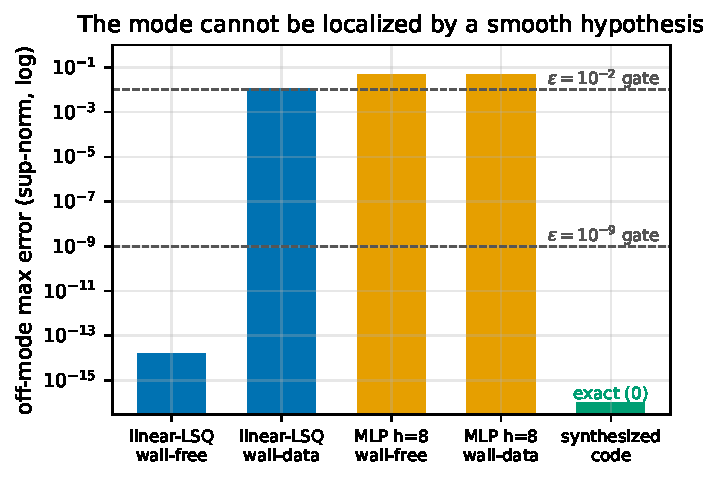
\includegraphics[width=0.6\textwidth]{figures/smooth_localization.pdf}
\caption{Off-mode max error (log) by model and training data. The wall-free linear fit sits at float noise and passes both gates (blind); four contact rows tilt it twelve orders of magnitude; synthesized code is exactly zero off-mode.}
\label{fig:smooth}
\end{figure}

\textbf{Identifiability is learner-independent, live.} On the wall-free sample the linear model recovers the off-mode dynamics to $10^{-15}$, \textbf{passes the $\varepsilon = 10^{-9}$ gate}, and is exactly as wall-blind as the synthesized blind code (probe error 4.18: it predicts straight through the wall). Proposition~\ref{prop:ident} instantiated on a second hypothesis class. The proposition's exact content is that on the miss event no sample-measurable score separates a mode-blind model from the true one, so acceptance carries no information about the mode --- not that every accepted model is blind, which is false and which this paper's own data refute: Claude's pendulum artifact was accepted while carrying an \emph{invented} mode, its prior having supplied off-sample content that happens to be wrong in the other direction. Blindness is what a prior-free learner gets; the identifiability event is what makes any of it possible. The $(1-r)^N$ hole is not an LLM property.

\textbf{With the mode in the data, code and smooth part ways.} Four contact rows out of 3200 tilt the linear fit by \textbf{twelve orders of magnitude} off-mode ($1.7\mathrm{e}{-14} \to 1.2\mathrm{e}{-02}$ max; Figure~\ref{fig:smooth}) --- it fails both gates \emph{and still} has the mode wrong (probe 4.17). The smooth hypothesis cannot put the error on the mode; it leaks everywhere (Proposition~\ref{prop:lipschitz}'s geometry, observed as a least-squares tradeoff). The synthesized code, on the \emph{same sample}, wrote the exact clamp and passed at float precision. The MLP combines both axes: a pervasive ${\sim}5\mathrm{e}{-3}$ floor that no gate accepts, and a never-learned mode.

Consequence for the CWM paradigm: the paradigm \emph{creates} in continuous control the localized failure class that the learned-model literature says does not dominate there --- and, by the same representational fact, also creates the exact-repair capability that learned models lack. Code cuts both ways, and the gate's sampling coverage decides which way.

\section{Related work}
\label{sec:related}

\emph{Objective mismatch and model exploitation in model-based RL} \citep{lambert2020objective,janner2019mbpo,hafner2020dreamer}: prediction accuracy and control performance diverge for learned continuous models; planners exploit model errors. Our contribution to that conversation is the \emph{verified-but-wrong localized} regime, which smooth learned models cannot even represent (Proposition~\ref{prop:lipschitz}, Table~\ref{tab:smooth}), plus a closed-form acceptance-failure law confirmed at gate scale. \emph{Hybrid systems:} mode detection and identification of piecewise/hybrid dynamics is classical \citep{paoletti2007hybrid,bemporad1999control}; our question is not identifying the mode but what a \emph{sampling verifier certifies} when the mode is missed, and what a planner then does. \emph{Code World Models} \citep{lehrach2025cwm} and code-as-policy \citep{liang2023codeaspolicies,gao2023pal} supply the paradigm; the companion paper \citep{aguilar2026verified} is the discrete study this paper extends --- transferring its provable core, showing its empirical residual (translation-not-inference) does not transfer, and adding the representational theorem separating code from smooth hypotheses. \emph{Property-based testing and rare events} \citep{claessen2000quickcheck,rubinstein2017montecarlo}: the gate is random testing of a program against an oracle; $(1-r)^N$ is the standard rare-input coverage gap, here with the planner as the adversary that finds it. \emph{Falsification and rare-event testing of hybrid and cyber-physical systems} \citep{annpureddy2011staliro,corso2021survey}: this literature searches for inputs that drive a hybrid system to violate a specification; our gate is the passive dual --- uniform random testing whose blind spot is precisely the rare mode a falsifier would hunt for, and the $(1-r)^N$ factor quantifies the coverage gap that random testing leaves. \emph{Runtime monitoring and shielding for safe RL and control} \citep{alshiekh2018shielding}: a synthesized shield overrides unsafe actions using an a-priori specification; our distrust-region fence is instead deployment-time feedback, built from observed prediction failures rather than a given safety automaton, and it corrects a certified-but-wrong model rather than an unsafe policy. \emph{Robust MPC and planning under model uncertainty} \citep{rawlings2017mpc}: robust and tube-based MPC guarantees performance against \emph{bounded} model error; the failure here is orthogonal --- the error is unbounded but localized to an omitted mode and is certified away by the gate, so robustness margins tuned to the off-mode error do not see it. \emph{System identification of contact-rich and discontinuous dynamics} \citep{paoletti2007hybrid,fazeli2017contact}: estimating parameters and contact forces of rigid bodies undergoing frictional contact is a mature sysid problem; our repair-from-data result is the code analogue --- given contact transitions in the sample, the synthesizer recovers the exact switching rule, whereas a smooth fit cannot localize it.

\section{Limitations and Honest Assessment}
\label{sec:limitations}

\paragraph{Three instruments; repair is geometry-scoped, mitigation fails outright on a 2D boundary at distance.} Cart-with-wall, pendulum-with-stop, and PatchField2D now span 1D and 4D state and one and two modes, so the earlier ``one dimension, single stationary boundary'' limitation no longer holds. The \emph{mechanism} survived every extension --- it is measure-theoretic --- and so did strict gate soundness (the all-or-nothing 2D gate certified no partial artifact). The honest residue is now sharper and different. \textbf{Repair-from-data collapses on 2D region boundaries, curved or flat}: GPT-5.x repaired 109 of 111 revealed 1D clamps but recovered the 2D region rule in 0/156 mode-containing attempts over 20 distinct gate samples pooled over the disc, the square ablation, and the guided/$3\times$-budget treatment (Section~\ref{sec:patch2d-synthesis}). The prompting/budget and curvature outs are now \emph{measured negatives}; what could restore repair --- two-sided (inside) evidence, active boundary probing, or richer evidence summaries --- is the subject of ongoing follow-up work. The \textbf{2D mitigation} likewise generalizes but only partially, and its failure mode at the farthest knob is not a longer transient but lock-in: $7$ of $20$ episodes end pinned at blind-level return, because the fence's tie-break is an unsigned distance and a curved boundary lets the planner be pinned against it (Section~\ref{sec:patch2d-mitigation}). A signed outward normal is the obvious fix and is untested. Contact-rich manipulation, moving boundaries, and $3{+}$ modes remain future work.

\paragraph{Two planner families, one fixed configuration each.} Random-shooting MPC sits at the high-query-reach/high-play-cost end and CEM at the low-query-reach/near-zero-play-cost end (Section~\ref{sec:cem}); only the latter is \emph{implied} by Proposition~\ref{prop:playcost}, since the bound forces low play cost from low reach but does not force the converse. This is stronger than a one-family result but not planner-universal: CEM was measured at one prototype-fixed setting, with no hyperparameter sweep, and its pendulum truth returns expose local optima. Its non-exploitation is reach-limited, not knowledgeable or safe --- the same search that misses phantom reward can miss real distant reward. Gradient-based shooting and tree search \citep{coulom2006mcts,kocsis2006bandit} remain untested. Distrust-region replanning (Section~\ref{sec:mitigation}) is a mitigation layered on MPC, not a third family; its hard-boundary guarantee and its behavior with other planners remain untested.

\paragraph{Synthesis cells are modest, and the two sizes share their samples.} The gate sample is drawn from the seed index alone, so mini and large are synthesized from identical samples at every instrument and knob (Section~\ref{sec:synthesis}): every pooled ``both sizes'' count is $n$ distinct gate samples with two synthesis draws each, and the distinct-sample $n$ is half the pooled one --- 10 mode-absent samples on the cart headline cell, 31 mode-present across the two pendulum knobs, 38 mode-containing on the PatchField2D disc cells, 20 on each ablation campaign. Per-size Wilson bounds are quoted for exactly this reason wherever only shared blocks exist. On the two \emph{headline} cells the constraint was removed instead: the large arm was re-run on a disjoint seed block (\texttt{-{}-seed-offset 20}), so there the pooled counts are over independent samples, the Wilson bounds are legitimate ($0.84$ cart, $0.796$ pendulum), and even the $(1-r)^N$ gate-miss check becomes poolable ($20/40$ independent cart samples lacked the mode against a predicted $0.63$). With that accounting: 20 seeds/cell on the headline $x_\mathrm{wall} = 8$ cart cell for both GPT-5.x sizes, plus a 3-seed Qwen cross-family spot-check; the pendulum arm adds two knobs (headline and caught) at the same 20 seeds/cell, both sizes, plus its own 3-seed Qwen spot-check. The wall/mode-absent conditional is 20/20 across cart sizes and three runs and 18/18 across pendulum sizes: per size that is 10/10 (Wilson lower bound 0.72) and 9/9 (0.70), the bounds we rely on, against pooled 0.84 and 0.824 whose trials share samples. The GPT-5.x repair rate is 20/20 on the cart headline cell and 62/62 pooled on the pendulum (31 distinct samples). The cross-family arms are small-$n$ (3 seeds plus one control per instrument per family) and cover two alternate families (Qwen, and Claude agent-relayed), not a sweep of models --- and their coverage is uneven across instruments: both families were run on the two 1D instruments, but on PatchField2D only Claude has an incomplete arm --- the Qwen run there aborted after its three full-arm cells when that provider's inference credits were exhausted, so it is a translation control (3/3 exact) with no induction data, a gap of circumstance rather than of judgement; they show repair is model-dependent \emph{in mechanism} --- Qwen 0/2 mode-present (superstitious patches), Claude repairing most but via a symmetry prior that oscillated on two seeds and certified one phantom, unfalsifiable mode. The PatchField2D synthesis arm adds two bi-knob cells (20 seeds each, both GPT-5.x sizes) plus two ablation campaigns (region-guidance $3\times$ budget; zero-curvature square --- 20 seeds each, both sizes); its finding is a \emph{negative} one --- 0/76 repair of the circular mode, 0/66 partial repair, 0/156 pooled, plus 0/3 in a Claude cross-family arm on the same cell whose failure classes match (Section~\ref{sec:patch2d-synthesis}) --- so repair-from-data is not only model-dependent but geometry-dependent, via a template prior.

\paragraph{The mode-blindness probe covers only the true mode's region.} By construction \texttt{mode\_blindness} (\texttt{src/cwm/continuous/contract.py}) fires probes where the truth's mode is active, so it certifies whether the \emph{revealed} mode is encoded but is blind to a mode the model \emph{invents} elsewhere: Claude's phantom pendulum stop (Section~\ref{sec:synthesis}) scored blindness 0.0 while carrying an extra, non-existent stop at $\theta = -1.4$. Detecting invented modes needs code inspection, or probes seeded outside the sampled region --- the classification alone does not suffice, and our phantom-mode finding rests on reading the certified code, as the companion paper's artifact-level analysis does.

\paragraph{The MLP is a probe, not a baseline.} It substantiates the representational point at $h{=}8$/pure-Python scale; a tuned modern dynamics model would have a lower floor but the same structural inability to be bit-exact off a mode at $\varepsilon = 10^{-9}$ (an argument, not yet a measurement, at scale).

\paragraph{Proposition~\ref{prop:lipschitz} bounds geometry, not probability.} The ball is metric; converting to gate-visitation probability needs the gate measure on that ball, which is instrument-specific. The empirical complement (Table~\ref{tab:smooth}'s twelve-orders tilt) carries the quantitative weight here.

\paragraph{Coverage certificates transfer, but only to the smooth case.} The companion paper's guarantees enumerate information sets, and that enumeration has no continuous analogue. What does transfer is the covering-number version: Proposition~\ref{prop:coverage} certifies $\sup_U \|f - \hat f\| \leq \varepsilon + 2L\rho$ for $L$-Lipschitz pairs once the gate $\rho$-covers $U$, with the sample size a covering number over a visitation density, and on the deployed cart gate it excludes a pair with $L = \max(\mathrm{Lip} f, \mathrm{Lip}\hat f) \leq 5.77$ carrying the wall's error magnitude of $4.2$, with probability at least $1-\delta$ over gate draws, against a rigorous bound of $0.933$ on the step-1 reachable set. Since the bound $\varepsilon + 2L\rho$ grows with $L$, that quantifier is the claim's scope, and at $4.5\times$ the plant's own $1.27$ it is a broad class. Getting there took replacing a packing argument with a \emph{partition} argument: three of the errors this section had to correct were geometric factors that a packing bound has to estimate (the covering-vs-packing direction, the ball's intersection with $U$, and the corner factor's failure to be shear-invariant), and a partition bound estimates none of them --- on this instrument the step-1 law is uniform on a sheared box, so equal sub-boxes have probability exactly $1/K$. The packing route's own honest figure was $\rho = 1.165$ and $2.97$, licensing only $L \leq 1.80$. The honest residue is that this is exactly the case the paper is \emph{not} about: the hybrid mode has unbounded local Lipschitz constant, so no finite $L$ makes the certificate apply to it, and the danger the paper measures lives entirely in that gap. Two gaps that we had listed as open are now closed, and closing them made the certificate \emph{weaker} and the conclusion sharper. Closed: the within-rollout dependence, which needs no mixing argument and, as it turns out, no factorization either --- the per-rollout miss probability is measured directly and the i.i.d.-ness of rollouts raises it to the $N$th power exactly. Composed with the partition, that is what gives the $0.933$ above, against $1.534$ from independent single samples: handling the dependence honestly is worth a factor of $1.6$, and the all-steps-independent reading's $0.785$ was optimistic by only $1.2$ rather than unreachable. On a box $6.7\times$ larger the same treatment certifies net radius $1.0$, which is the region/resolution trade-off at fixed $N$ rather than a competing figure. Also closed: the density is derived at \emph{every} step $t \geq 2$ (the last two actions make the step-$t$ law absolutely continuous with an exact constant $1/0.036$, and a Minkowski erosion turns that into a pointwise infimum). That extends the certificate to larger regions, but at fixed $N$ extent is paid for with resolution, and no step-$t$ level set certifies a bound below the step-1 figure --- so what limited the certificate was never the step-1 restriction but the gate's size. The nonlinear analogue is not a separate case: the two-action Jacobian determinant is $\mathrm{gain}^2 dt^3$ identically for any $C^1$ force, so the same constant serves the cart and the pendulum, and it degenerates only on the mode clamp, where no density argument can work because the truth maps a neighborhood to a point. And the planner-versus-gate mismatch is measured rather than argued: the box the dependence-exact certificate covers carries $1.9\%$ of the exploited planner's queries, and a box containing every step-$t$ level set carries $7.8\%$ --- an upper bound on the certified share. What is left is therefore not a hole in the argument but its conclusion --- a sound certificate on a region the planner barely visits. Certifying the planner's own visitation would need a gate that samples it, which is precisely the change the companion paper's closing prescription asks for.

\paragraph{play\_cost $> 1$ is a normalization artifact} (blind $<$ random), reported unclamped and explained; the headline claims never depend on the excess over 1.

\section{Conclusion}
\label{sec:conclusion}

The companion paper ended by diagnosing the gate failure as a reach-distribution shift and prescribing verification on the distribution the planner visits. This paper shows the diagnosis is not about discreteness. The gate-miss law, the identifiability argument, and the play-cost bound are measure-theoretic and survive the move to continuous state spaces intact; what the move changes is \emph{where the localized failure can live} (hybrid mode boundaries --- an omitted mode is a rare rule) and \emph{who can express it} (programs, not smooth function classes: Proposition~\ref{prop:lipschitz} and Table~\ref{tab:smooth}). On two minimal hybrid instruments the entire discrete phenomenology reproduces --- threshold law, knob-invariant exploitation, the reach mechanism --- with the gate's acceptance rate closely tracking $(1-r)^N$ at gate scale (within sampling noise; Section~\ref{sec:axes}).

The synthesis experiment then delivers this paper's own finding: on the 1D instruments the continuous regime is the one where the danger law is \emph{everything}. Given the mode in its sample, the LLM repairs it exactly --- including from the synthesis examples alone --- and when it fails to repair, the gate catches the superstitious patch; given the mode absent, every learner we tried (LLM, exact linear regression) is certified blind and the planner is exploited to below-random performance. That repair, though, is geometry-dependent: on a third, 4D bi-modal instrument with 2D modes it inverts --- neither GPT-5.x size recovers the region rule from data (0/156, including a zero-curvature square and a guided $3\times$-budget treatment: a template prior over region forms, not curvature), and a second family fails in the same classes, and the danger law's exhaustiveness is scoped back to the 1D clamps, though the gate stays sound (Section~\ref{sec:patch2d-synthesis}). The provable core is the gate-miss and identifiability propositions (Section~\ref{sec:theory}): the mode-absent event is a hole no learner can close \emph{from the sample} --- a prior or the specification could still supply the mode --- and its probability is in closed form. Sample-covered exactness is the acceptance criterion itself; that accepted artifacts were also right off-sample --- with the single phantom-mode exception, wrong only where its sample is silent --- is an empirical regularity of the models tested (GPT-5.x repairs; Qwen stalls and is refused; Claude repairs most through a symmetry prior), not a theorem. For practitioners the message is one clause sharper than the discrete one: in continuous code-world-model pipelines, \emph{sample coverage of the mode boundaries is the whole game} --- the synthesis stack will translate what it is told and repair what it is shown, and no stage of it can \emph{learn from the sample} what the sample never touched (a prior or the specification still can, and Claude's did).

\appendix

\section{Reproducibility}

All code is at \url{https://github.com/JaviMaligno/code-world-models} (\texttt{src/cwm/continuous/}, \texttt{scripts/continuous\_*.py}); the experiment log is \texttt{docs/EXPERIMENTS.md} (sections prefixed ``PAPER 2'') and per-seed artifacts, including every synthesized program, are versioned under \texttt{results/}. CPU results (Tables~\ref{tab:danger}--\ref{tab:smooth}):

\begin{verbatim}
PYTHONPATH=src python scripts/continuous_reach.py
                     # danger-curve table (tab:danger; ~2.5 min)
PYTHONPATH=src python scripts/continuous_axes.py
                     # axis-separation table (tab:axes; ~3 min)
PYTHONPATH=src python scripts/continuous_smooth_probe.py
                     # smooth-learner table (tab:smooth; ~11 s)
PYTHONPATH=src python scripts/continuous_pendulum.py
                     # pendulum table (tab:pendulum; ~2 min)
PYTHONPATH=src python scripts/continuous_cem.py
                     # second planner family (tab:cem; ~29 min)
PYTHONPATH=src python scripts/continuous_patch2d.py
                     # PatchField2D mechanism (tab:patch2d)
PYTHONPATH=src python scripts/continuous_cem_patch2d.py
                     # PatchField2D CEM rows (sec:cem; ~14 min)
PYTHONPATH=src python scripts/continuous_eps_sweep_patch2d.py
                     # PatchField2D eps rows (tab:eps-sweep text; ~8 min)
PYTHONPATH=src python scripts/continuous_mitigation_patch2d.py
                     # PatchField2D mitigation (tab:patch2d-mitigation)
PYTHONPATH=src python scripts/phantom_targeting_probability.py
                     # what the plan provably chases (sec:mechanism; ~4 min)
PYTHONPATH=src python scripts/play_cost_proved_bounds.py
                     # derived J_max / J_min + oracle (prop:normalizers; ~3 min)
PYTHONPATH=src python scripts/eps_flatness_rate.py
                     # the quadratic flatness rate (prop:epsrate; ~6 min)
PYTHONPATH=src python scripts/gate_partition_certificate.py
                     # the partition certificate: exact (a) + all-steps (b)
                     # (prop:partition; ~25 min)
PYTHONPATH=src python scripts/gate_partition_validation.py
                     # 400 gates against the certificate's own partition (~4 min)
PYTHONPATH=src python scripts/patch2d_dependence_50k.py
                     # dependence sign at 50k rollouts (rem:bracket; ~40 min,
                     # resumable per knob)
PYTHONPATH=src python scripts/fence_separation_census.py
                     # fence placement, eps-invariance, 2D per-episode census
                     # (sec:mitigation; ~12 min)
PYTHONPATH=src python scripts/sample_stream_census.py
                     # distinct rollout-seed blocks per campaign (instant)
python scripts/make_paper2_figures.py     # figures from the JSONs
python scripts/audit_paper2_numbers.py    # re-derive every table cell
                     # (and the counted prose claims) from the JSONs
\end{verbatim}

LLM arms (Azure credentials in \texttt{.env}; the runbook --- commands, cost,
predictions, troubleshooting --- is the section ``Runbook --- LLM arms'' of the
design spec under \texttt{docs/specs/}, dated 2026-07-06):

\begin{verbatim}
PYTHONPATH=src python scripts/continuous_danger_synthesis.py mini 5
PYTHONPATH=src python scripts/continuous_danger_synthesis.py mini 5 --x-wall 4
PYTHONPATH=src python scripts/continuous_danger_synthesis.py large 5
# Pendulum synthesis arm (second instrument; Azure credentials as above)
PYTHONPATH=src python scripts/continuous_danger_synthesis.py mini 20 \
  --instrument pendulum --th-stop 1.4
PYTHONPATH=src python scripts/continuous_danger_synthesis.py large 20 \
  --instrument pendulum --th-stop 1.4
PYTHONPATH=src python scripts/continuous_danger_synthesis.py mini 20 \
  --instrument pendulum --th-stop 1.0
PYTHONPATH=src python scripts/continuous_danger_synthesis.py large 20 \
  --instrument pendulum --th-stop 1.0
# Qwen cross-family spot-checks
# (needs HF_TOKEN: HF Inference Providers router)
PYTHONPATH=src python scripts/continuous_danger_synthesis.py mini 3 \
  --compat-model "Qwen/Qwen3-Coder-30B-A3B-Instruct"
PYTHONPATH=src python scripts/continuous_danger_synthesis.py mini 3 \
  --instrument pendulum --th-stop 1.4 \
  --compat-model "Qwen/Qwen3-Coder-30B-A3B-Instruct"
# Claude agent-relayed cross-family spot-checks (agent scaffold relays
# pipeline-identical messages; see scripts/continuous_claude_step.py,
# results/continuous_claude_relay.json + results/claude_relay_transcripts/).
# One relay round = init (writes msgN.txt) -> relay it -> check (gates the
# reply, writes msgN+1.txt or classifies). The 2D arm, per seed:
PYTHONPATH=src python scripts/continuous_claude_step.py init 10000 \
  results/claude_relay_transcripts --instrument patch2d --k1 3 --k2 7 \
  --arm incomplete
PYTHONPATH=src python scripts/continuous_claude_step.py check 10000 \
  results/claude_relay_transcripts 0 REPLYFILE --instrument patch2d \
  --k1 3 --k2 7 --arm incomplete --model-label "claude-sonnet-5 (agent-relayed)"
# Per-iteration ledger, re-derived from the versioned transcripts (CPU only):
PYTHONPATH=src python scripts/claude_relay_ledger.py \
  results/claude_relay_transcripts --tag patch2d_k3_7 --k1 3 --k2 7
# PatchField2D synthesis arm (4D bi-modal; two bi-knob cells)
PYTHONPATH=src python scripts/continuous_danger_synthesis.py mini 20 \
  --instrument patch2d --k1 3 --k2 7
PYTHONPATH=src python scripts/continuous_danger_synthesis.py large 20 \
  --instrument patch2d --k1 3 --k2 7
PYTHONPATH=src python scripts/continuous_danger_synthesis.py mini 20 \
  --instrument patch2d --k1 5 --k2 9
PYTHONPATH=src python scripts/continuous_danger_synthesis.py large 20 \
  --instrument patch2d --k1 5 --k2 9
# Mitigation sweep (CPU only)
PYTHONPATH=src python scripts/continuous_mitigation.py
# eps-sensitivity sweep (CPU only)
PYTHONPATH=src python scripts/continuous_eps_sweep.py
\end{verbatim}

\bibliography{references}

\end{document}
